\documentclass[12pt]{report}
\usepackage[utf8]{inputenc}
\usepackage[spanish]{babel}
\usepackage{color, soul}
\usepackage{graphicx}
\usepackage{amsmath}
\usepackage{verbatim} %para comentarios multilinea
\graphicspath{{figuras/}}
\usepackage[left=3cm,right=3cm,bottom=3.5cm,top=3.5cm]{geometry}
\usepackage{cite}
\usepackage{gensymb} %este paquete habilita el uso del simbolito de grados centígrados \degree
\usepackage{rotating} %este paquete permite rotar una tabla para que quede vertical y en toda la página
\usepackage{caption} %$este paquete se necesita para el subcaption
\usepackage{subcaption} %$este paquete permite tener subfiguras
\usepackage{amsfonts} % para usar R como conjunto de números reales

\newcommand{\paginaenblanco}{\clearpage\mbox{}\newpage}

\title{
	{\large Análisis y detección de correlaciones en relevamientos transcripcionales de gran escala}\\
    {Tesis de Licenciatura en Ciencias Físicas}\\
	{\large Facultad de Ciencias Exactas y Naturales}\\
	{\large Universidad de Buenos Aires}
}
\author{Andrés Rabinovich}
\date{Marzo 2016}

\begin{document}

%--------------------DESDE ACA LOS COMENTARIOS-------------------
\maketitle
\paginaenblanco
\chapter*{Hoja a completar por los jurados}
\paginaenblanco
\chapter*{Resumen}
\paginaenblanco
\chapter*{Abstract}
\paginaenblanco
\chapter*{Dedicatoria}
\paginaenblanco

\tableofcontents

\chapter*{Motivaciones y objetivos}
La genómica funcional es un campo de la biología molecular que hace extenso uso de datos genómicos y transcriptómicos para estudiar, describir y responder preguntas acerca de la expresión, función e interacción de genes y proteínas en una escala global (a lo largo de todo el genoma), en contraposición con los métodos más tradicionales de estudio que se realizan gen por gen.\\
Desde principios del año 2000, a partir de la aparición de tecnologías experimentales modernas, tales como la tecnología de Micromatrices de ADN (DNA microarray), secuenciadores de nueva generación (NGS) o secuenciadores de ARN (RNAseq), es posible relevar el estado transcripcional de una célula de forma global, es decir, cuantificar los niveles de todo el RNA mensajero que está siendo exportado en un dado momento desde el núcleo celular hacia el citoplasma con el fin de producir determinadas proteínas.\\
La realización de este tipo de estudios posee un potencial enorme, con aplicaciones tanto en áreas de investigación básica como aplicada, investigaciones biomédicas, farmacológicas y de la salud.\\
En particular, en relevamientos transcripcionales de gran escala es posible obtener información sobre el nivel de activación de miles de genes, para decenas o cientos de condiciones ambientales/experimentales diferentes. Para ganar conocimiento biológico a partir de la cantidad enorme de datos que estos relevamientos generan, es necesario implementar estrategias de búsqueda de correlaciones en espacios de alta dimensionalidad.\\
Para ello, es de fundamental importancia el estudio e implementación de procedimientos de búsqueda de estructuras aplicables a este tipo de relevamientos, cobrando predominancia técnicas estadísticas y técnicas de aprendizaje automático no supervisado, tales como las técnicas de agrupamiento o ``clustering'', que permitan reconocer subconjuntos de genes que evidencien patrones de coexpresión similares a lo largo de conjuntos específicos de condiciones experimentales.\cite{functional_genomics_definition_nature, functional_genomics_definition_wikipedia}

\section*{Objetivos y organización de la tesis}
El presente trabajo tiene como objetivo analizar la coherencia entre la métrica transcripcional y la inferida a partir de otros espacios de conocimiento, como ser redes de interacción de proteinas (PIN por sus siglas en ingles), redes inferidas de literatura curada (LCI), vías metabólicas (KEGG) y ontología genética (GO).

\hl{Vamos a haerlo cuantitativamente y tartar de incorporar lo encontrado en la elaboracion de metricas mixtas que permitan clusterear perfiles y obtener estructuras compactas (coherentes) en varios espacios. Para esto Vamos a usar dataset de wiegel (presentarlo someramente) y PIN y LCI del paper tal y GO de tal lugar}\\
\hl{Curado manual y de ontologia para ver que hay informacion biologica contenida en clustering por coexpresion}\\\\
Está tesis está organizada de la siguiente forma. En el capítulo 1 se introdujeron los conceptos biológicos necesarios para comprender y motivar los datos presentados y analizados. En el capítulo 2 introduciremos los materiales y métodos utilizados a lo largo del trabajo. Describiremos la composición y funcionamiento de los métodos de obtención de los cuatro tipos de datos que analizaremos (micromatrices de ADN, redes de interacción de proteínas, redes de vías metabólicas y ontología GO). En el capítulo 3 presentaremos en detalle los métodos de agrupamiento de datos utilizados en este trabajo y analizaremos las problemáticas asociadas a cada uno. En el capítulo 4 analizaremos los datos mediante los métodos presentados en el capítulo 3 y los caracterizaremos buscando información biológica en los mismos. En el capítulo 5 utilizaremos la información obtenida en el capítulo 4 para proponer una métrica mixta que permita aumentar la cantidad de información biológica obtenida previamente. Finalmente, en el último capítulo analizaremos los resultados obtenidos y plantearemos futuras lineas de estudio.
\chapter{Introducción biológica}
Este capítulo tiene por objetivo el introducir al lector en los conceptos biológicos básicos necesarios para comprender y motivar los datos presentados y analizados en este trabajo. El lector que desee profundizar sobre los mismos puede remitirse a \cite{Domany2003, Alberts2015}.
\section{Información hereditaria: ADN}
Las células y los organismos pueden ser divididos en dos ramas, procariotas (como las bacterias) y eucariotas (como las plantas, hongos y animales). En las procariotas, el material genético no ocupa una región definida dentro de la célula, sino que se encuentra disperso en el citoplasma, mientras que en las eucariotas, el material genético se encuentra separado del citoplasma en una región denominada núcleo (figura \ref{fig:celula_eucariota}).\\\\
Todas la células vivas de La Tierra transmiten su información genética hereditaria por medio del ADN (ácido desoxirribonucleico). El ADN es una molécula unidimensional formada por dos hebras enrolladas una alrededor de la otra en una estructura de doble hélice (figura \ref{fig:adn1}). Las hebras son cadenas largas de polímeros formadas por monómeros (los nucleótidos), que consisten en dos partes: una columna conformada por un azúcar (desoxirribosa) con un grupo fosfato adherido, y una base nitrogenada, que puede ser adenina (A), guanina (G), citosina (C) o tiamina (T). Cada azúcar se conecta al siguiente mediante un grupo fosfato, con una protuberancia formada por la base, creando de esta manera una cadena polimérica. 
\begin{figure}[h]
    \centering
    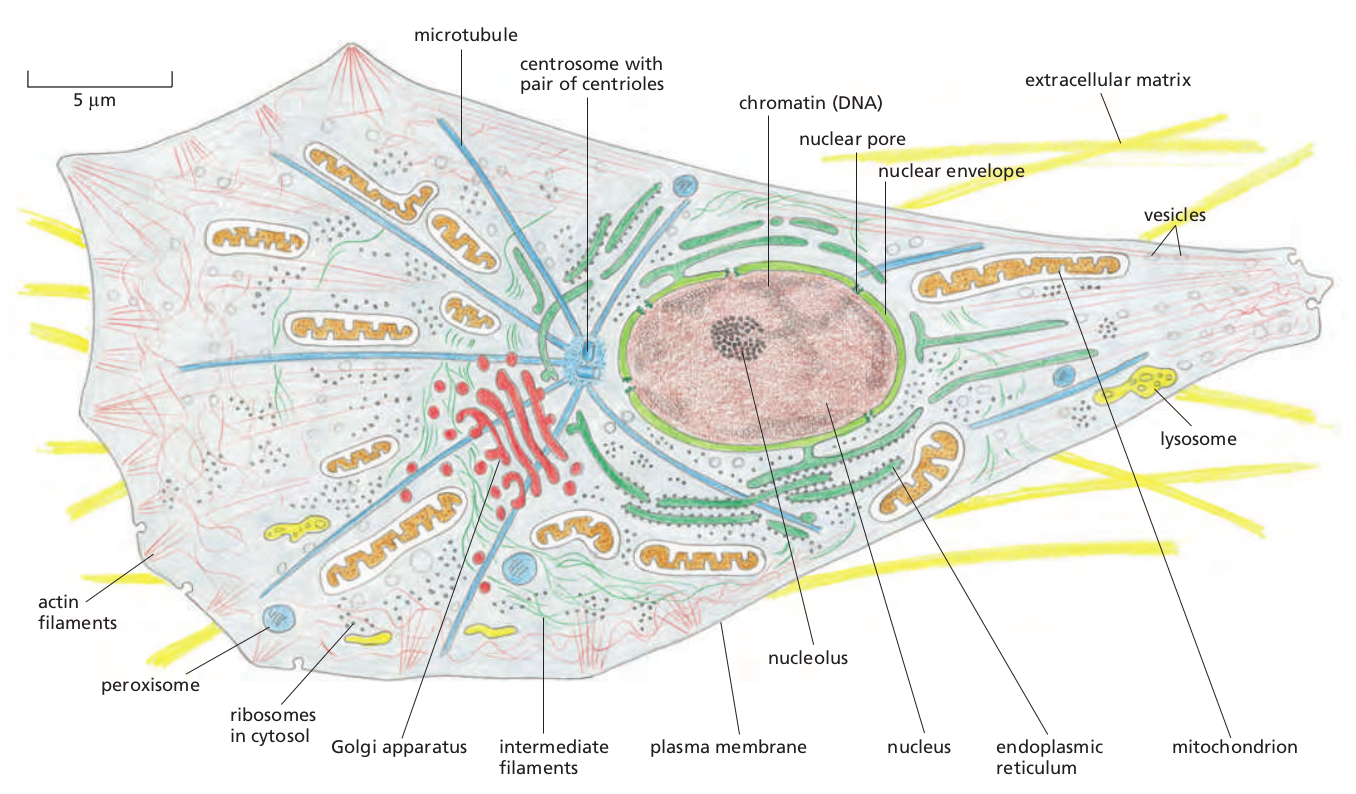
\includegraphics[width=0.8\textwidth]{celula_eucariota}
    \caption{La célula eucariota y sus principales características, entre las que se destacan los ribosomas y el núcleo conteniendo al ADN. (Fuente: Alberts \cite{Alberts2015})}
    \label{fig:celula_eucariota}
\end{figure}
En principio, es posible extender la cadena de ADN agregando cualquier monómero al final de la misma. Sin embargo, el ADN no se sintetiza como una única hebra, sino a partir de una hebra preexistente, por lo que cada nucléotido debe conectarse mediante puentes de hidrógeno con un nucléotido de la hebra preexistente siguiendo unas reglas estrictas definidas por la estructura complementaria de las bases: A se conecta con T (mediante dos puentes de hidrógeno) y C con G (mediante tres). De esta manera, se forma la estructura de doble hélice con hebras complementarias del ADN. Las uniones entre las bases son mucho más débiles que entre los azucares y los grupos fosfato, lo que permite a las hebras separarse sin que se rompan.\\\\
\begin{figure}[h]
    \centering
    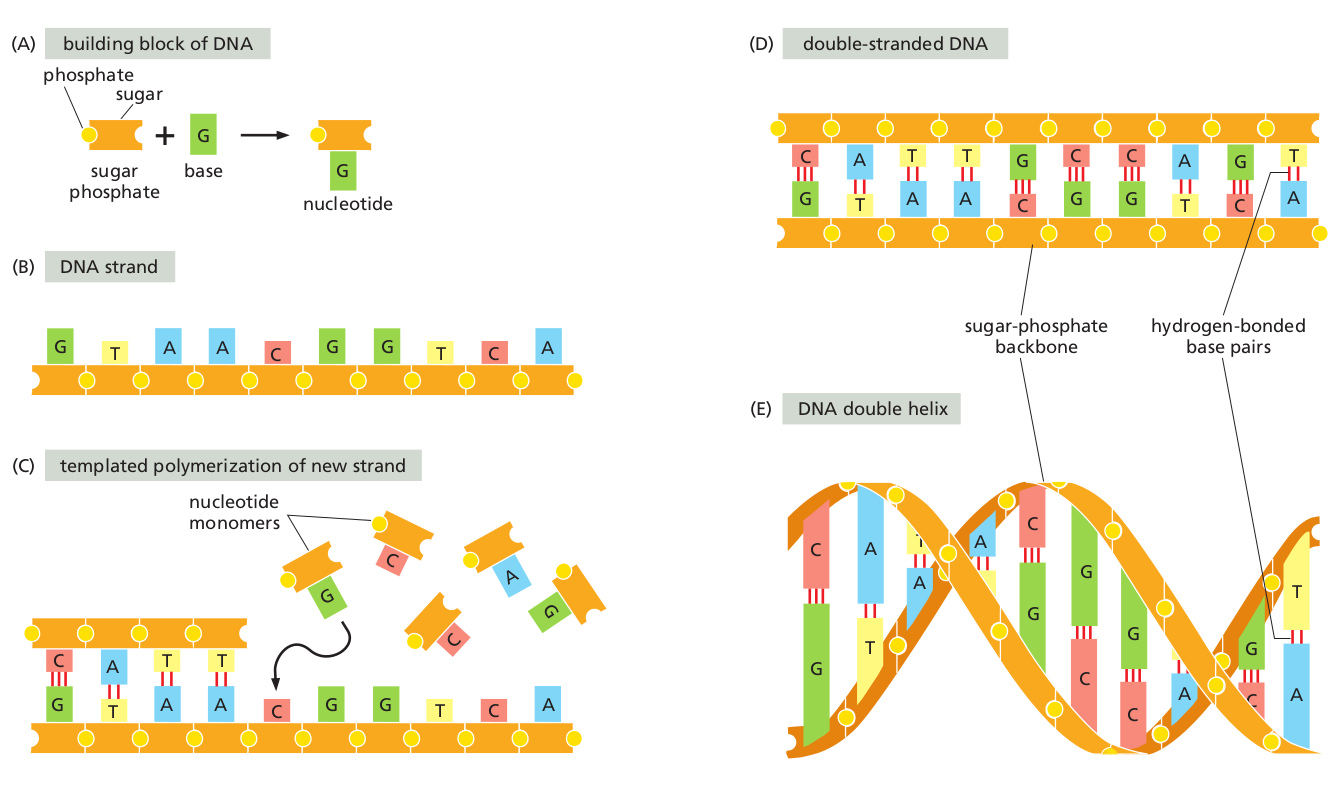
\includegraphics[width=0.8\textwidth]{adn1}
    \caption{Información hereditaria en el ADN. (A) Bloques constitutivos del ADN, esqueleto azúcar-fosfato y base nitrogenada. (B) Una hebra de ADN compuesta por el esqueleto de azucares-fosfatos y las bases. (C) Polimerización de una hebra a partir de otra que funciona como plantilla. (D) ADN completo con las dos hebras. (E) Forma final del ADN con las hebras en configuración de dóble hélice. (Fuente: Alberts \cite{Alberts2015})}
    \label{fig:adn1}
\end{figure}
Un gen es un segmento de ADN que contienen la información necesaria para la síntesis de una proteína en particular. Las proteínas son las moléculas que llevan a cabo casi todos los procesos dentro de una célula, y están compuestas por hasta 20 aminoácidos diferentes. Un gen es por lo tanto una receta que indica el orden en que se colocarán estos aminoácidos, codificada en la secuencia lineal de bases en la molécula de ADN. El genoma es la colección de todos los genes que codifican todas las proteínas que un organismo requiere para vivir. El genoma de un organismo sencillo como el de la levadura contiene alrededor de 6000 genes, mientras que el del humano contiene entre 30000 y 40000. La mayor parte del ADN humano (un 98\%) contiene regiones no codificantes, es decir, hebras que no codifican ninguna proteína en particular. Aunque en un principio se pensaba que esta enorme proporción del genoma no cumplía funcionalidad alguna (se hablaba del genoma basura o ``garbage genome'' en inglés), estudios recientes sugieren que, al menos en algunos casos, podría jugar un rol regulatorio en la síntesis de ciertas proteínas.\\\\

\section{Transcripción y traducción: dogma central de la biología molecular}
Para poder llevar a cabo la función de transmitir información, el ADN debe poder hacer algo más que replicarse. Debe poder expresar esa información que permite la síntesis de otras polímeros: el ARN y las proteínas.\\\\
El proceso para la síntesis de una proteína se conoce como transcripción y comienza con la síntesis de una molécula más corta de un polímero llamado ARN (ácido ribonucléico). En el ARN, la columna está conformada por el azucar ribosa y cuatro bases, urancil (U) en lugar de tiamina, y las otras tres bases A, C y G son las mismas que en el ADN, apareándose cada una con su respectiva base complementaria. Durante la transcripción, las hebras de ADN se separan en la región a ser copiada y los monómeros que conforman el ARN son conectados con sus bases complementarias en el ADN (figura \ref{fig:adn2}).\\ 
\begin{figure}[h]
    \centering
    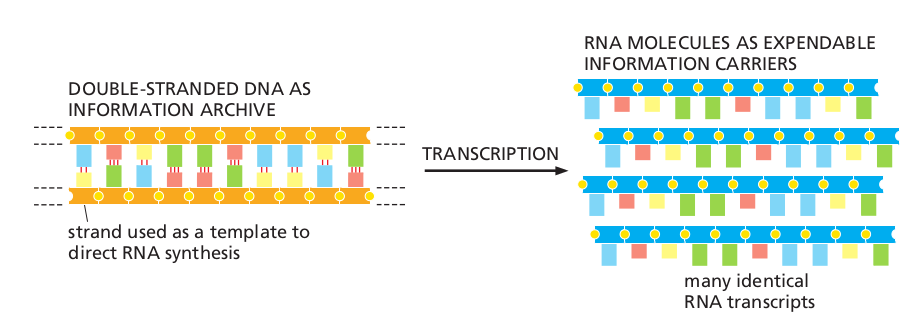
\includegraphics[width=0.8\textwidth]{adn2}
    \caption{Proceso de transcripción de información genética. Lo doble hebra del ADN se separa y cada hebra sirve como plantilla para la síntesis de ARN. (Fuente: Alberts \cite{Alberts2015})}
    \label{fig:adn2}
\end{figure}
La molécula de ARN final es una secuencia que reproduce fielmente la información del gen copiado, donde cada triplete de bases consecutivas (llamados codones) codifica cada aminoácido de la proteína a sintetizar, y es esta molécula la que es exportada desde el núcleo al citoplasma en forma de ARN mensajero (ARNm), dejando la información original intacta dentro del núcleo celular.\\\\
Esta molécula de ARNm será luego utilizada por el ribosoma, una maquinaria catalítica compleja consistente en más de 50 proteínas ribosomales diferentes y varias moléculas de ARN ribosomal, para sintetizar la proteína codificada por el gen, en un proceso llamado traducción. Todo el proceso completo de transcripción y traducción se conoce como dogma central de la biología molecular.
\begin{figure}[h]
    \centering
    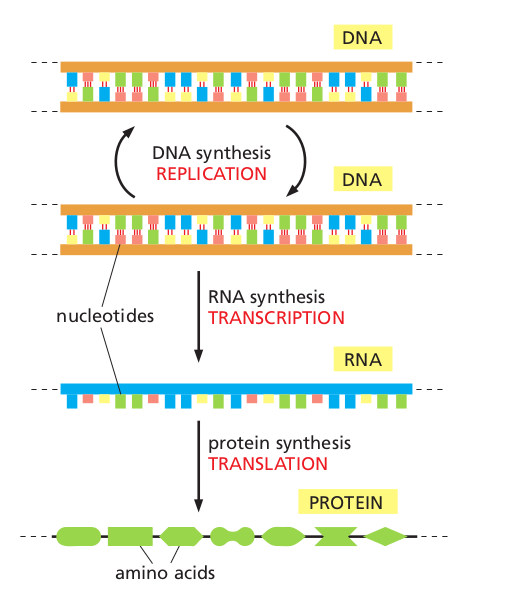
\includegraphics[width=0.5\textwidth]{adn3}
    \caption{Proceso de transcripción y traducción de información genética: dogma central de la biología molecular. El ADN se replica, se transcribe a ARN y luego se traduce a una proteína. (Fuente:Alberts \cite{Alberts2015})}
    \label{fig:adn3}
\end{figure}
Si bien cada célula que compone un organismo complejo posee el mismo ADN, células tomadas de distintos órganos realizan diferentes funciones, al igual que las proteínas en los mismos. Por ejemplo, las células de la retina requieren moléculas fotosensibles, mientras que las células que componen el hígado no las requieren. Existe entonces un proceso conocido como diferenciación dentro de cada célula. En lugar de sintetizar todas las posibles proteínas, la célula regula los niveles de transcripción y traducción de los genes que codifican las proteínas necesarias para la misma y únicamente esas proteínas son las que serán sintetizadas.\\\\
En un dado momento, la célula puede requerir muchas proteínas de un tipo y pocas de otro, es decir, en un dado momento cada gen individual puede expresarse a niveles diferentes. La transcripción de un gen (la orden de comenzar a copiarlo o de finalizar la copia) es regulada por proteínas especiales llamadas factores de transcripción, que se ligan a regiones específicas del ADN fuera de la región codificante, que inician o suprimen la transcripción. Esto lleva a la asunción en que se basa el análisis de expresión genética: el estado biológico de una célula queda determinado por su perfil de expresión, es decir, los niveles de expresión de cada gen individual en el genoma, que pueden ser inferidos a partir de las concentraciones de ARNm.\\\\
Conocer cuales son los genes que se expresan frente a determinados estímulos, puede brindar información sobre la función que realizan las proteínas codificadas por los mismos en el organismo, información clave para comprender las bases de enfermedades complejas como el cáncer.
\chapter{Materiales y Metodos}
Las técnicas de relevamientos transcripcionales de gran escala, tales como las micromatrices de ADN y secuenciamientos de ARN (secuenciadores de próxima generación), permiten el monitoreo en paralelo de la totalidad del genoma. En este capítulo daremos una introducción al funcionamiento del primer tipo de tecnologías, que será la que usaremos extensivamente en este trabajo, y a los diferentes conjuntos de datos que utilizaremos.\cite{Bose2016}

\section{Micromatrices de ADN}
La tecnología de micromatrices de ADN se constituyó como una herramienta indispensable para el monitoréo de niveles de expresión a lo largo de todo el genoma de un organismo, estimando la concentración de ARNm que está siendo exportado desde el núcleo celular hacia el citoplasma para la síntesis de determinadas proteínas.\\
Una micromatriz es típicamente un portaobjetos de vidrio u otra superficie sólida a la cual se le adosan de forma ordenada y en lugares específicos (llamados sondas) moléculas de ADN. Un mismo sitio puede contener varios millones de copias de moléculas idénticas de ADN de composición conocida (tanto genómico como hebras cortas de oligo-nucleótidos) que se corresponden de forma unívoca con un gen. Una micromatriz de ADN puede medir en simultaneo los niveles de expresión de hasta 40000 genes distintos.\\
Dependiendo de la tecnología utilizada, las micromatrices pueden ser de canal único o de doble canal.\\
\begin{figure}[h]
    \centering
    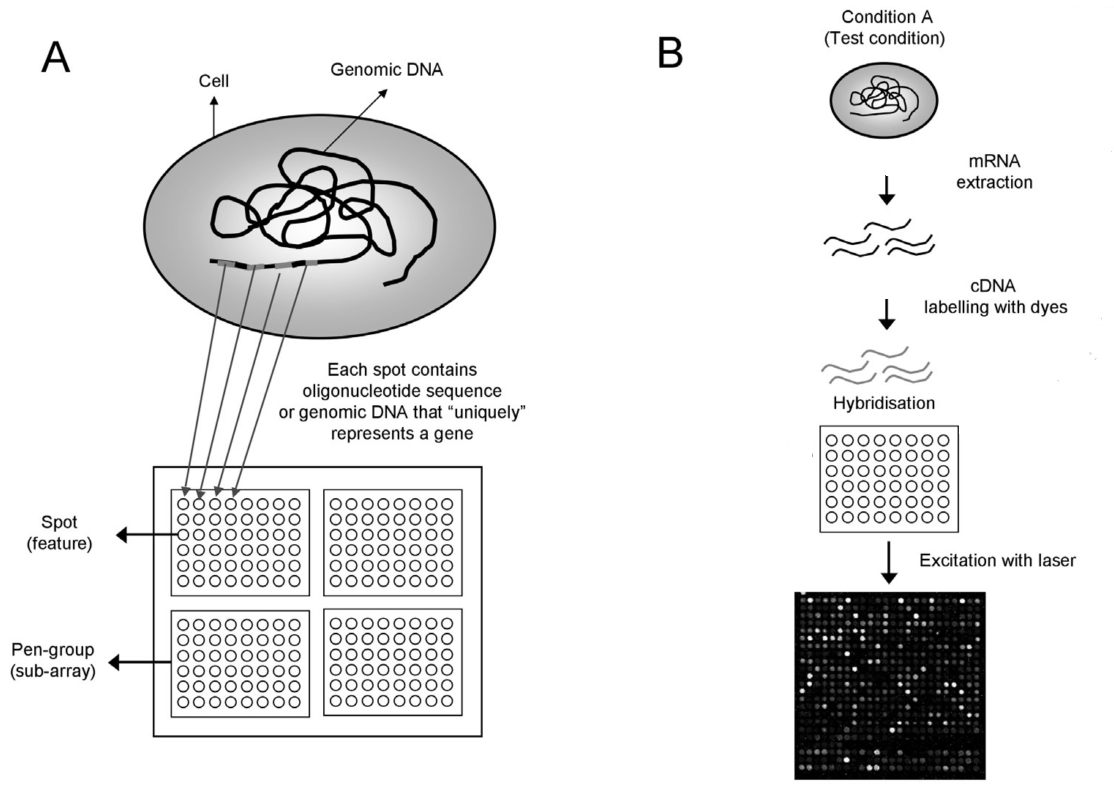
\includegraphics[width=0.8\textwidth]{micromatriz}
    \caption{Funcionamiento básico de una micromatriz de ADN \hl{Hacer esta figura nuevamente}}
    \label{fig:micromatriz}
\end{figure}
En las micromatrices de un solo canal, las moléculas de ARNm son extraídas de las células de interés del organismo y mediante diversas técnicas son transcritas inversamente a ADN. Luego, el ADN es transcrito nuevamente a ARNm utilizando ARN marcado con un compuesto fluorescente (biotina). Estas copias marcadas y aumentadas son luego colocadas en la micromatriz, permitiendo que el ARNm se difunda por toda la misma.\\
Cuando el ARNm encuentra una sonda que contiene su copia complementaria, se hibridiza con la misma, es decir se pega con una afinidad mucho mayor con la que se puede pegar a cualquier otra. Al lavarse la solución de ARNm, solo aquellos que se hibridizaron con la copia complementaria se mantienen unidos. Finalmente, se ilumina la micromatriz con luz laser de longitud adecuada y se mide la cantidad de fluorescencia emitida por cada sonda. Esta cantidad está asociada a la cantidad de ácido nucléico que se ligó a una dada sonda y eso a su vez será proporcional a la concentración de ese ARNm particular en el tejido de interés.\\
El resultado de un experimento con micromatrices es una tabla o matriz de expresión de $N_g x N_m$ donde cada fila corresponde a los niveles de expresión de cada gen particular ($N_g \approx 20000$ genes), y cada columna a cada muestra ($N_m \approx 15$ muestras) de tejido tomada.\\
Estos tecnologías plantean entonces el problema de como analizar bastas cantidades de datos para obtener información de interés, como ser:
\begin{enumerate}
	\item La identificación de los genes que forman parte de algún proceso biológico
	\item Agrupar tumores para su clasificación clínica
	\item Proveer evidencia de la función de proteínas cuyo rol en el organismo se desconoce
\end{enumerate}
En la actualidad, la aparición de tecnologías más rápidas y económicas de secuenciamiento, conocidas colectivamente como Next-generation sequencing (Secuenciamiento de próxima generación), están comenzando a dejar obsoleta la tecnología de micromatrices. Sin embargo, las mismas siguen siendo una herramienta útil en el estudio de los perfiles de expresión genética.\\
En este trabajo, analizaremos el dataset Wiegel, datos obtenidos mediante esta tecnología.\\
\hl{poner algo sobre Wiegel y si se uso single channel o doble channel}
\cite{Babu2004}
\cite{Schulze2001}
\cite{Domany2003}
\section{PIN - Redes de interacción de proteínas}
\label{sec:redes}
Las redes son construcciones útiles para esquematizar la organización de las interacciones en distinto tipo de sistemas. Las redes son particularmente valiosas a la hora de caracterizar interacciones interdependientes, es decir, interacciones tales que una interacción entre los componentes A y B, afectan las interacciones entre los componentes B y C y así sucesivamente.\\
La mayor parte de las funciones biológicas en una célula es llevada a cabo por proteínas a través de procesos de interacción entre ellas. Por lo tanto, es de fundamental importancia conocer no solo los niveles de expresión de una dada proteína, sino también, en simultaneo, las interacciones que lleva a cabo con otras proteínas. El registro en forma global de estas interacciones conforma lo que se denomina red de interacción de proteínas o PIN, y si la misma contempla la totalidad de las proteínas de una dada especie, la PIN correspondiente se conoce como interactoma completo.\\
\subsection{PIN AI1 y LCI binaria}
A lo largo de esta tesis se analizaron dos redes de interacción de proteínas con el objetivo de utilizarlas como referencia.\\
La primera, una red binaria de interacción de proteínas en todo el proteoma para la planta \textit{Arabidopsis thaliana} consistente en aproximadamente 5700 interacciones altamente confiables entre alrededor de 2700 proteínas, obtenida de \cite{Hahn2013}, material suplementario, tabla 4.\\
Para generar el interactoma, \cite{Hahn2013} utilizó una colección de aproximadamente 8000 marcos abiertos de lectura (secuencias de ARN comprendidas entre un codón de inicio de traducción y un codón de terminación) representando alrededor del 30\% de los genes codificantes. Probaron todas las interacciones de a pares con un método conocido como \textit{Sistema de doble híbrido} (Y2H por sus siglas en inglés), consistente en la activación de un gen reportero mediante la acción de un factor de transcripción sobre la secuencia regulatoria. Para ello, el factor de transcripción es separado en dos fragmentos, uno que reconoce la secuencia regulatoria y otro que promueve la activación de la transcripción. Estos dos fragmentos son luego conectados cada uno a cada una de las dos proteínas (llamadas carnada y presa) que se desean analizar. Si las dos proteínas interactúan entre si, el factor de transcripción se reconstituirá y se activará el gen reportero, visualizándose como crecimiento en un medio específico o una reacción con cambio de color.\cite{Bruckner2009}\\
Utilizando los pares obtenidos confeccionaron un conjunto de datos consistente en 5664 interacciones binarias entre 2661 proteínas, llamado Arabidopsis Interactome versión 1 ``main screen'', que llamaremos AI1.\\
\begin{figure}[h]
    \centering
    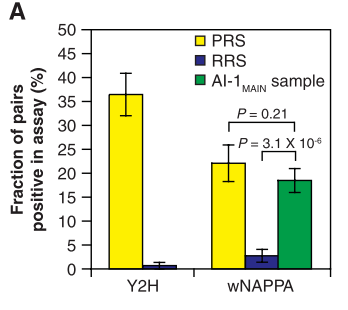
\includegraphics[width=0.4\textwidth]{calidad_ai1}
    \caption{Quality of AI-1MAIN.(A) Fraction of PRS, RRS, or AI-1MAIN sample pairs positive in Y2H or in wNAPPA at a scoring threshold of 1.5. Error bars, standard error of the proportion. P values, one-sided two-sample t tests (3). \hl{Ver si se puede poner esta figura, ver el epigrafe y como citarla}}
    \label{fig:calidad_ai1}
\end{figure}
La calidad de la red fue evaluada contra un conjunto de referencias positivas de 118 interacciones bien documentadas (PRS) y comparadas con un conjunto de referencia de 146 pares aleatorios de proteínas(RRS). Determinaron mediante la técnica de comparación \textit{wNAPPA}, que la fracción de interacciones reales en AI1, es decir su precisión, era de alrededor de 80\%, figura \ref{fig:calidad_ai1}. Esto implica que la red AI1 es una red de interacción de proteínas de alta calidad.\\
La segunda red utilizada fue una red binaria de interacción de proteínas, que llamaremos, $LCI_{binaria}$, obtenida de \cite{Hahn2013}, material suplementario, tabla 4, consistente en aproximadamente 4300 interacciones entre alrededor de 2200 proteínas de \textit{Arabidospis}. La misma fue obtenida mediante curado manual de literatura, es decir, en lugar de realizar ensayos de alto rendimiento en busca de pares de proteínas interactuantes, se realiza una revisión exhaustiva de la literatura existente en busca de interacciones que aparezcan en ensayos de pequeña escala previamente realizados sobre pocas proteínas y motivados por hipótesis previas (hypothesis-driven en inglés), ensayos altamente fiables.\cite{Cusick2009}\\
El solapamiento observado entre ambas se encuentra en el rango esperado dado la cobertura del proteoma que hacen estas redes, como muestra el diagrama de la figura \ref{fig:ai1_lci}.
\begin{figure}[h]
    \centering
    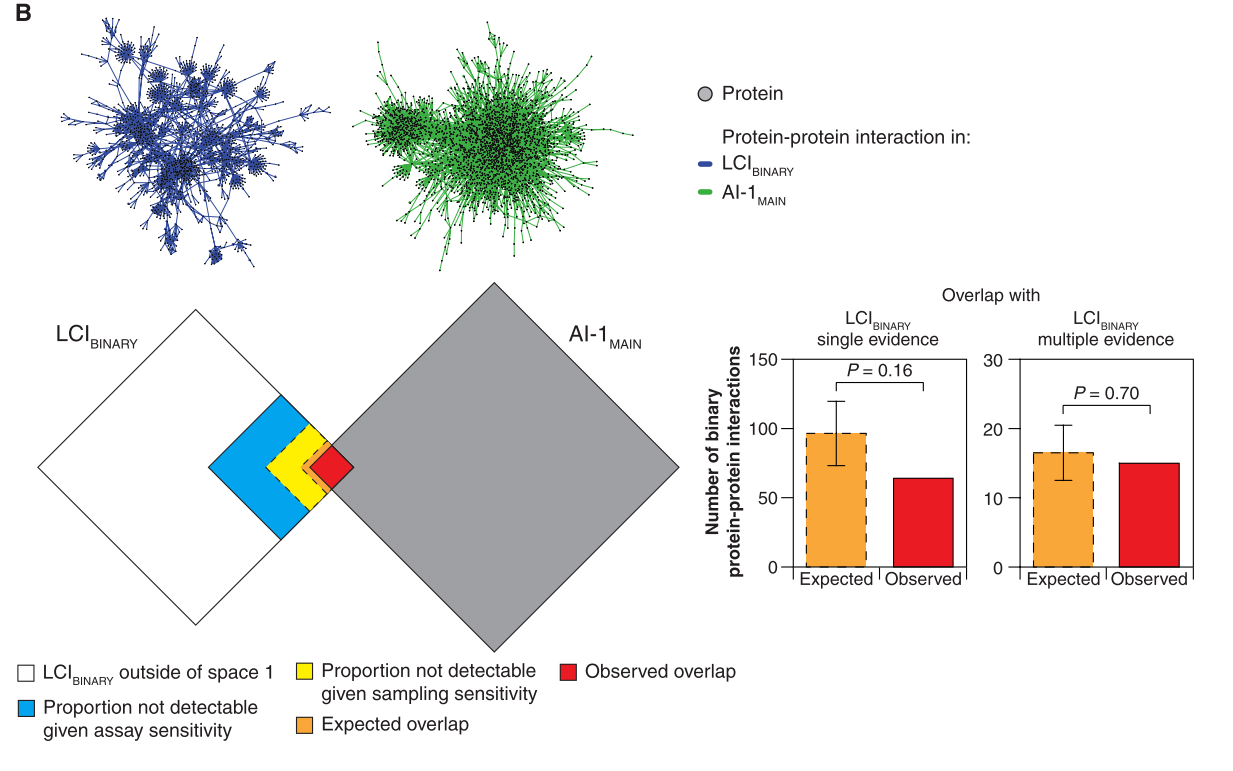
\includegraphics[width=0.8\textwidth]{ai1_lci}
    \caption{The number of literature-curated interactions recovered reflects AI-1MAIN framework parameters (6). (Top) Network rep- resentations of LCIBINARY and AI-1MAIN. (Bottom left) Data sets are represented by squared Venn diagrams; size is proportional to the number of interactions (3). (Bottom right) Observed and expected overlap given sensitivity and completeness of AI-1MAIN with LCIBINARY interactions supported by a single or multiple experimental evidences (3). PRS pairs were removed from LCIBINARY multiple evidence for this analysis. Error bars, two SD from the expected counts \hl{Ver si se puede poner esta figura, ver el epigrafe y como citarla}}
    \label{fig:ai1_lci}
\end{figure}
\section{KEGG - Vías metabólicas}
Los procesos celulares son llevados a cabo a través de interacciones entre varios genes y proteínas. Este tipo de actividades suele organizarse en vías, llamadas vías metabólicas, que consisten en grupos de genes que se coordinan para realizar una tarea específica. Son cadenas de reacciones bioquímicas que conducen de un sustrato inicial a uno o más productos finales. Descubrir este tipo de organizaciones es fundamental para obtener una imagen global de la actividad celular (figura \ref{fig:mapa_kegg}).\\
La Enciclopedia de Genes y Genomas de Kyoto (KEGG, por sus siglas en inglés), es una base de datos de recursos que comprenden funciones de alto nivel y utilidades de sistemas biológicos, como las células, los organismos y los ecosistemas, obtenida mediante información de nivel molecular generada por secuenciamientos de genoma y otros ensayos de gran escala. 
\begin{figure}[h]
    \centering
    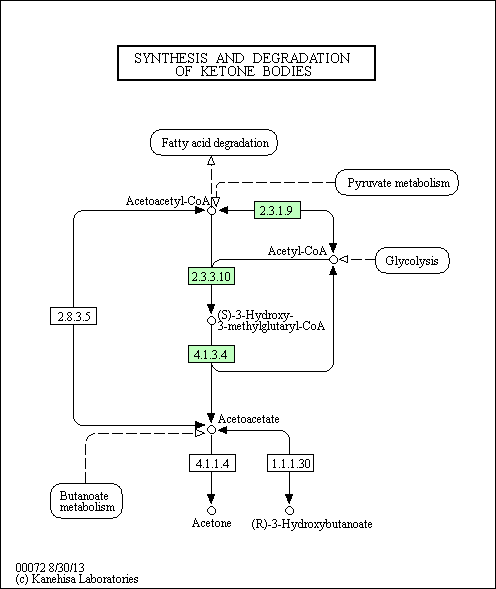
\includegraphics[width=0.8\textwidth]{mapa_kegg}
    \caption{Mapa KEGG de la vía metabólica de Arabidopsis Thaliana  \textit{Synthesis and degradation of ketone bodies} \hl{comentar mas o cambiar el idioma del grafico}}
    \label{fig:mapa_kegg}
\end{figure}
La misma provee de una base de datos de vías metabólicas que contiene recursos para la representación de procesos celulares tales como el metabolismo, transducción de señales y ciclo celular. En este trabajo utilizamos la base de datos KEGG de vías metabólicas de la planta \textit{Arabidospsis thaliana} disponible a través del paquete ``graphite'' (GRAPH Interaction from pathway Topological Environment) del lenguaje de programación R.\\
Se conformó una red uniendo todas las vías metabólicas presentes en la base de datos y teniendo en cuenta solamente aquellos genes presentes en el conjunto de datos Weigel.
\cite{Segal2003}\cite{Kanehisa2000}
\section{GO - Ontología genética}
Poder comparar y clasificar entidades es un mecanismo fundamental de las ciencias biológicas. El advenimiento de tecnologías de alta salida como las micromatrices de ADN, hace que sea necesario adoptar sistemas de representación del conocimiento que sean objetivos y estandarizados. Esto llevó al desarrollo de diversas ontologías para anotación de genes y de sus productos, y en particular, al desarrollo de la Ontología Génica (Gene ontology, GO por sus siglas en inglés).
El proyecto de Ontología Génica (GO) es un esfuerzo colectivo que intenta mantener un vocabulario y una descripción consistente de productos génicos a lo largo de distintas bases de datos. Esta ontología provee de un vocabulario controlado de términos definidos que representan las propiedades de los productos génicos (proteínas y secuencias de ARN, por ejemplo).\\
El proyecto GO consta de tres ontologías estructuradas que describen los productos génicos en terminos de sus procesos biológicos asociados (ontología \textit{Biological Process}, BP), de sus componentes celulares (ontología \textit{Cellular Component}, CC) y de sus funciones moleculares (ontología \textit{Molecular Function}, MF).\\
Un termino de un proceso biológico (BP) describe una serie de eventos realizados por uno o varios grupos de eventos moleculares con un comienzo y un fin definidos, por ejemplo, ``proceso celular fisiológico'' o ``transducción de señal''. Un proceso biológico no es equivalente a una vía metabólica ya que no intenta representar la dinámica o dependencias de la misma.\\
Un término de componente celular (CC) describe un componente de una célula que es parte de un objeto mayor, como ser una estructura anatómica (por ejemplo, retículo endoplasmático rígido, núcleo, etc.) o un grupo de productos génicos (por ejemplo, ribosoma, proteasoma, etc.).\\
Finalmente, los términos de función molecular (MF) describen las actividades que ocurren a nivel molecular, por ejemplo, ``actividad catalítica'' o ``actividad de transporte''.\\
La ontología GO está estructurada en tres grafos acíclicos dirigidos (DAG por sus siglas en inglés) independientes (uno para cada categoría ortogonal de productos génicos), donde cada nodo representa un término que describe alguna función. Los términos se unen entre si mediante relaciones del tipo ``es un'' o ``es parte de'', donde el primero expresa una relación de clase-subclase y el segundo una relación de parte-todo (figura \ref{fig:ejemplo_de_go}). Cuando un producto génico es descrito por un termino GO, se dice que el mismo está anotado en ese término, ya sea de forma directa o a través de herencia, ya que estar anotado en un término implica estar anotado en todos los términos ancestrales, regla conocida como \textit{regla del camino verdadero}.\\
\begin{figure}[h]
    \centering
    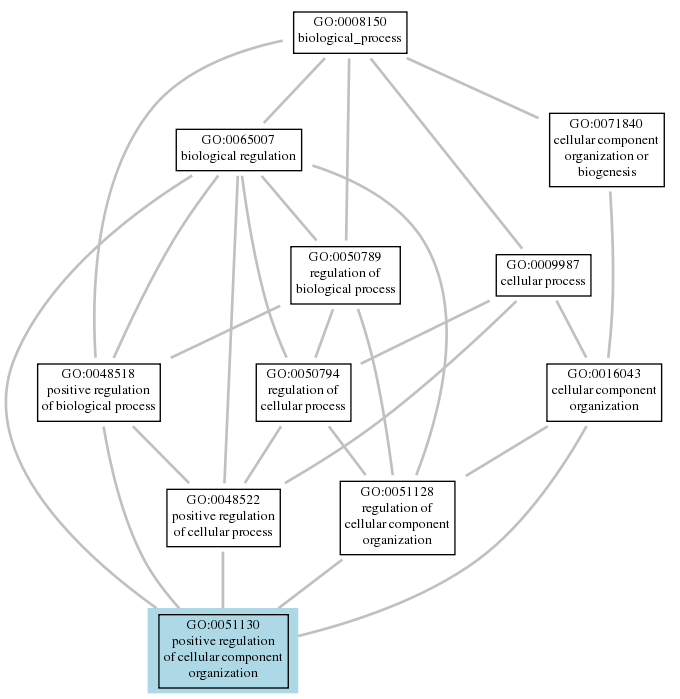
\includegraphics[width=0.5\textwidth]{ejemplo_de_go}
    \caption{Subgrafo mostrando el proceso biológico "Positive regulation" etc. \hl{poner nombres en castellano, flechas, etc}}
    \label{fig:ejemplo_de_go}
\end{figure}
Formalmente, podemos describir estás relaciones de la ontología GO de la siguiente manera:\\
Sea $C=\{c_i / 1\leq i \leq N\}$ un conjunto ordenado finito de conceptos que representan términos GO. Los mismos se relacionan entre si a través de las relaciones antes consignadas, de tal forma que $c_i \rightarrow c_j$ denota que $c_i$ es un/es parte de $c_j$. Basado en esto, es posible definir una relación binaria sobre $C$, denotada por $\preceq$, tal que $c_i \preceq c_j$, es decir $c_j$ es un ancestro de $c_i$ en la jerarquía GO. Notar entonces que si $c_k \preceq c_i$ y $c_i \preceq c_j \Rightarrow c_k \preceq c_j$ (regla del camino verdadero). En cada grafo existe un término raíz de la jerarquía $r$, tal que $c_i \preceq r \forall c_i \in C$.\\
Los conceptos más generales se hallarán más próximos al término raíz, mientras que los más específicos e informativos se alejarán del mismo. La anotación de un gen o producto génico se realiza siempre al nodo mas especifico, pudiendo ser anotado además en varios conceptos biológicos a la vez.\\
Una anotación en GO consiste en un término GO junto con una referencia que describe el tipo de trabajo o análisis que se realizó para asociar un gen con un término específico. Cada anotación debe además incluir un código de evidencia que indica la forma en que se justifica la anotación a un término particular, lo que le confiere un grado de fiabilidad.\\En particular, existen dos grupos de anotaciones, aquellas que fueron curadas manualmente y aquellas que fueron inferidas de anotaciones electrónicas (IEA). Este último tipo de anotaciones funcionales se realiza de forma automatizada sin que intermedie un curador e involucran comparaciones por similitud de secuencia o anotaciones transferidas de bases de datos y por lo tanto poseen una baja calidad y una gran cobertura, formando alrededor del 40\% de las anotaciones totales. Además, dentro del grupo de las anotaciones que fueron curadas manualmente, se tienen aquellas que fueron inferidas por medio de experimentos (IDA, IEP, IGI, IMP, IPI), aquellas que fueron inferidas por medio de análisis computacional (IBA, ISS, RCA, ISM). La figura \ref{fig:codigos_de_evidencia} muestra la fracción que representa cada tipo de anotación para cada ontología.
\begin{figure}[h]
    \centering
    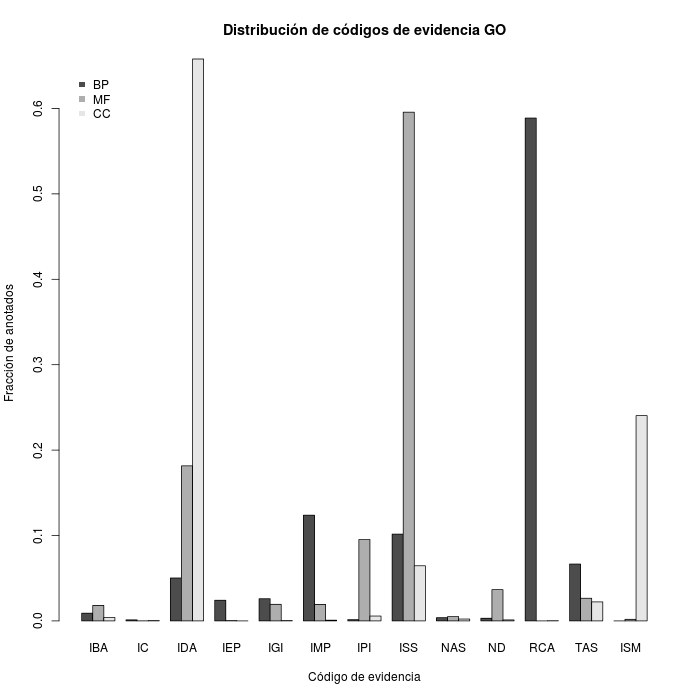
\includegraphics[width=0.8\textwidth]{codigos_de_evidencia}
    \caption{Códigos de evidencia en cada una de las ontologías y la fracción del total que representan. \hl{comentar mas}}
    \label{fig:codigos_de_evidencia}
\end{figure}
Las cantidad total de anotaciones para BP, MF y CC, sin tener en cuenta aquellas pertenecientes a la categoría IEA, totalizan 2540816, 207087 y 1043851 anotaciones respectivamente.\\
En particular, en este trabajo se tuvieron en cuenta únicamente las evidencias obtenidas experimentalmente. Para ello, se tomaron dos subconjuntos de anotaciones de la ontología BP, que llamaremos BPA, consistente en las anotaciones IDA, IPI, IGI, IMP, con un total de 512235 anotaciones y BPB, consistente en las anotaciones IDA, IPI, IGI, IMP y IEP, con un total de 573688. Además, se utilizó un subconjunto de la ontología CC, consistente en las anotaciones IDA, IPI, IGI, IMP, con un total de 693991 anotaciones.\cite{Pandey2008} \cite{Resnik1995} \cite{Bose2016} \cite{Pesquita2009} \cite{Berenstein2014} \cite{Ashburner}

\chapter{Métodos de agrupamiento de datos}
Un método de agrupamiento de datos o método de ``clustering'', es un método de clasificación no supervisado que permite la partición de un conjunto de $N$ objetos en $K$ grupos o clases, de tal forma que los objetos miembro de un grupo sean más similares entre si (en algún sentido a definir) que entre los miembros de otros grupos.\\\\
Son métodos no supervisados ya que en un proceso de agrupación no existen clases definidas previamente ni ejemplos de que tipo de relaciones se desea encontrar entre los objetos, por lo que el mismo proceso debe generar las clases iniciales a las cuales asignar los objetos en el proceso de clasificación.\\\\
Estas técnicas permiten el descubrimiento o identificación de distribuciones y patrones subyacentes en los datos, posibilitando obtener conclusiones sobre los mismos, lo que las hace una de las herramientas más útiles en procesos de minería de datos y aprendizaje automatizado en campos tan diversos como las ciencias sociales, las ciencias médicas y la ingeniería.\\\\
Dependiendo de los criterios utilizados para realizar la partición, un proceso de agrupamiento puede resultar en diferentes particiones. Como ejemplo de esto podemos tomar el conjunto de números $\{-5, -3, -2, 2, 3\}$. Si decidimos agruparlos por su módulo, obtendremos los conjuntos $\{-5\}$, $\{-3, 3\}$, $\{-2, 2\}$, mientras que si decidimos agruparlos por positividad o negatividad, obtendremos los conjuntos $\{-5, -3, -2\}$ y $\{2, 3\}$. También podríamos haber optado por agrupar por paridad, si son o no primos, etc. Como se observa de un ejemplo tan sencillo, es de fundamental importancia la elección de las propiedades de los objetos a partir de las cuales realizar el agrupamiento.\\\\
En el presente trabajo nos interesará agrupar y caracterizar conjuntos de genes de un organismo modelo, la planta \textit{Arabidopsis thaliana}, en base a sus perfiles de expresión génica a lo largo de los diversos tratamientos presentados en el capitulo anterior.\cite{Gan2007, Halkidi2001, Domany1999}\\\\
Discutiremos a continuación diferentes metodologías y criterios de similaridad que pueden ser considerados para ello.
\section{Similaridad, distancia y disimilaridad}
Las distancias y similaridades tienen un rol preponderante en el análisis de agrupamiento de datos y por regla general son conceptos recíprocos.\\\\
Una medida de similaridad o coeficiente de similaridad se utiliza para indicar de forma cuantitativa la fuerza de la relación entre dos objetos del conjunto. Los $i = 1, 2, ...N$ objetos de un conjunto $E$ pueden ser definidos en términos de las coordenadas $\vec{Xi}$ de sus puntos representativos en un espacio $n-dimensional$. Sean $\vec{x}=\{x_0, x_1,...,x_n\}$ e $\vec{y}=\{y_0, y_1,...,y_n\}$ dos puntos $n-dimensionales$. Entonces, el coeficiente de similaridad entre ambos será una función de sus atributos:
\begin{equation}
	s(\vec{x}, \vec{y}) = s((x_0, x_1,...,x_n), (y_0, y_1,...,y_n))
\end{equation}
con $s$ una función simétrica, es decir, $s(\vec{x}, \vec{y}) = s(\vec{y}, \vec{x})$. Cuanto mayor es el coeficiente de similaridad, mayor es la similaridad entre ambos.\\\\
Por otro lado, las medidas de disimilaridad o de distancia se comportan de forma inversa, a mayor distancia o disimilaridad, más diferentes son dos puntos.
Una métrica de distancia es una función $d \in R$ definida sobre un conjunto $E$ que cumple las siguientes propiedades:
\begin{enumerate}
\item No-negatividad: $d(\vec{x}, \vec{y}) \geq 0$
\item Reflexividad: $d(\vec{x}, \vec{y}) = 0 \iff \vec{x} = \vec{y}$
\item Conmutatividad: $d(\vec{x}, \vec{y}) = d(\vec{y}, \vec{x})$
\item Desigualdad triangular: $d(\vec{x}, \vec{y}) \leq d(\vec{x}, \vec{z}) + d(\vec{z}, \vec{y})$
\end{enumerate}
con $\vec{x},\vec{y},\vec{z}$ objetos arbitrarios del conjunto.\\\\

Una medida de disimilaridad es una métrica si cumple con las propiedades antes enunciadas. \\\\
Aunque no pareciera existir una definición formal de métrica de similaridad, Chen y colaboradores definen en \cite{Chen2009} una métrica de similaridad como una función $s$ que cumple:
\begin{enumerate}
\item $s(\vec{x}, \vec{y}) = s(\vec{y}, \vec{x})$
\item $s(\vec{x}, \vec{x}) \geq 0$
\item $s(\vec{x}, \vec{x}) \geq s(\vec{x}, \vec{y})$
\item $s(\vec{x}, \vec{x}) = s(\vec{y}, \vec{y}) = s(\vec{x}, \vec{y}) \iff x=y$
\item $s(\vec{x}, \vec{y}) + s(\vec{y}, \vec{z}) \leq s(\vec{x}, \vec{z}) + s(\vec{y}, \vec{y})$
\end{enumerate}
La condición 5 indica que la similaridad entre $\vec{x}$ y $\vec{z}$ a través de $\vec{y}$ no es mayor que la similaridad directa entre $\vec{x}$ y $\vec{z}$ sumada a la autosimilaridad de $\vec{y}$. Esta propiedad es el equivalente de la desigualdad triangular para una distancia métrica.\\\\
Si bien es deseable que una similaridad o disimilaridad sea una métrica, existen muchas medidas de similaridad o disimilaridad que dan excelentes resultados en técnicas de agrupamiento de datos sin ser métricas, es decir, sin que necesariamente cumplan la desigualdad triangular o el item 5 de métrica de similaridad.\cite{Chen2009}\\\\
Finalmente, los objetos del conjunto pueden ser especificados por medio de una ``matriz de distancia'' de $N\times N$ cuyos elementos $d_{ij}$ indican la disimilaridad entre los puntos $i$ y $j$.\cite{Halkidi2001, Domany1999, Gan2007, Kheng2010}

\subsection{Medidas de distancia}
El análisis de datos de expresión génica se basa principalmente en la comparación de perfiles de expresión génica. Para poder comprarlos, se requiere una medida que cuantifique cuán similares o disimilares son los objetos considerados. La elección de una medida de distancia será entonces de fundamental importancia para lograr agrupamientos que tengan sentido en el contexto de los datos analizados. En las subsiguientes secciones se listarán las medidas de distancia más comúnmente utilizadas en el agrupamiento de datos (no necesariamente de datos de perfiles de expresión).
\subsubsection{Distancia euclidiana}
La distancia euclidiana es probablemente la distancia más utilizada en el contexto de datos numéricos.\\
Para dos puntos $\vec{x}$ e $\vec{y}$ en un espacio $n-dimensional$, la distancia euclidiana se define como:
\begin{equation}
	d_{euc}(\vec{x}, \vec{y}) = [\sum\limits_{i=1}^n (x_i-y_i)^2]^\frac{1}{2} = [(\vec{x}-\vec{y})(\vec{x}-\vec{y})^T]^\frac{1}{2}
\end{equation}
con $x_i$ e $y_i$ los valores de la \textit{i}esima componente de $\vec{x}$ e $\vec{y}$ respectivamente.

\subsubsection{Distancia Manhattan o Taxicab}
La distancia Manhattan o taxicab es llamada así por ser la distancia que debería recorrer un taxi en una ciudad para ir de un punto a otro, suponiendo la ciudad como una cuadrícula perfecta.\\
Para dos puntos $\vec{x}$ e $\vec{y}$ en un espacio $n-dimensional$, la distancia Manhattan se define como:
\begin{equation}
	d_{man}(\vec{x}, \vec{y}) = \sum\limits_{i=1}^n |(\vec{x}-\vec{y})|
\end{equation}
\subsubsection{Distancia máxima}
Para dos puntos $\vec{x}$ e $\vec{y}$ en un espacio $n-dimensional$, la distancia máxima se define como:
\begin{equation}
	d_{max}(\vec{x}, \vec{y}) = \max_{1 \leq j \leq n} |x_i-y_i|
\end{equation}
\subsubsection{Distancia de Minkowsky}
Para dos puntos $\vec{x}$ e $\vec{y}$ en un espacio $n-dimensional$, la distancia de Minkowsky se define como:
\begin{equation}
	d_{mink}(\vec{x}, \vec{y}) = [\sum\limits_{i=1}^n (x_i-y_i)^r]^\frac{1}{r}, r \geq 1
\end{equation}
$r$ es el orden de la distancia de Minkowsky. Notar que si tomamos $r = 2,1,\inf$ obtenemos la distancia euclidiana, la Manhattan y la máxima, respectivamente.
\subsubsection{Coeficiente de correlación de Pearson}
Una de las métricas más utilizadas para medir similaridad entre perfiles de expresión, como los presentados en la figura \ref{fig:perfiles_sin_agrupar}, es el coeficiente de correlación de Pearson \cite{Babu2004}.\\\\
El coeficiente de correlación fue desarrollado por Karl Pearson basado en ideas introducidas por Francis Galton alrededor del año 1880.\\\\
\begin{figure*}[t!]
    \centering
    \begin{subfigure}[t]{0.6\textwidth}
    \centering
    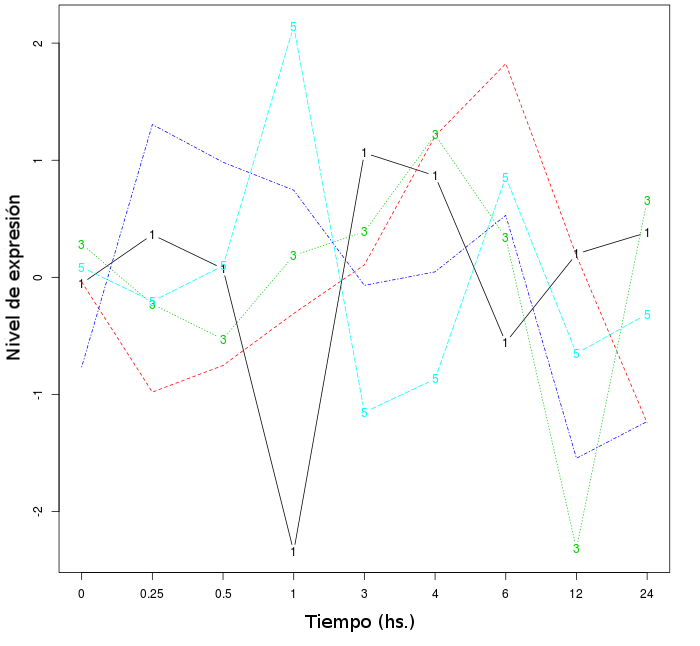
\includegraphics[width=1\textwidth]{perfiles_sin_agrupar}
    \caption{Perfiles de expresión de cinco genes tomados al azar.}
    \label{fig:perfiles_sin_agrupar}
    \end{subfigure}    
    
    \begin{subfigure}[t]{0.45\textwidth}
    \centering
    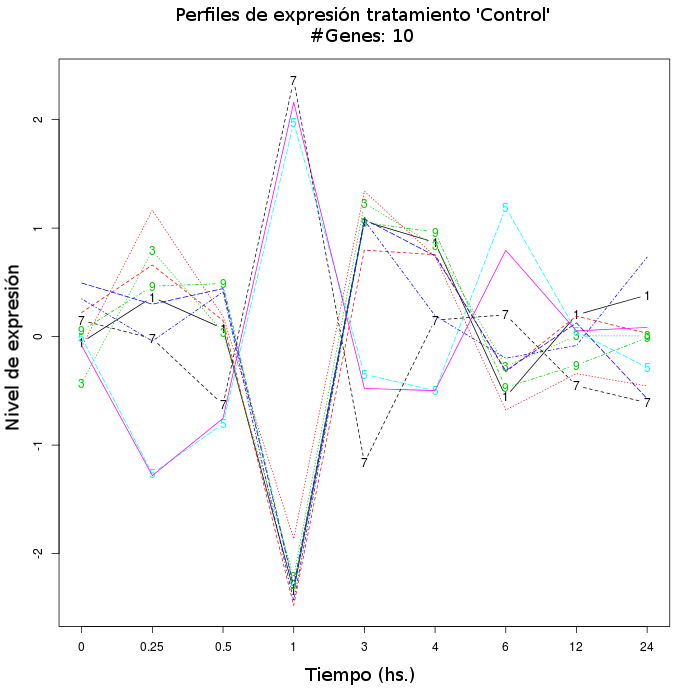
\includegraphics[width=1\textwidth]{perfiles_anti_coregulados}
    \caption{Perfiles de expresión de 10 genes que están co-expresados y anti co-expresados.}
    \label{fig:perfiles_anti_coregulados}
    \end{subfigure}
    \begin{subfigure}[t]{0.45\textwidth}
    \centering
    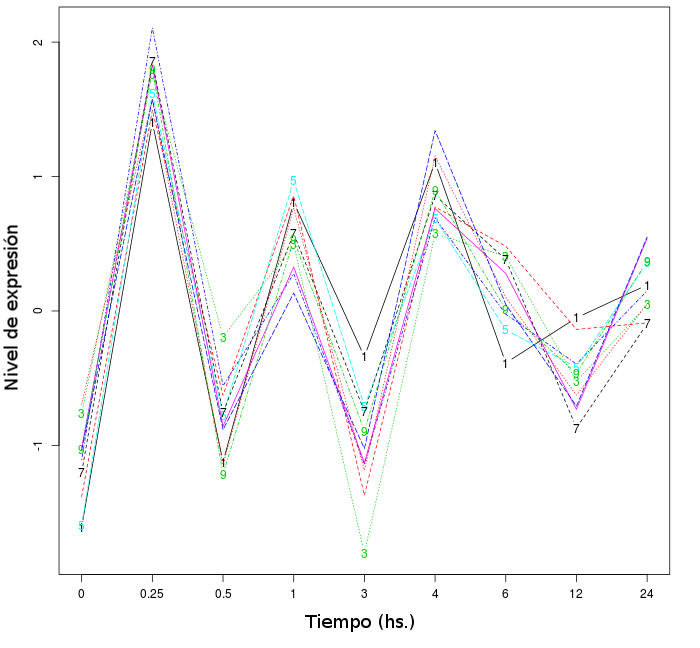
\includegraphics[width=1\textwidth]{perfiles_coregulados}
    \caption{Perfiles de expresión de 10 genes que están co-expresados.}
    \label{fig:perfiles_coregulados}
    \end{subfigure}
    \caption{Distintos grupos de perfiles de expresión para el tratamiento \textit{Control}. Cada gen está representado por un color y un número. Cada punto indica una medición del nivel de expresión del gen. Los puntos están unidos por lineas para mejorar su visualización.}
\end{figure*}
Para dos puntos $\vec{x}$ e $\vec{y}$ en un espacio $n-dimensional$, representando el perfil de expresión de dos genes a lo largo de un dado tratamiento, el CCP se define como:
\begin{equation}
	r(\vec{x}, \vec{y}) = \frac{\sum\limits_{i=1}^n(x_i-\bar{x})(y_i-\bar{y})}{[\sum\limits_{i=1}^n(x_i-\bar{x})^2]^\frac{1}{2}[\sum\limits_{i=1}^n(y_i-\bar{y})^2]^\frac{1}{2}}
	\label{eq:ccp}
\end{equation}
o de forma equivalente:
\begin{equation}
	r(\vec{x}, \vec{y}) = \frac{\frac{1}{n-1}\sum\limits_{i=1}^n(x_i-\bar{x})(y_i-\bar{y})}{s_x s_y}
\end{equation}
con $s$ la desviación estandar de la muestra. El centrar alrededor de la media permite comparar la forma de ambos perfiles, en lugar de su magnitud.\\\\
Valores altos de $r$ implican que las fluctuaciones respecto de la media de las respectivas componentes se encuentran ``en sincronia''. En caso de no estarlo el valor esperado tiende a cero. Finalmente si las fluctuaciones tienden a ocurrir ``sincronizadamente'' pero en sentidos opuestos $r \Rightarrow -1$.\\\\
En nuestro caso, $r=+1$ corresponde a genes que estan siendo coexpresados por la maquinaria celular, mientras que $r=-1$ a genes anti-coexpresados. En el primer caso los perfiles de ambos genes
(apropiadamente reescaleados) coinciden perfectamente, mientras que en el segundo son perfectamente opuestos.\\\\
La correspondiente medida de distancia puede ser calculada como \cite{Dhaeseleer2005}:
\begin{equation}
	d_{ccp}(\vec{x}, \vec{y}) = 1-r(\vec{x}, \vec{y})
	\label{eq:distancia_correlacion}
\end{equation}
o alternativamente:
\begin{equation}
	d_{ccp}(\vec{x}, \vec{y}) = 1-|r(\vec{x}, \vec{y})|
	\label{eq:distancia_correlacion_absoluta}
\end{equation}
En el caso de la distancia definida en \ref{eq:distancia_correlacion_absoluta}, al tomar el valor absoluto del CCP, genes cuyos perfiles son iguales pero opuestos (están anti-coexpresados) pueden encontrarse más cerca en el sentido de $d_{ccp}$ que aquellos que son expresados hacia arriba o abajo pero en distintas magnitudes. Por lo tanto, esta distancia permite encontrar grupos de genes que son coexpresados, sin importar en que sentido (Figura \ref{fig:perfiles_anti_coregulados}) sean coexpresados.
En el caso de la distancia definida en \ref{eq:distancia_correlacion}, solamente se consideran cercanos aquellos genes cuyos perfiles sean coexpresados o bien hacia arriba o bien hacia abajo (Figura \ref{fig:perfiles_coregulados}).\cite{Hennig2013, Kheng2010, Babu2004, Gan2007}\\\\
En el presente trabajo se utilizará como distancia la definida en \ref{eq:distancia_correlacion} para encontrar grupos de genes que únicamente se hayan coexpresado o bien hacia arriba o bien hacia abajo.\cite{Eisen1998}
\clearpage
\subsection{Similaridad semántica}
La adopción de ontologías provee los medios para comparar aspectos de entidades que de otra forma no podrían ser comparados. Por ejemplo, si dos productos génicos son anotados dentro del mismo esquema, es posible compararlos mediante el análisis de los términos en los cuales están anotados de forma explícita utilizando medidas de similaridad semántica. Se define una medida de similaridad semántica como una función tal que dados dos términos de la ontología o un conjunto de términos en los que dos genes están anotados, la función devuelve un escalar que refleja la cercanía de sentido entre ellos.\\\\
Es posible cuantificar la similaridad semántica en una ontología representada por un grafo como GO, mediante diversas estrategias.
\subsubsection{Comparación de términos en GO}
Sea $C$ el conjunto de todos los términos de una ontología GO, con un número total $\#C$ de anotaciones. Un término $c_i$ tendrá $\#c_i$ anotaciones, ya sea directamente o por intermedio de cualquiera de sus hijos. La probabilidad de que un gen tomado al azar, sin otro tipo de información, se encuentre anotado al concepto $c_i$ será entonces $P(c_i) = \frac{\#c_i}{\#C}$, con $P:C\Rightarrow [0,1]$.\\\\
Se define el contenido de información de $c_i$ como $IC = -log_2(P(c_i))$, cantidad en el intervalo $(0, -log_2[\frac{1}{\#C}])$, que indica cuán específico e informativo es un término de la ontología. Para un $c_i$ y $c_j$ tales que $c_i \preceq c_j$, se tiene que $IC(c_i) \geq IC(C_j)$. Cuanto más específico sea un término, es menos probable que un gen dado esté anotado en el mismo, y por lo tanto, su contenido de información es mayor. El nodo raíz de la ontología tiene un contenido de información nulo, ya que es el ancestro de todos los términos de la misma y por lo tanto, saber que un concepto está anotado a la raíz no aporta información.\\\\
Es posible definir una medida entre pares de términos utilizando el IC. Una de las medidas de similaridad semántica más comúnmente utilizadas es la medida de similaridad semántica introducida por Resnik en \cite{Resnik1995}, que consiste en asignar como la medida de similaridad entre dos términos, el contenido de información del ancestro en común más informativo (el MICA):
\begin{equation}
	Sim_{res}(c_i, c_j) = \max\limits_{c \in S(c_i, c_j)}(-log_2[P(c)]) = IC(MICA[c_i, c_j])
\end{equation}
Con $S(c_i, c_j)$ el conjunto de ancestros comunes de $c_i$ y $c_j$. De esta manera, para cuantificar la información compartida (y estimar entonces su similaridad semántica) se considera el contenido de información de los ancestros en común que dos términos poseen.\\\\
A modo de ejemplo, tomemos el DAG de la figura \ref{fig:dag}, con 9 términos o conceptos: $C=\{R, c_0,...,c_7\}$ y con 5 entidades mapeadas (genes anotados): $g_1=\{5, 6, 2, 0, r\}$, $g_2=\{5, 4, 2, 3, 0, r\}$, $g_3=\{7, 1, r\}$, $g_4=\{4, 3, 0, r\}$ y $g_5=\{2, 0, r\}$. Podemos calcular la similaridad semántica de Resnik entre los términos $c_4$ y $c_5$, por ejemplo, sabiendo que $\#C = 5$ y que el ancestro común más informativo de ambos es $c_0$, con $\#c_0=4$. Se tiene entonces que $Sim_{res}(c_4, c_5) = IC(MICA) = IC(c_0) = -log_2(\frac{\#c_0}{\#C}) = -log_2(\frac{4}{5}) = 0.32$. Si quisieramos calcular ahora la similaridad semántica Resnik entre $c_5$ y $c_6$, obtendríamos $Sim_{res}(c_5, c_6) = IC(c_2) = -log_2(\frac{3}{5}) = 0.73$. Por lo tanto, para Resnik, los conceptos $c_5$ y $c_6$ son entre sí, más similares que los conceptos $c_4$ y $c_5$.\\\\
\begin{figure}[h]
    \centering
    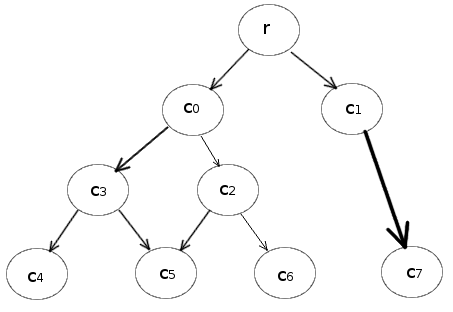
\includegraphics[width=0.5\textwidth]{dag}
    \caption{DAG con 9 términos o conceptos: $C=\{R, c_0,...,c_7\}$ y con 5 entidades mapeadas (genes anotados): $g_1=\{5, 6, 2, 0, r\}$, $g_2=\{5, 4, 2, 3, 0, r\}$, $g_3=\{7, 1, r\}$, $g_4=\{4, 3, 0, r\}$ y $g_5=\{2, 0, r\}$}
    \label{fig:dag}
\end{figure}
Existen más de dos docenas de medidas de similaridad entre términos GO, y no siempre es claro cuál es el mejor para un dado propósito. Sin embargo, generalmente la elección de una medida por defecto es suficiente\cite{Bose2016}. En este trabajo utilizaremos la $Sim_{res}$, por tratarse de una medida simple y efectiva.\\\\
Una vez establecida una medida de similaridad semantica entre termino GO, existen distintas formas para extender esta idea y definir una similaridad semántica entre genes. Básicamente existen 2
estrategias. La primera se basa en medidas globales (groupwise en inglés), que comparan globalmente los conjuntos de términos en los que dos genes están anotados, $GO(g_1)$ y $GO(g_2)$, por ejemplo, contando cuantos términos comparten: $|GO(g_1) \cap GO(g_2)|$.\cite{Lee2004} \\\\
La segunda estrategia se basa en medidas de a pares (pairwise en inglés), calculando la similaridad semántica término a término de cada uno de los conjuntos $GO(g_1)$ y $GO(g_2)$ y luego aplicando sobre esta similaridad alguna operación para obtener una medida de similaridad entre estos genes.\\\\
El primer paso para esto es calcular una matriz de similaridad $S$ de $N\times M$ que contenga la similaridad de a pares, entre todos los pares de términos de estos conjuntos, con $N=|GO(g_1)|$ y $M=|GO(g_2)|$, utilizando alguna de las medidas de similaridad semántica entre términos, por ejemplo, $Sim_{res}$:

\begin{equation}
	S(g_1, g_2)_{ij} = Sim(GO(g_1^i), GO(g_2^j)), \forall i \in \{1,...,N\} y \forall j \in \{1,...,M\}
\end{equation}
Notar que esta matriz puede no ser simétrica.\\\\
Cada una de las $N$ filas corresponde a la similaridad entre la anotación $i-esima$ del gen $1$ y todas las $M$ anotaciones del gen $2$ y cada una de las $M$ columnas corresponde a la similaridad entre la anotación $j-esima$ del gen $2$ y todas las $N$ anotaciones del gen $1$.\\\\
A partir de $S_{ij}$ es posible definir tres métodos para obtener una medida de similaridad entre genes.
El primer método, propuesto en \cite{Sevilla2005}, consiste en tomar como similaridad, la máxima similaridad entre todos los términos:
\begin{equation}
	Sim_{max}(GO(g_i), GO(g_j)) = \max\{S_{ij}\}
\end{equation}
El segúndo método, propuesto en \cite{Lord2003}, consiste en tomar el valor medio de todos los valores de la matriz $S_{ij}$:
\begin{equation}
	Sim_{med}(GO(g_i), GO(g_j)) = \frac{1}{N.M}\sum\limits_{i,j}S_{ij}
\end{equation}
Finalmente, el tercer método, propuesto en \cite{Pesquita2009}, implica tomar el valor medio de los máximos de cada fila, el valor medio de los máximos de cada columna, y quedarse con el máximo de esos dos valores. Este criterio de similaridad se conoce como \textit{rcmax}:
\begin{equation}
	Sim_{rcmax}(GO(g_1), GO(g_2)) = \max\{\frac{1}{N}\sum\limits_{i}\max\limits_{1\leq j \leq M}S_{ij}, \frac{1}{M}\sum\limits_{j}\max\limits_{1\leq i \leq N}S_{ij}\}
	\label{eq:sim_rcmax}
\end{equation}
Como muchos genes están anotados en conceptos muy diversos por participar en procesos biológicos muy distintos, e incluso puede haber genes que no están anotados en ningún concepto, la medida de similaridad $Sim_{med}$ tiende a dar valores más bajos que otros métodos. Por el contrario, la medida $Sim_{max}$ tiende a dar valores más altos, por ser una medida más optimista. En este trabajo utilizaremos el tercer método, $Sim_{rcmax}$, por ser un compromiso entre ambos casos extremos.
\cite{Resnik1995, Pesquita2009, Bose2016, Lin1998, Jiang1997, Sevilla2005, Lord2003}

\section{Estrategias de agrupamiento}
En la sección anterior abordamos distintas metodologías para cuantificar la noción de similaridad en diversos espacios.\\\\
En lo que sigue introduciremos las diferentes estrategias de agrupamiento de datos utilizadas en este trabajo, tanto para agrupamiento de perfiles transcripcionales como de armado de comunidades en las redes presentadas anteriormente.\\\\
Es posible distinguir dos tipos de agrupamientos, conocidos como agrupamiento duro (hard clustering en inglés), y agrupamiento difuso (fuzzy clustering en inglés). En el primer caso, el de agrupamiento duro, cada objeto del conjunto de datos es asignado a un y solo un grupo, mientras que en el segundo caso, el de agrupamiento difuso, un elemento del conjunto puede pertenecer a varios grupos, con distinta probabilidad. En este trabajo utilizaremos únicamente métodos de agrupamiento duro.\\\\
\section{Agrupamientos no jerárquicos}
\label{sec:agrupamientos_no_jerarquicos}
Además de la distinción mencionada más arriba, los métodos de agrupamiento pueden dividirse (entre otros) fundamentalmente entre agrupamientos jerárquicos y agrupamientos no jerárquicos.
Las dos estrategias de agrupamientos no jerárquicos que se presentan a continuación fueron utilizadas en el desarrollo de este trabajo.
\subsection{K-means}
K-means es un método usual de agrupamiento no jerárquico en donde cada observación pertenece al grupo con la media más cercana a la observación, y donde $K$, el número de grupos, debe ser fijado a priori y puede ser determinado arbitrariamente o estimado a partir de algún factor de merito apropiado.\cite{Hartigan1979}\\\\
Más formalmente, sea un conjunto de observaciones $\{\vec{x_1},...,\vec{x_n}\}$, k-means construye una partición de las observaciones en $k$ grupos con $k \leq n$ a fin de minimizar una función de costo, como ser la suma de los cuadrados dentro de cada grupo $G = \{g_1,...,g_k\}$: 
\begin{equation}
	C = argmin\sum\limits_{i=1}^k \sum\limits_{x_j \in g_i}||x_j-\mu_i||^2
\end{equation}
Con $\mu_i$ el valor medio de los elementos del grupo $g_i$.
La figura \ref{fig:ejemplo_k_means} muestra un conjunto de observaciones y los grupos que se obtienen fijando $k=2$ y $k=5$, junto con sus respectivos centroides.
\begin{figure}[h]
    \centering
    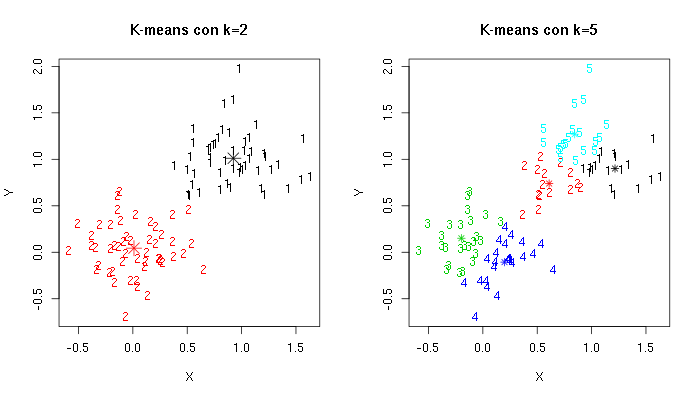
\includegraphics[width=0.8\textwidth]{ejemplo_k_means}
    \caption{Agrupamiento de ejemplo para un conjunto de puntos bidimensionales aleatorios utilizando k-means con $k=2$ y $k=5$. Cada punto está representado por un número y un color indicando su grupo de pertenencia.}
    \label{fig:ejemplo_k_means}
\end{figure}
Se observa que dependiendo del $k$ utilizado, el algoritmo encuentra particiones con mayor o menor nivel de \textit{resolución}. Volveremos sobre el tema de la resolución más adelante.
\cite{Kogan2006}

\subsection{PAM}
Si bien k-means es uno de los métodos de partición más utilizados ya que es muy eficiente en términos de tiempo computacional, el mismo es muy sensible a observaciones aisladas. Por esta razón, en algunos métodos se reemplazan los centroides, que son puntos no necesariamente pertenecientes al conjunto de observaciones, por medoides, que son los objetos más centrales dentro del grupo (se reemplaza k-means por k-medoids). Esto hace que el método sea insensible a observaciones aisladas.\\\\
Particionar alrededor de medoides (Partitioning around medoids en inglés) es uno de los métodos más conocidos que hace uso de este concepto, buscando minimizar la función de costo:
\begin{equation}
	C = argmin\sum\limits_{i=1}^k \sum\limits_{x_j \in g_i} d(x_j, m_i)
\end{equation}
Con $m_i$ el medoide del grupo $i$ y $d(x_j, m_i)$ la distancia entre el objeto $x_j$ del grupo $i$ y el medoide del mismo grupo.
\cite{Park2009, Ibrahim2012}
\section{Agrupamientos jerárquicos}
Existen dos acercamientos distintos para realizar un agrupamiento jerárquico: se puede ir ``desde abajo hacía arriba'', agrupando grupos más chicos en grupos más grandes, lo que se conoce como agrupamiento aglomerativo, o se puede ir ``desde arriba hacia abajo'', dividiendo grupos más grandes en grupos más chicos, lo que se conoce como agrupamiento divisivo. En este trabajo nos interesará únicamente trabajar con agrupamientos aglomerativos.\\\\
Un agrupamiento jerárquico aglomerativo comienza con cada objeto en un grupo separado. Luego, se unen los dos grupos más cercanos de acuerdo a algún criterio definido generando un nuevo grupo a partir de ambos. Al nuevo grupo se le asignará una distancia al resto de los grupos de acuerdo a cierto criterio. Esto se repite hasta que solo quede un único grupo.\\\\
Es un tipo de procedimiento determinista y voraz (greedy en inglés), ya que realiza las decisiones tomando en cuenta los óptimos locales en cada etapa, esperando obtener con esto un óptimo global.\\\\
Se dice que una partición es más fina (o un refinamiento) de otra partición, si cada grupo de una partición más fina está contenido dentro de un grupo de la partición más gruesa, es decir, cada grupo de la partición más fina es un sub-grupo de un grupo de la partición más gruesa. El agrupamiento jerárquico es un método cuyo resultado es un conjunto de particiones anidadas $P_n, P_{n-1}, ..., P_1$ cada vez más gruesas, donde cada nivel más alto une dos grupos de una partición de un nivel más bajo.\\\\
Para poder realizar este procedimiento, es necesario definir cuan cercanos son dos grupos. Existen diferentes criterios para ello, entre los que cabe mencionar el método de Ward, el de enlace único y el de enlace promedio. En este trabajo, utilizaremos el método de enlace completo (o complete-linkage en inglés), que consiste en tomar la distancia entre dos grupos como el máximo de la distancia entre sus puntos:
\begin{equation}
	D_{cl}(C_i, C_j) = \max\limits_{\vec{x} \in C_i, \vec{y} \in C_j} d(\vec{x}, \vec{y})
\end{equation}
con $d(\vec{x}, \vec{y})$ la función de distancia utilizada para calcular la matriz de disimilaridad entre los elementos.\\\\
Este método permite el manejo de grupos con formas complejas y es invariante ante transformaciones monótonas (como una transformación logarítmica) \cite{Johnson1967} y considera solamente la separación entre elementos, dejando de lado la compacidad o el balance en los grupos.\cite{Shalizi2009, Gan2007}
\subsection{Representación de un agrupamiento jerárquico - dendrogramas}
Un agrupamiento jerárquico puede representarse como un árbol, llamado dendrograma, que permite una rápida interpretación. En un dendrograma, cada nodo está asociado con una altura $h$, tal que si $A$ y $B$ son dos nodos del dendrograma, $h$ cumple:
\begin{equation}
	h(A) \leq h(B) \Leftrightarrow A \subseteq B
\end{equation}
A modo ilustrativo, la figura \ref{fig:agrupamiento_jerarquico} muestra el agrupamiento jerárquico realizado sobre 10 puntos colocados de forma aleatoria en el plano, agrupados utilizando la distancia euclidiana y mediante el método de  enlace completo.
\begin{figure}[h]
    \centering
    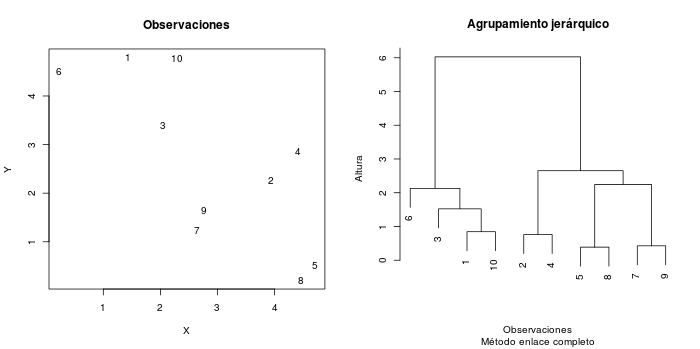
\includegraphics[width=0.8\textwidth]{agrupamiento_jerarquico}
    \caption{Ejemplo de agrupamiento jerárquico realizado sobre 10 puntos colocados de forma aleatoria en el plano, agrupados utilizando la distancia euclidiana y mediante el método de enlace completo. El panel de la izquierda muestra las observaciones, representadas cada una por un número, y el de la derecha el dendrograma obtenido.}
    \label{fig:agrupamiento_jerarquico}
\end{figure}
\section{Detectando grupos en el agrupamiento jerárquico}
\label{sec:grupos_en_agrupamiento_jerarquico}
El agrupamiento jerárquico organiza los objetos en árboles (dendrogramas) cuyas ramas son los grupos deseados. El proceso de detección de grupos a partir de esta estructura se conoce como corte de árbol, corte de ramas o podado de ramas. 
\subsection{Corte de árbol estático}
El método más sencillo de podado es conocido como corte de árbol estático, y funciona definiendo cada rama contigua debajo de una altura fija de corte, como un grupo separado. La cantidad de grupos obtenidos por éste método depende fuertemente de la altura de  corte elegida. La figura \ref{fig:corte_arbol_estatico} muestra dos alturas de corte posibles y los grupos que se obtienen a partir de cada una de ellas.
\begin{figure}[h]
    \centering
    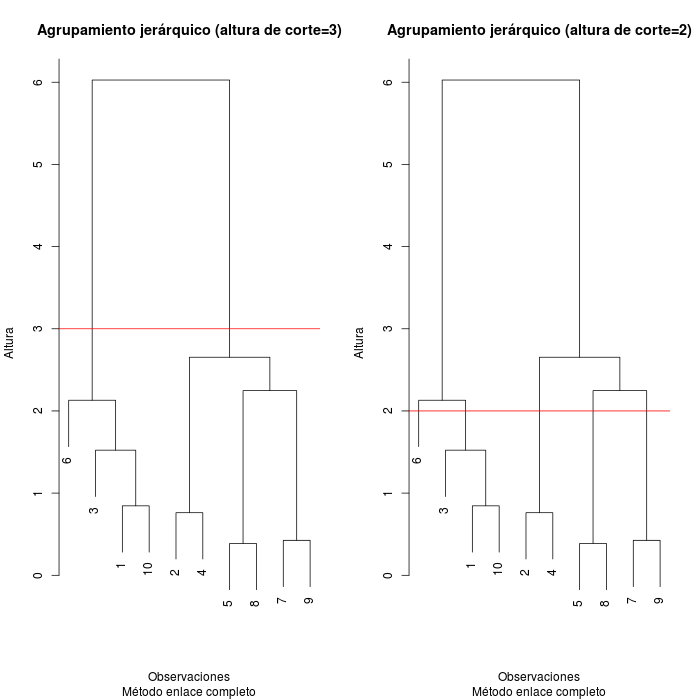
\includegraphics[width=0.8\textwidth]{corte_arbol_estatico}
    \caption{Ejemplo de corte de árbol a dos alturas diferentes. Al cortar el árbol en $h=3$, se obtienen dos grupos, el grupo $g_1$, que contiene a las observaciones $\{6, 3, 1, 10\}$ y el grupo $g_2$ que contiene a las observaciones $\{2, 4, 8, 5, 7, 9\}$, mientras que al cortarlo en $h=2$, se obtienen cuatro grupos, $g_1'$ con la observación $\{6\}$, $g_2'$ con las observaciones $\{3, 1, 10\}$, $g_3'$ con las observaciones $\{2, 4\}$ y $g_4'$ con las observaciones $\{5, 8, 7, 9\}$.}
    \label{fig:corte_arbol_estatico}
\end{figure}
Al cortar el árbol en $h=3$, se obtienen dos grupos, el grupo $g_1$, que contiene a las observaciones $\{6, 3, 1, 10\}$ y el grupo $g_2$ que contiene a las observaciones $\{2, 4, 8, 5, 7, 9\}$, mientras que al cortarlo en $h=2$, se obtienen cuatro grupos, $g_1'$ con la observación $\{6\}$, $g_2'$ con las observaciones $\{3, 1, 10\}$, $g_3'$ con las observaciones $\{2, 4\}$ y $g_4'$ con las observaciones $\{5, 8, 7, 9\}$.\\\\
Este ejemplo tan sencillo permite poner de manifiesto que el problema del agrupamiento es un problema ``mal planteado'', es decir, cualquier conjunto de puntos puede ser agrupado de maneras drásticamente distintas, sin que exista a priori un único criterio para preferir uno u otro agrupamiento. La fuente de ambigüedades a este respecto más importante, es que la forma en que los datos deberían ser agrupados, depende fuertemente de la \textit{resolución} deseada. Lo que parece una única nube de puntos puede resultar ser, al analizar los datos con mayor resolución, una partición compuesta de muchos grupos. Cada tarea deberá encontrar el nivel adecuado de resolución para obtener la cantidad ``correcta'' de grupos.\cite{Domany1999}\cite{Langfelder2008}
\subsection{Corte de árbol dinámico híbrido}
Si bien es posible detectar grupos distintos en el dendrograma a partir de una inspección visual, utilizar una técnica de corte de árbol estático de forma programática no siempre logra identificar adecuadamente los grupos, ya que al poseer grupos anidados, un solo corte a una altura prefijada no será capaz de detectarlos todos. El método de corte de árbol dinámico híbrido ataca este problema analizando la forma de las ramas del dendrograma en lugar de una altura absoluta \cite{Langfelder2008}. El mismo construye los grupos de abajo hacia arriba en dos pasos. En el primer paso, se detectan las ramas que satisfacen un criterio específico para ser grupos. Este paso de poda está basado en la información de unión del dendrograma. En el segundo paso, se miden cuán cerca de los grupos detectados en el primer paso están todos los objetos no asignados previamente. Si un objeto está suficientemente cerca de un grupo, es asignado a ese grupo. En este paso, se ignora el dendrograma y se utiliza únicamente la información de disimilaridad. Este paso puede considerarse un método modificado de particionado alrededor de medoides (modified Partitioning Around Medoids o mPAM, en inglés). Por eso el nombre de \textit{híbrido}, al tratarse de una mezcla entre agrupamiento jerárquico y no jerárquico.
Los criterios específicos para la detección de grupos se basan en los siguientes cuatro criterios de la forma de las ramas:
\begin{enumerate}
\item Un grupo debe tener una cantidad mínima de objetos.
\item Los objetos que están muy lejos del grupo son excluidos del grupo aunque pertenezcan a la misma rama del dendrograma.
\item Cada grupo debe estar separado de su entorno por una brecha o espacio vacío.
\item El núcleo de cada grupo (el conjunto de objetos con menor altura de unión en el grupo) debe estar fuertemente conectado.
\end{enumerate}
O más formalmente, dado un núcleo de un grupo, llamamos $d$ al promedio de las disimilaridades de a pares entre objetos del núcleo, es decir, a su dispersión y definimos la brecha $g$ de un grupo como la diferencia entre $d$ y la altura donde el grupo se une al resto del dendrograma y entonces, una rama se considera un grupo si:
\begin{enumerate}
\item Tiene al menos $N_0$ objetos.
\item Todas las alturas de unión son a lo sumo de $h_{max}$.
\item La brecha $g$ del grupo es mayor que un $g_{min}$.
\item La dispersión $d$ del núcleo es a lo sumo $d_{max}$.
\end{enumerate}
Los parámetros $N_0$, $h_{max}$, $g_{min}$ y $d_{max}$ son parámetros ajustables del método.
\begin{figure}[h]
    \centering
    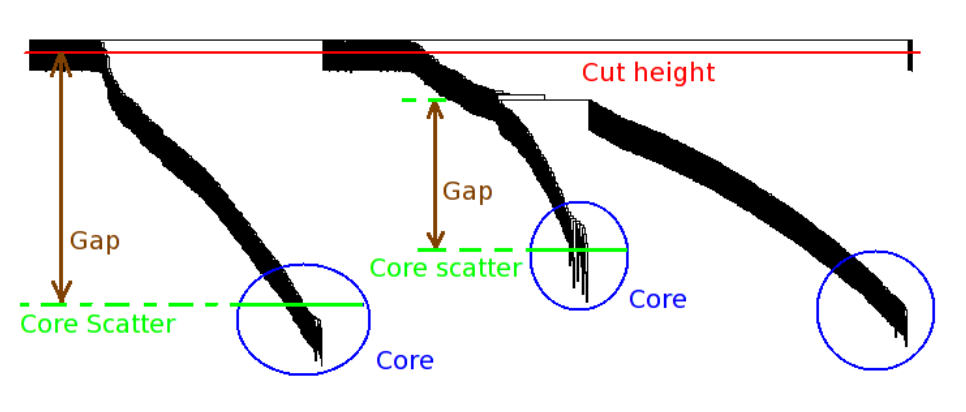
\includegraphics[width=0.8\textwidth]{cut_tree_dynamic_ejemplo}
    \caption{Dendrograma simulado con tres ramas con alturas de unión diferentes. Se observan la altura de corte (cut height), la dispersión del núcleo (core scatter), la brecha (gap) y el núcleo (core). (Fuente: Langfelder y Horvath \cite{Langfelder2008}).}
    \label{fig:cut_tree_dynamic_ejemplo}
\end{figure}
La figura \ref{fig:cut_tree_dynamic_ejemplo} muestra un ejemplo de los parámetros utilizados para definir los grupos en el paso 1.\\\\
Para el paso 2, de tipo PAM, los objetos no asignados (o aquellos grupos que no cumplan tener al menos $N_0$ objetos) son asignados al grupo más cercano si la disimilaridad correspondiente es más pequeña que una disimilaridad máxima definida previamente, o si es más pequeña que el ``radio'' del grupo. El ``radio'' se define como la máxima de las disimilaridades del medoide del grupo al resto de los objetos del mismo.\\\\
Es posible controlar la sensibilidad de las divisiones de los grupos mediante el parámetro \textit{deepSplit}, que puede tomar los valores de 1 a 4. Para un $deepSplit=1$, el método producirá relativamente pocos grupos, de muchos elementos y bien definidos, mientras que para $deepSplit=4$, el método producirá más grupos pero con una dispersión mayor en el núcleo y separado por brechas más pequeñas.\\\\
Para una descripción más detallada del algoritmo, el lector interesado puede referirse a \cite{Langfelder2008}, \cite{Langfelder2007}.

%Sin embargo, por motivos de visualización, solo se pueden representar pequeños sistemas. Las redes reales son usualmente tan grandes que es necesario representarlas mediante algún mecanismo de granularidad más gruesa, es decir, descomponer a la red en módulos que representen varios nodos y arcos. Los módulos son conjuntos de módulos que tienen un alto solapamiento topológico. Este es el objetivo básico de lo que se conoce como \textit{detección de comunidades}.\\\\

\section{Similaridad y agrupamiento en redes}
Como se desarrolló en la sección \ref{sec:redes}, las redes son construcciones útiles para esquematizar la organización de las interacciones en distintos tipos de sistemas. En particular, a partir de estas construcciones es posible estimar nociones de distancia y similaridad entre nodos. 
\subsection{Solapamiento topológico}
Una red puede representarse con una matriz de adyacencia $A=[a_{ij}]$ que codifica que pares de nodos están conectados. Para el caso de enlaces no dirigidos, $A$ es una matriz simétrica donde cada $a_{ij}$ puede tomar un valor entre $[0, 1]$. Para una red no pesada, $0$ indica que dos nodos no están conectados, mientras que $1$ indica que si lo están. Para una red pesada, el elemento de matriz es un número real que indica la fuerza de la conexión.\\\\
A partir de la matriz de adyacencia, es posible construir una matriz de solapamiento topológico $T = [t_{ij}]$ (TOM por sus siglas en inglés) que puede utilizarse como una medida de similaridad para redes biológicas y está definida como:
\begin{equation}
t_{ij} = \begin{cases} 
      \frac{l_{ij}+a_{ij}}{min\{k_i,k_j\}+1-a_{ij}} & i\neq j \\\\
      1 & i=j 
\end{cases}
\end{equation}
donde $l_{ij} = \sum\limits_u a_{iu}a_{uj}$, $k_i = \sum\limits_u a_{iu}$ y $u$ es un índice que recorre todos los nodos de la red.\\\\
El solapamiento topológico de dos nodos refleja su similaridad en términos de los nodos en común que conectan. Básicamente, $t_{ij}$ es un indicador del acuerdo entre el conjunto de nodos vecinos a $i$ con el conjunto de nodos vecinos a $j$. Utilizando esta similaridad, se obtiene una matriz de disimilaridad $D = 1-TOM$ y con esto es posible realizar agrupamientos utilizando, entre otras, alguna de las técnicas antes mencionadas. Además de TOM, es posible definir una matriz de solapamiento topológico generalizada de orden $m$, $T[m] = [t[m]_{ij}]$ (GTOMm), tal que mida el acuerdo entre los nodos que son accesibles por $i$ y por $j$ en $m$ pasos.\cite{Horvath2007}\\\\
\subsection{Detección de comunidades en redes}
\label{sec:comunidades}
En muchos casos, el análisis de patrones de interacción entre partes de un sistema, relevadas en redes complejas permite reconocer la existencia de una organización modular entre sus componentes. Esto también ocurre en muchas redes de origen biológico \cite{Barabasi2004}. De hecho, en los últimos años, muchos trabajos han explorado el vinculo existente entre comunidades de nodos en una red que representa entidades biológicas y la hipotesis de Hartwell acerca de la existencia de ``módulos de funcionalidad biológica'' \cite{Hartwell1999} que postula la existencia de agrupamientos de componentes moleculares, y sus interacciones, capaces de llevar adelante una función biológica especifica. En este trabajo utilizaremos dos métodos de reconocimiento de comunas en redes, Infomap \cite{Rosvall2008} y CNM \cite{Clauset2004}.\\\\
El método o algoritmo Infomap hace uso de criterios de optimización basados en teorías de información, donde los módulos se definen de tal forma que la longitud media de la descripción de un proceso de paseo al azar en el grafo sea mínima, mientras que el desarrollado por Clauset, Newman y Moore que denominaremos CNM, a partir de ciertas heurísticas, busca particiones de la red optimizando directamente una función de calidad $Q$.\\\\
Ambos métodos serán utilizados en este trabajo con el fin de comparar los resultados obtenidos para las comunidades Infomap y CNM con los obtenidos para los métodos de agrupamiento usados.\cite{Berenstein2014, Rosvall2008}\\\\

\chapter{Análisis de conjunto de datos transcripcionales Wiegel}
En este capítulo analizaremos el conjunto de datos transcripcionales Wiegel \& Lohmann para la planta Arabidopsis thaliana presentados en la sección \ref{sec:wiegel}, utilizando para ello los métodos de agrupamiento k-means (sección \ref{sec:agrupamientos_no_jerarquicos}) y corte de árbol dinámico híbrido (sección \ref{sec:grupos_en_agrupamiento_jerarquico}) introducidos en el capítulo \ref{materiales_y_metodos} para obtener grupos en el espacio de expresión.\\
Una vez obtenidos los grupos en el espacio de expresión, utilizaremos los índices BHI e Interacting Densities para cuantificar el grado de coherencia entre estas estructuras y los conocimientos (entendidos como nociones de similitud) en el espacio GO.\\
Luego, analizaremos la coherencia de los resultados obtenidos en el espacio de expresión con la de resultados obtenidos en otros espacios de conocimiento, como GO (sección \ref{sec:go}), PIN  (sección \ref{sec:redes}) y KEGG (sección \ref{sec:kegg}), esperando que estos conocimientos sean diferentes pero no ortogonales, utilizando para ello el índice KTA. 

\section{Descripción del dataset}
\hl{esto esta en sec:wiegel habra que profundizar mas?}
\section{Métricas transcripcionales}
\hl{esto esta en el capitulo 3, o la idea es poner otra cosa?}
\section{Agrupamiento}

\subsection{Proceso de filtrado}
El conjunto de datos Wiegel utilizado consta de los niveles de expresión de 22810 sondas que se mapean a 20149 genes a lo largo de 11 tratamientos diferentes y con entre 4 y 9 muestreos en dos réplicas. Para poder manejar esta cantidad de información es necesario realizar un filtrado (una selección) previo de los datos que permita quedarse únicamente con aquellos genes que se expresaron o inhibieron, ya que serán estos los genes que estarán siendo regulados en función del tratamiento y por lo tanto los de interés.\\
Para ello, se aplicaron dos tipos de filtros por tratamiento, por desviación estandar y por de tipo ``$K sobre A$''. Para el primero, se calculó la desviación estandar por gen a lo largo de todo el tratamiento y se decidió tomar los genes cuya desviación estandar se encontrara en el cuantil 0.9, es decir, utilizar el 10\% de los genes con mayor desviación estandar, considerando estos como los que formaron parte de la respuesta biológica al tratamiento. La figura \ref{fig:densidad_de_desviacion_estandar} muestra la distribución de probabilidad acumulada (empírica) de la desviación estandar para los genes del tratamiento ``Cold''.\\
Una vez aplicado este filtro por desviación estandar, se aplicó un filtro de tipo ``$K sobre A$'', que toma unicamente con aquellos genes que tengan al menos $K$ datos por encima del valor $A$. En nuestro caso, decidimos utilizar como valor de $K$, la mitad de las mediciones que tuviera el tratamiento. Si el tratamiento tenía mediciones cada 0 minutos, 30 minutos, 1 hora, 3 horas, 6 horas, 12 horas y 24, es decir, 6 mediciones en total, se tomó $K = 3$. Para $A$, se decidió utilizar una medida usual de $A=4$, ya que valores de señal menores a $4$ no se distinguen del ruido \hl{paper sobre esto? cuales son las unidades de estos datos? son en escala logaritmica?}. La figura \ref{fig:densidad_para_niveles} muestra la distribución de probabilidad para los niveles de expresión para el tratamiento ``Cold''.
\begin{figure*}[t!]
    \centering
    \begin{subfigure}[t]{0.4\textwidth}
    \centering
    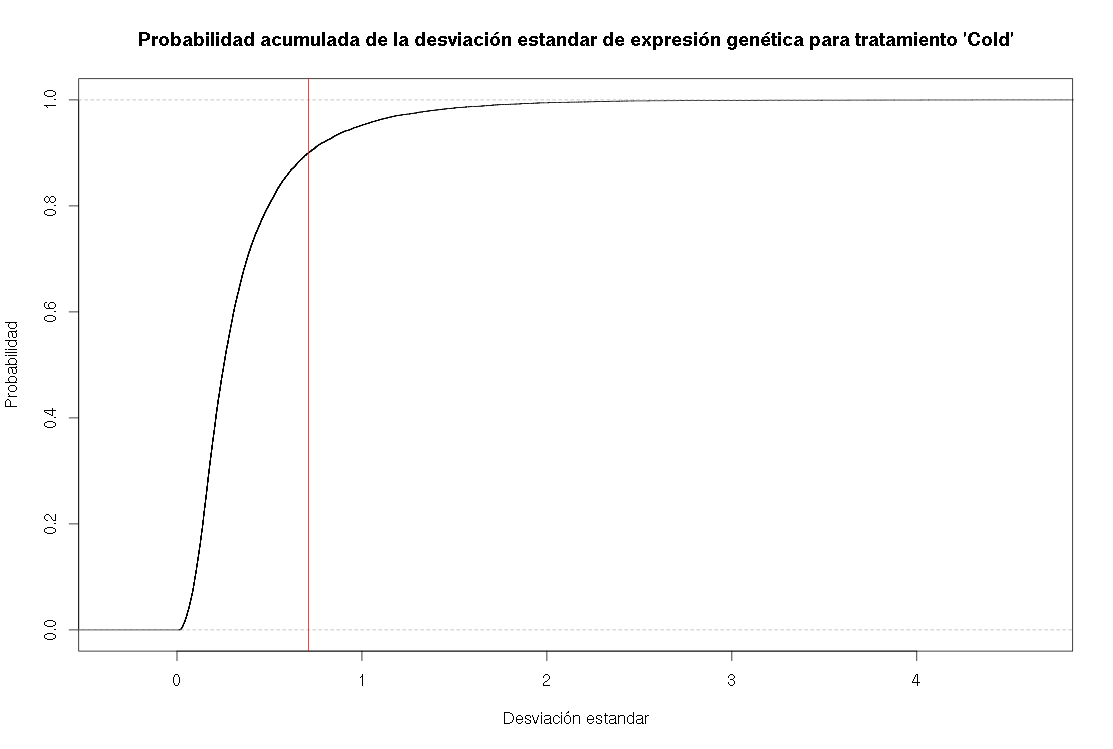
\includegraphics[width=1\textwidth]{densidad_de_desviacion_estandar}
    \caption{Distribución de probabilidad acumulada de la desviación estandar para los genes del tratamiento \textit{Cold}. Todos los genes con desviación estandar menor que la indicada por la recta vertical roja son descartados.}
    \label{fig:densidad_de_desviacion_estandar}
    \end{subfigure}
    \begin{subfigure}[t]{0.4\textwidth}
    \centering
    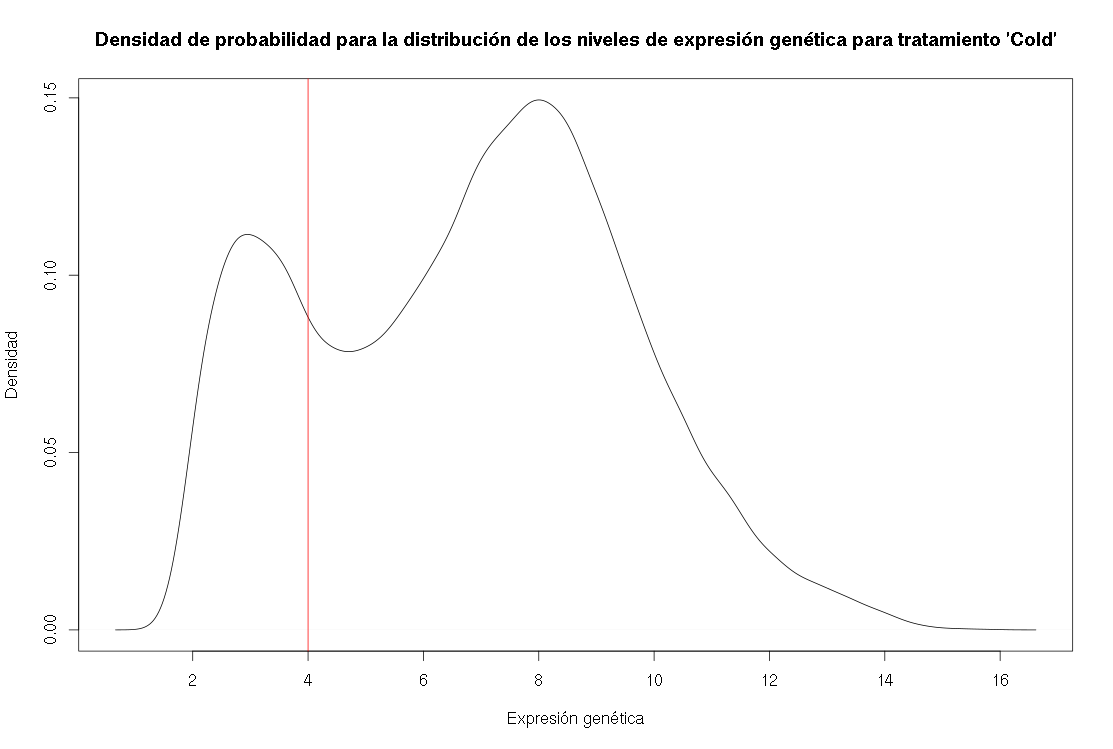
\includegraphics[width=1\textwidth]{densidad_para_niveles}
    \caption{distribución de probabilidad para los niveles de expresión para el tratamiento \textit{Cold}. La recta vertical roja muestra el valor a partir del cual se hace un corte.}
    \label{fig:densidad_para_niveles}
    \end{subfigure}
    \caption{Funciones de distribución de probabilidad para perfiles de expresión}
\end{figure*}
La tabla \ref{tabla:genes_por_tratamiento} muestra los filtros aplicados y la cantidad de genes finales por tratamiento.
Una vez aplicados los filtros y obtenido los genes de mayor variabilidad en su expresión, se estandarizaron los datos obtenidos para poner a todos los genes en igualdad de condiciones y pesarlos de la misma forma en el agrupamiento. Un procedimiento normal de estandarización de genes para que cada gen tenga media cero y varianza unitaria implica realizar la transformación:
\begin{equation}
	\tilde{x_i} = \frac{x_i-\bar{x}}{s_x}
\end{equation}
Con $x_i$ cada observación del gen $x$ a lo largo del tiempo para un determinado tratamiento. Una vez realizado el filtrado y estandarizado procedimos a agrupar los datos mediante los diferentes métodos mencionados en el capítulo 3.
\begin{table}[t]
  \centering
\begin{tabular}{| l | c | c | c |}
\hline
Tratamiento & $\sigma$ & A & Cantidad de genes \\
\hline
Control & 0.37 & 4 & 1885 \\
\hline
Frío & 0.71 & 3 & 1955 \\
\hline
Osmótico & 0.71 & 3 & 1923 \\
\hline
Sal & 0.88 & 3 & 1927 \\
\hline
Sequía & 0.54 & 4 & 1870 \\
\hline
Genotóxico & 0.46 & 3 & 1899 \\
\hline
Oxidativo & 0.41 & 3 & 1880 \\
\hline
UV-B & 0.51 & 4 & 1872 \\
\hline
Heridas & 0.41 & 4 & 1877 \\
\hline
Calor & 0.75 & 2 & 1960 \\
\hline
Calor y recuperación & 0.65 & 2 & 1944 \\
\hline                                         
\end{tabular}
\caption{Cantidad de genes y filtros utilizados por tratamiento.}
\label{tab:genes_por_tratamiento}
\end{table}
\subsection{Agrupamiento con k-means}
El método de agrupamiento k-means hace uso de la distancia euclidia para minimizar la suma de los cuadrados. Si los datos están estandarizados y centrados, es posible relacionar la distancia euclidia $d$ con el coeficiente de correlación mediante la fórmula:
\begin{equation}
	d(\vec{x}, \vec{y}) = \sqrt{2(d-1)(1-r(\vec{x}, \vec{y}))}
\end{equation}
y por lo tanto, para datos estandarizados, la distancia euclidia se comportará de forma similar a la distancia de correlación y podremos utilizar el método k-means. \hl{revisar esta frase y que quiero decir}\\
Para decidir el k a utilizar en el método, se realizó un barrido variando k entre $k=2$ y $k=30$ con pasos de 1. Al tratarse de un método heurístico, no existe garantía de convergencia al óptimo global y el resultado del mismo puede entonces depender de los grupos iniciales. Por lo tanto, para cada k, se realizaron cien agrupamientos y se midieron los índices de validación internos Calinski-Harabasz y Dunn en cada uno, definidos respectivamente como:
\begin{equation}
	CH_k = \frac{SS_B}{SS_W}\frac{n-k}{n-1}
\end{equation}
con $SS_B$ el promedio de la varianza entre grupos, $SS_W$ el promedio de la varianza intra grupos, k es el número de grupos y n el número de observaciones y:
\begin{equation}
	DI = \frac{min\delta}{\max\Delta}
\end{equation}
con $\delta$ la menor de las de distancias entre grupos y $\Delta$ la mayor de las distancias intra grupos.\\
Grupos bien definidos tendrán distancias grandes entre ellos comparados con las distancias intra grupos, por lo que a mayor $CH$ o $DI$, mejor definidos estarán los grupos.\\
Las figuras \ref{fig:barrido_k_ch} y \ref{fig:barrido_k_dunn} muestran un gráfico de caja (o boxplot en inglés), para el índice CH y Dunn respectivamente para cada uno de los k en el barrido. Un boxplot consiste en una caja con una linea horizontal que indica el segundo cuartil, es decir, la mediana del conjunto de datos, y dos lineas verticales llamadas bigotes (o whiskers en inglés) que se extiende una desde el primer cuartil hasta el valor más pequeño del conjunto (con excepción de puntos aislados) y la otra desde el tercer cuartil hasta el valor más grande. Los puntos aislados se grafican de forma separada en el gráfico.
\begin{figure*}[t!]
    \centering
    \begin{subfigure}[t]{0.45\textwidth}
    \centering
    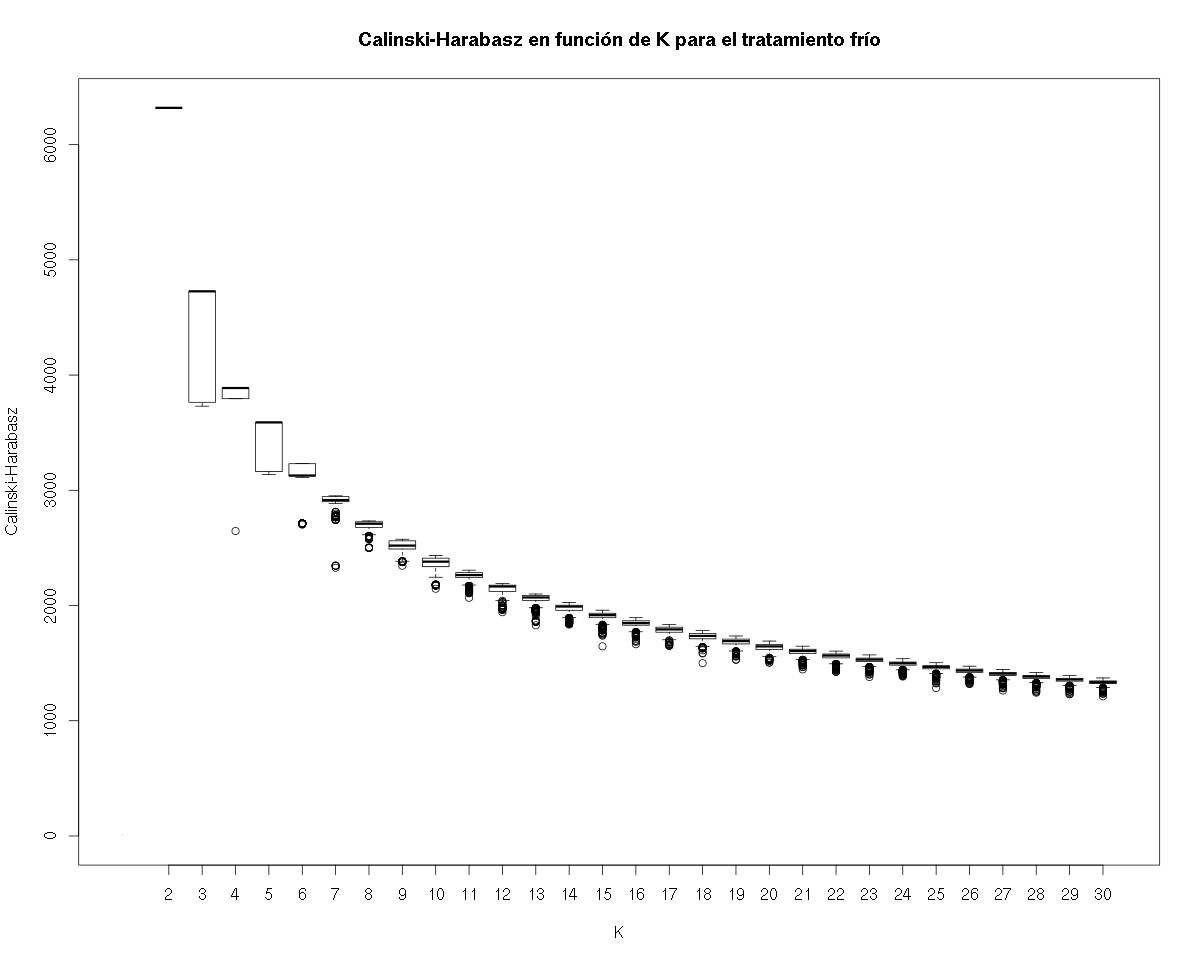
\includegraphics[width=1\textwidth]{barrido_k_ch}
    \caption{Índice CH de particiones realizadas con k-means para k entre 2 y 30.}
    \label{fig:barrido_k_ch}
    \end{subfigure}
    \begin{subfigure}[t]{0.45\textwidth}
    \centering
    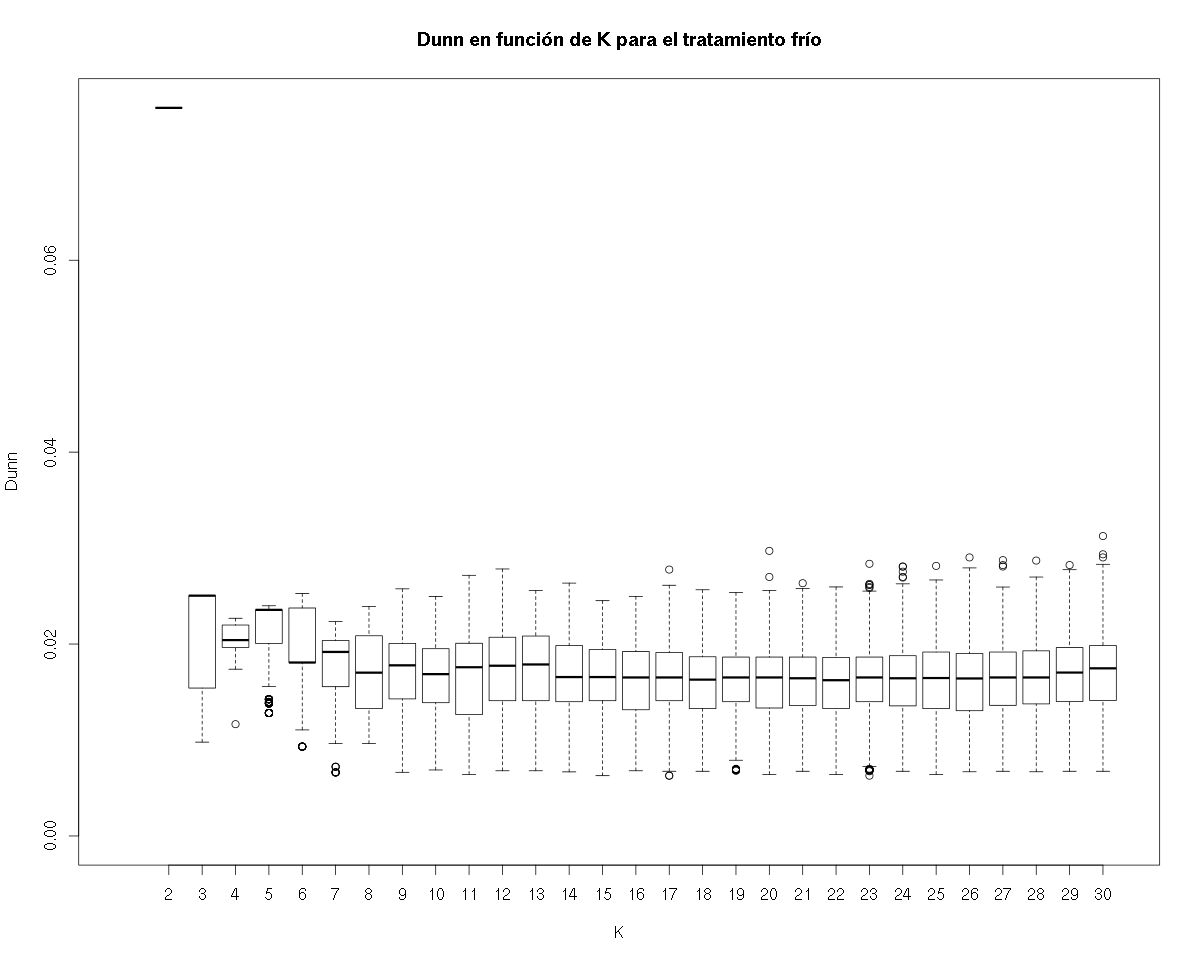
\includegraphics[width=1\textwidth]{barrido_k_dunn}
    \caption{Índice Dunn de particiones realizadas con k-means para k entre 2 y 30.}
    \label{fig:barrido_k_dunn}
    \end{subfigure}
    \caption{Índices de validación interna para particiones realizadas con k-means}
\end{figure*}
Se observa que la cantidad de grupos que maximiza estos índices es 2. Se realizó entonces un agrupamiento con $k=2$, obteniéndose los perfiles que muestra la figura \ref{fig:perfiles_k_means}, con una correlación media de $\rho=0.74$ para el primero y de  $\rho=0.79$ para el segundo, con aproximadamente el 50\% de los genes en cada grupo.
\begin{figure}[h]
    \centering
    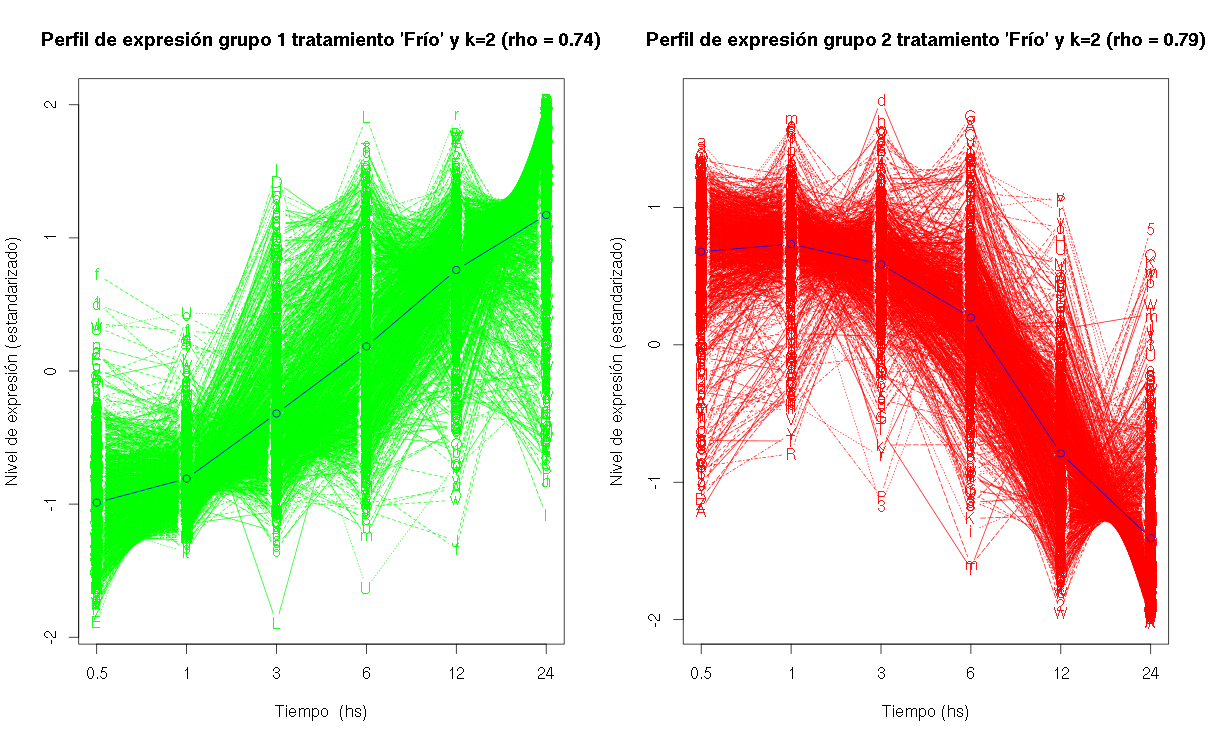
\includegraphics[width=0.8\textwidth]{perfiles_k_means}
    \caption{Perfiles de expresión génica obtenidos con el método k-means (k=2) para el tratamiento 'Frío'. En azul, el valor medio de cada grupo.}
    \label{fig:perfiles_k_means}
\end{figure}
Estas estructuras tan grandes son de difícil interpretación biológica, ya que si bien las respuestas de expresión dentro de cada grupo son similares, existe mucha heterogeneidad en las funciones biológicas de los genes que los componen. El método k-means está entonces trabajando a una escala que no permite extraer información biológica de los grupos. Será necesario entonces aumentar la granularidad mediante otros métodos de agrupamiento.
\subsection{Agrupamiento con corte de árbol dinámico}
Utilizando el método de corte de árbol dinámico se realizó para cada tratamiento 
\hl{ideas: poner aca que se probo con deepsplit 1 y deepsplit 4. Que se logra meter mucho mejor, mostrar algunos perfiles para algun tratamiento para ambos y mostrar quizas una tabla con cada tratamiento cuantos clusters y que tamanios. charlar de nuevo sobre la escala.}
\subsection{Análisis de los métodos y problemas de escala de resolución}

\section{Coherencia entre la métrica transcripcional y otros espacios de conocimiento}
\hl{idea esperamos que los conocimientos (entendidos como nociones de similitud) de los distintos espacios sean diferentes pero no ortogonales...cuantificacion...veamos que estructuras son en cierto grado coherentes}
\subsection{Interacting densities}
\hl{genex1 /genex4  VS BPa/BPb/CC}
\hl{PINinfomap / KEGGinfomap/LCI para referencia}
\subsection{KTA y zKTA}
\hl{Global}
\hl{KTA Genex por tratamiento + PIN + KEGG + LCI / GOBPa, GOBPb, GOCC}
\hl{zKTA: por tratamiento Gx/GOBPa, Gx/GOBPb, Gx/GOCC, Gx/PIN, Gx/LCI, Gx/Kegg}
\chapter{Congruencia biológica}
Esperamos que los conocimientos (entendidos como nociones de similitud) de los distintos espacios (el de expresión y el biológico) sean diferentes pero no ortogonales. Por lo tanto, una vez detectadas las estructuras en distintas resoluciones en el espacio de expresión, nos interesará cuantificar la congruencia biológica de las mismas. Para ello haremos uso de varios índices, BHI, $BHI_{IC}$, $BHI_{Resnik}$, zBHI e ID que servirán como criterios biológicos de validación externos.

\section{Índice de homogeneidad biológica}
El índice de homogeneidad biológica (o BHI por sus siglas en inglés) de una partición, introducido por Datta \cite{Datta2006} es un observable que cuantifica el grado en que una partición presenta grupos biológicamente homogéneos, reportando, para cada grupo, la máxima proporción de pares de genes agrupados que comparten una misma clase funcional de Ontología Génica. Consideremos dos genes $x$ e $y$ que pertenecen a un mismo grupo $D$ de una partición dada, con un total de $k$ grupos, y sean $C(x)$ y $C(y)$ los conjuntos de todas las clases funcionales que tienen anotados a los genes $x$ e $y$ respectivamente. Sea además la función indicadora $I(C(x)=C(y))$ que toma el valor $1$ si hay al menos una clase en donde ambos genes estén anotados, y $0$ en caso contrario. Entonces, el índice de homogeneidad biológica queda definido como:
\begin{equation}
	BHI = \frac{1}{k}\sum\limits_{j=1}^k\frac{1}{n_j(n_j-1)}\sum\limits_{x\neq y\in D_j}I(C(x)=C(y))
\end{equation}
con $n_j$ la cantidad de genes anotados en el grupo $D_j$.\\

\subsection{Modificaciones al Índice de homogeneidad biológica}
\label(subsec:control_nulo}
Presentaremos a continuación dos variantes del BHI que modificarán la función indicadora para hacer uso de la similaridad semántica y del contenido de información génico.\\
El índice de homogeneidad biológica con contenido de información ($BHI_{IC}$) para un grupo se define como:
\begin{equation}
	BHI_{IC} = \frac{1}{k}\sum\limits_{j=1}^k\frac{1}{n_j(n_j-1)}\sum\limits_{x\neq y\in D_j}I(C(x)=C(y))IC(Gx)
\end{equation}
donde el $IC(Gx)$ es el contenido de información del gen $x$, definido como el máximo de los contenidos de información de los conceptos en los que el gen $x$ se encuentra anotado.\\
Este índice permite pesar la homogeneidad biológica de un grupo la especificidad de los genes que lo componen.\\
Por otro lado, el índice de homogeneidad biológica Resnik para un grupo, $BHI_{Resnik}$ queda definido como:
\begin{equation}
	BHI_{Resnik} = \frac{1}{k}\sum\limits_{j=1}^k\frac{1}{n_j(n_j-1)}\sum\limits_{x\neq y\in D_j}I(C(x)=C(y))Sim_{rcmax}(C(x), C(y))
\end{equation}
donde $Sim_{rcmax}(C(x), C(y))$ es como fuera definida en \ref{eq:sim_rcmax}.\\
Este índice pesa la homogeneidad biológica de un grupo por la similaridad semántica de los genes que lo componen. Notar que en $BHI_{IC}$ el peso viene dado por la especificidad de cada gen individual que compone una partición, mientras que en $BHI_{Resnik}$ el peso está dado por la similaridad semántica entre pares de genes.\\
Finalmente, el índice de homogeneidad biológica estandarizado para un grupo, zBHI, se define como:
\begin{equation}
	zBHI = \frac{BHI-<BHI_r>}{s(BHI_r)}
\end{equation}
donde $<BHI_r>$ es el valor medio del conjunto de valores del BHI del grupo para un control nulo de 1000 reasignaciones de las etiquetas de la partición y $s(BHI_r)$ es la desviación estandar de la muestra para el mismo conjunto.\\
Se realizó además dos tipos de controles nulos.\\
El primero, un control nulo que llamaremos ``control nulo 1'', se realizó tomando de entre todos los tratamientos 6000 genes que pasaron los filtros. Se formaron grupos de distinto tamaño, desde grupos de 2 genes hasta grupos de \hl{500} genes tomando genes al azar de entre los 6000 con reposición. Para cada tamaño, se realizaron 1000 grupos aleatorios y se calculó su BHI. Se encontró que el valor medio de los ensambles se mantenía aproximadamente constante, mientras que existía una dependencia de la desviación estandar con el tamaño de los grupos. Se realizaron dos ajustes por funciones de ley de potencias, para tamaños entre 1 y 50 y de 51 en adelante. Las funciones halladas permiten rápidamente obtener el BHI aleatorio medio para una partición de cualquier tamaño y su desviación estandar.\\
El segundo, que llamaremos ``control nulo 2'', consistió en realizar 1000 reasignaciones aleatorias de las etiquetas de cada partición y calcular el BHI de cada grupo de la misma. Encontramos que la media de BHI calculada de esta manera coincidía con la del control nulo anterior, pero no así su desviación estandar. Concluimos que la diferencia fundamental se basa en que en el segundo caso, en la reasignación de etiquetas, se mantiene siempre la estructura de tamaños de la partición, mientras que en el primer caso, cada grupo fue tomado por separado.\\
Para caracterizar el comportamiento de cada uno de estos índices se midieron los mismos para cada tratamiento y se calculó su correlación de a pares de índices. La figura \ref{fig:correlacion_de_a_pares_bhi} muestra las distribuciones y correlaciones de a pares para estos índices en el tratamiento ``Frío''. Se encuentra que los índices modificados tienen una alta correlación entre ellos y con BHI, y por lo tanto, no aportan más información que la que se obtiene a través del índice original. Por ser el más sencillo de calcular, es el que utilizaremos como criterio de validación externa de la calidad de una partición.
\begin{figure}[h]
    \centering
    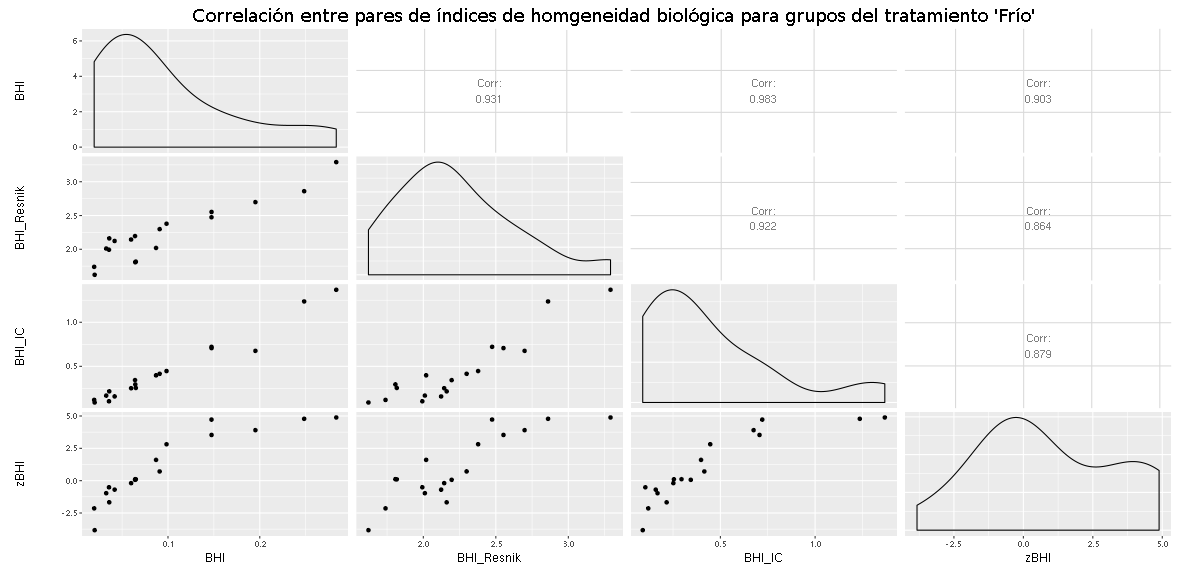
\includegraphics[width=0.8\textwidth]{correlacion_de_a_pares_bhi}
    \caption{Correlación de a pares para los distintos índices de homogeneidad biológica presentados para cada uno de los grupos del tratamiento 'Frío' obtenidos con $ds=1$. Se observa que todos los índices tienen una alta correlación entre si.}
    \label{fig:correlacion_de_a_pares_bhi}
\end{figure}

\section{Densidades de interacción}
El índice de Densidades de interacción, o ID, introducido por Dutkowski en \cite{Dutkowski2013} es un observable que cuantifica el grado en que los genes de una partición comparten anotaciones en GO y además forman parte del mismo grupo. El mismo se define para un término $j$ en una ontología GO (utilizaremos las definidas en la sección \label{sec:go}, GO BPA, GO BPB y GO CC) y una partición como:
\begin{equation}
	ID(GO_j) = \frac{NE(GO_j)}{N(GO_j)}
\end{equation}
Con $NE(GO_j)$ la cantidad de pares de genes anotados en $GO_j$ que se encuentran juntos en un mismo grupo $C_x$ y $N(GO_j)$ la cantidad de pares de genes anotados en $GO_j$.\\
Por ejemplo, para un término $GO_j$ con 20 genes anotados y una partición de 3 grupos, donde en el primer grupo hay 5 genes que están anotados en $GO_j$, en el segundo hay dos y en el tercero hay tres, obtenemos que $ID(GO_j) = \frac{\binom{5}{2}+\binom{2}{2}+\binom{3}{2}}{\binom{20}{2}}=\frac{14}{190}\approx 0.07$.\\
Además de calcular éste índice para todos los tratamientos para los métodos $ds1$ y $ds4$, utilizamos las tres redes presentadas en la sección \ref{sec:redes}, detectando comunidades en cada una mediante el método Infomap presentado en la sección \ref{sec:comunidades}.\\
Finalmente, realizamos un control nulo de tipo 2 para cada tratamiento, reordenando las etiquetas de la partición de forma aleatoria 1000 veces y calculando el $ID$ en cada caso.\\
Para cada ontología utilizada, se calculó la media de $ID$ de todos los tratamientos agrupados por cantidad de anotaciones por término, al igual que para cada una de las redes y para el control nulo. Estos valores pueden observarse en las figuras \ref{fig:interacting_densities}. Las escalas utilizadas son escalas logarítmicas. Encontramos que todas las particiones estudiadas superan los valores de $ID$ del control nulo para términos inferiores a los 2000 genes anotados, lo que implica nuevamente que los grupos poseen estructura y brindan información biológica.
\begin{figure*}[t!]
    \centering
    \begin{subfigure}[t]{0.5\textwidth}
    \centering
    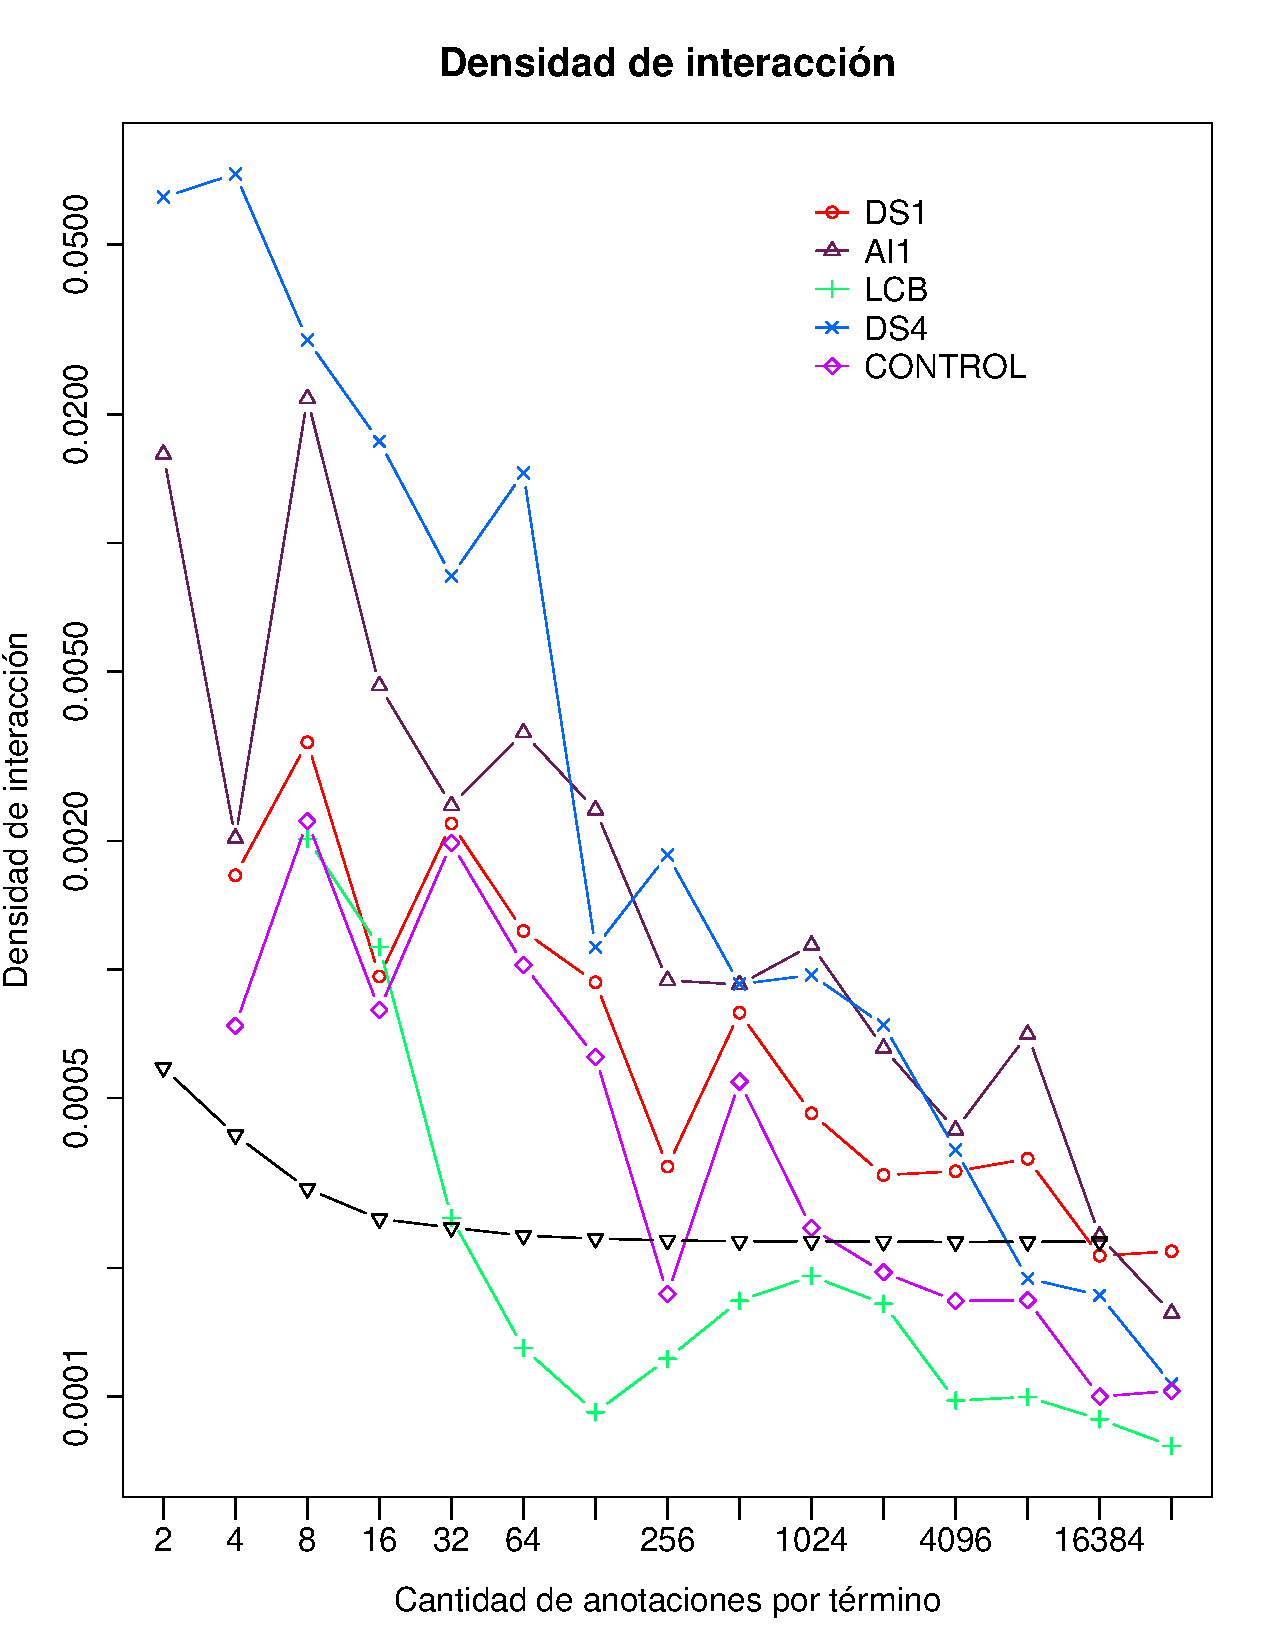
\includegraphics[width=1\textwidth]{interacting_densities_cc}
    \caption{ID para ontología CC.}
    \end{subfigure}
    \begin{subfigure}[t]{0.5\textwidth}
    \centering
    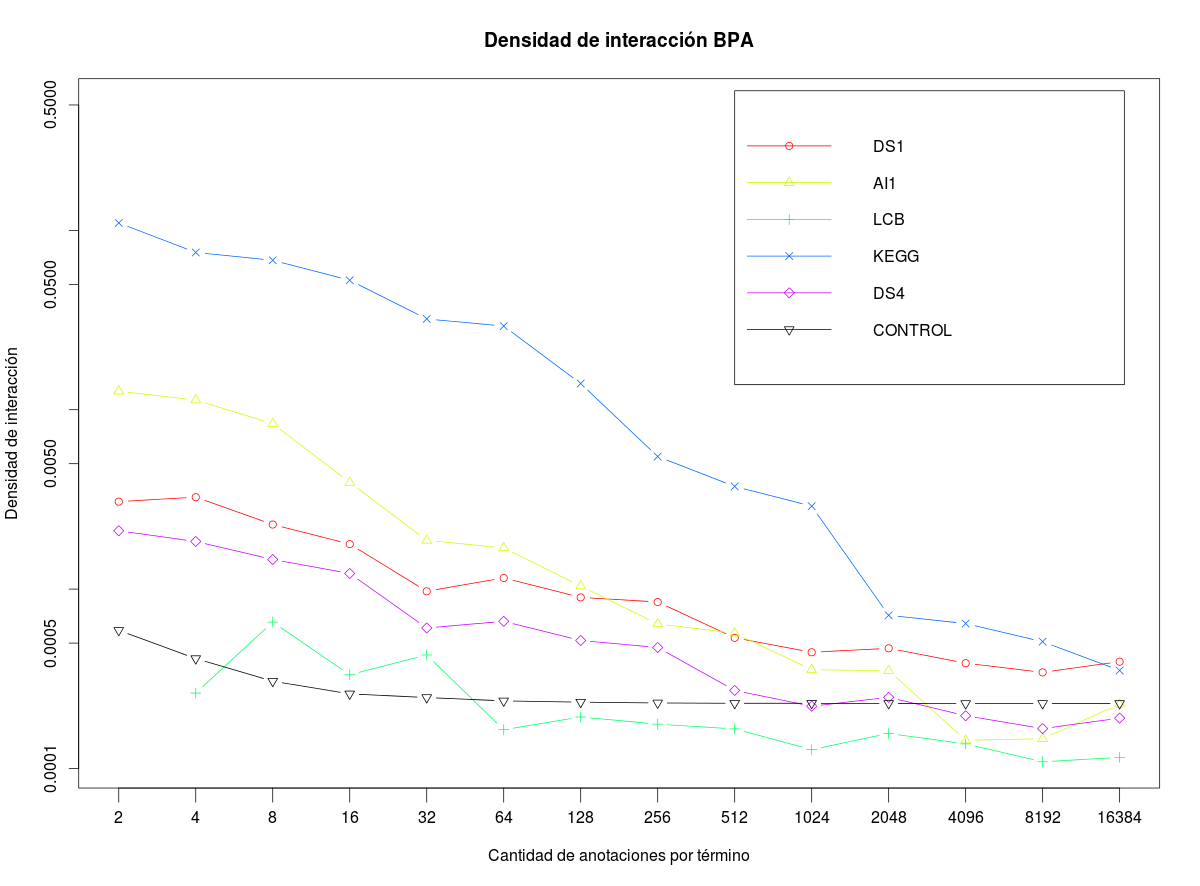
\includegraphics[width=1\textwidth]{interacting_densities_bpa}
    \caption{ID para ontología BPA.}
    \end{subfigure}
    \begin{subfigure}[t]{0.5\textwidth}
    \centering
    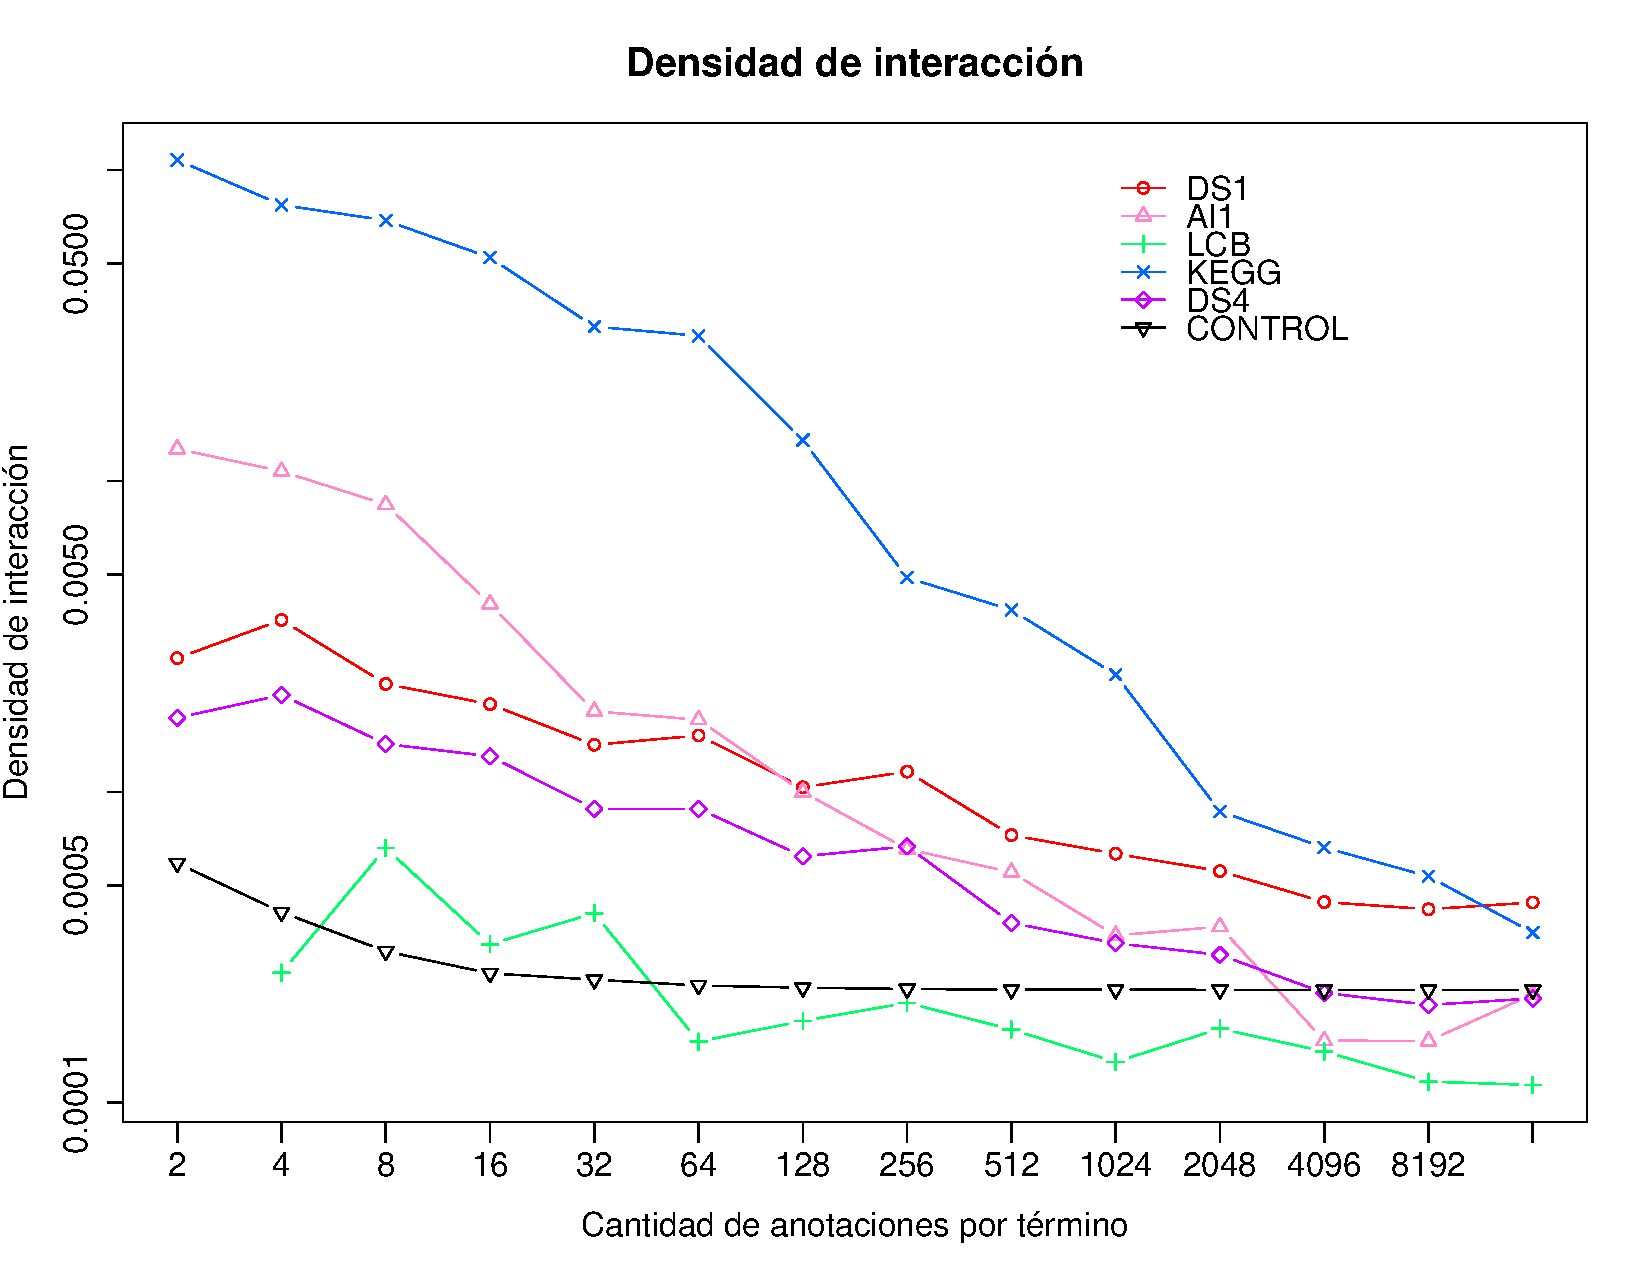
\includegraphics[width=1\textwidth]{interacting_densities_bpb}
    \caption{ID para ontología BPB.}
    \end{subfigure}    
    \caption{Índice de densidad de interacción, ID, para distintas redes de proteínas, vías metabólicas y particiones de expresión.}
    \label{interacting_densities}
\end{figure*}

Por otro lado, el control nulo se mantiene prácticamente constante para todos los términos, mientras que los otros métodos presentan variabilidad. A medida que aumenta la cantidad de genes anotados en un término, se observa una disminución del valor de $ID$ consistente con que existe una mayor cantidad de genes anotados que los disponibles en el tratamiento (por ejemplo, para el término raíz hay 10 veces más genes anotados que genes en el tratamiento). Si bien las redes de proteínas y de vías metabólicas presentan en todos los casos un $DI$ superior al de las particiones de $ds1$ y $ds4$, esto es razonable ya que estas redes fueron construidas a partir de información curada sobre interacción de proteínas, mientras que en los casos de $ds1$ y $ds4$ la interacción entre proteínas es inferida a partir de su coexpresión.

\section{Congruencia biológica de las particiones}

Los valores de BHI calculados para cada uno de los grupos del tratamiento ``frío'' en las particiones k-means (puntos rojos), $ds1$ (triángulos verdes) y $ds4$ (cuadrados azules) se presentan en las figuras \ref{fig:bhi_km_ds1_ds4_control1}, con control nulo 1 y \ref{fig:bhi_km_ds1_ds4_control2} con control nulo 2. Los grupos fueron ordenados según su masa de forma creciente.\\
Se observa que de los dos grupos de kmeans, solo uno presenta un BHI superior a una desviación estandar para el control nulo 1 y del tercer cuartil para el control nulo 2, mientras que para $ds1$, el 45\% de los grupos superan una desviación estandar para control nulo 1 y el 30\% de los grupos superan el tercer cuartil para el control nulo 2.
\begin{figure*}[t!]
    \centering
    \begin{subfigure}[t]{0.8\textwidth}
    \centering
    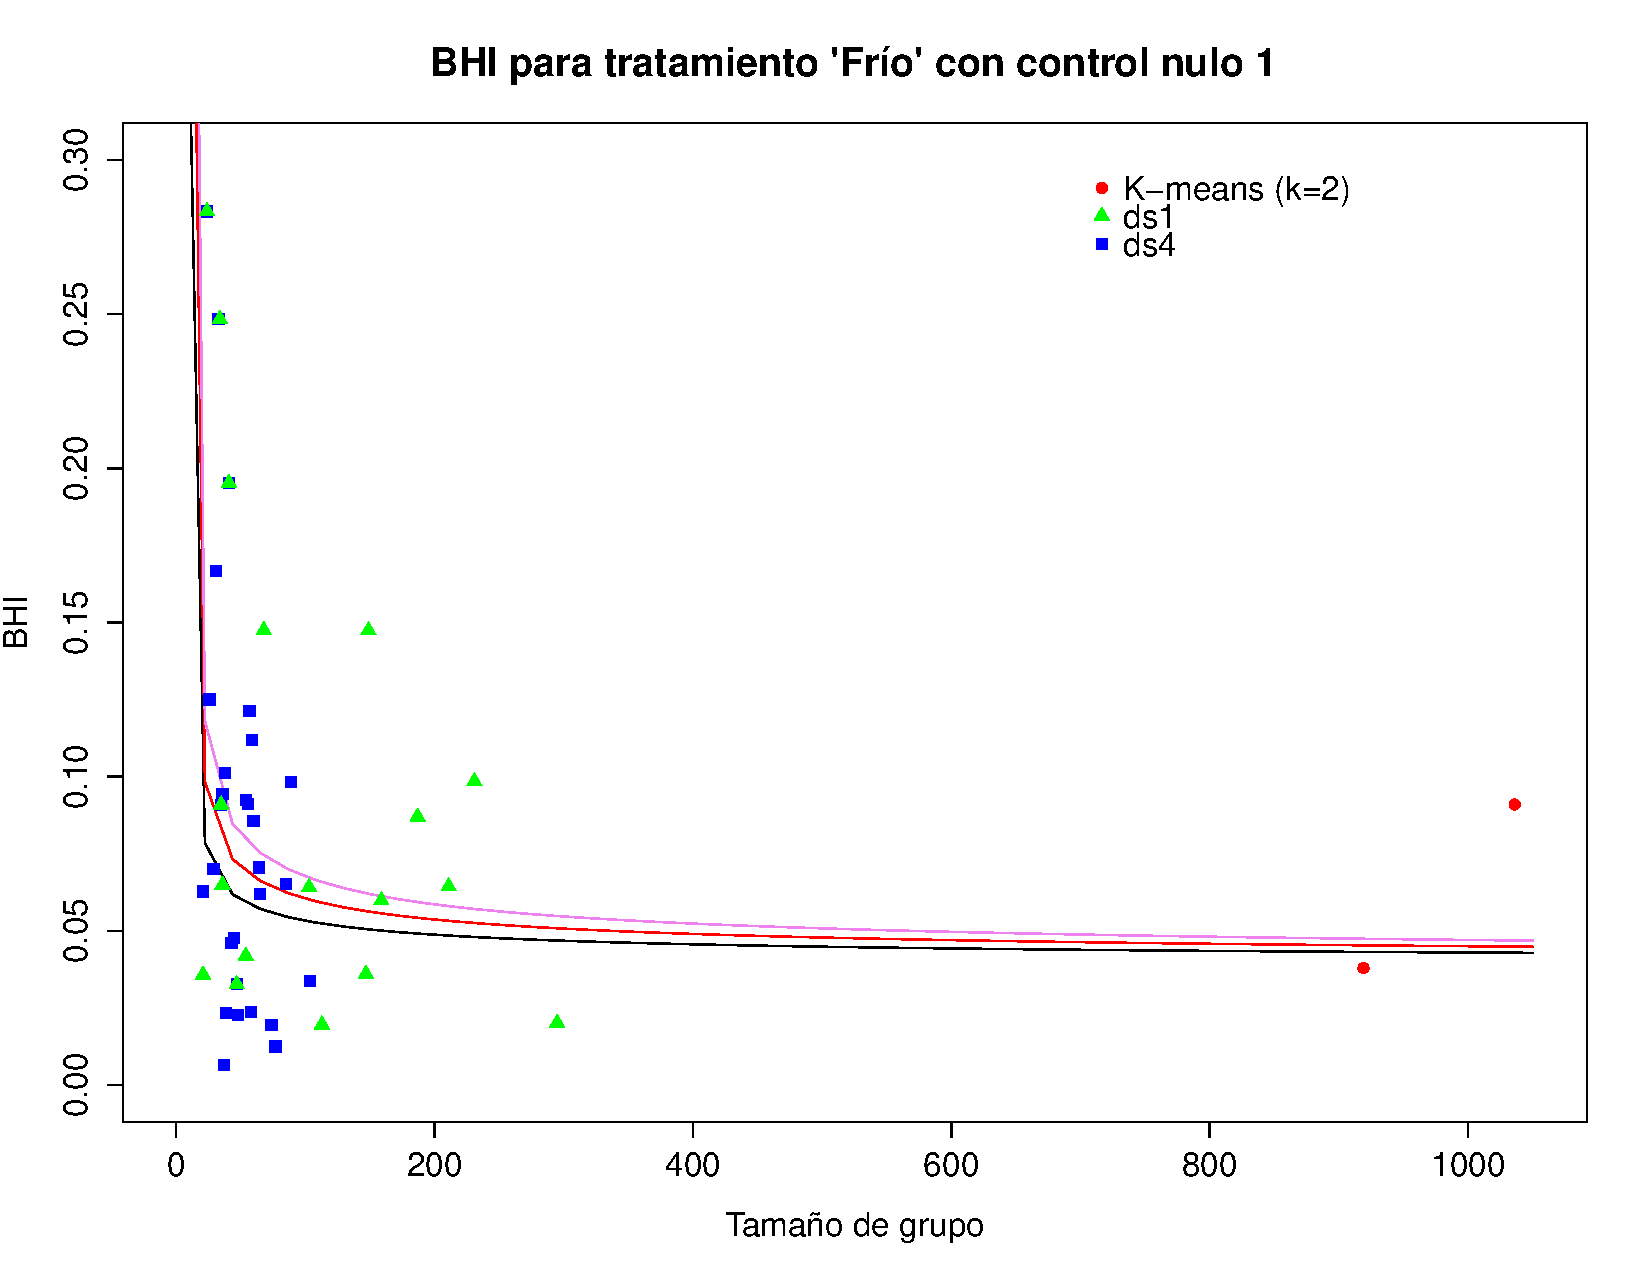
\includegraphics[width=1\textwidth]{bhi_km_ds1_ds4_control1}
    \caption{BHI para cada uno de los grupos del tratamiento 'Frío' obtenidos con kmeans, $ds1$ y $ds4$ y control nulo 1. En turquesa, el valor medio del BHI, en violeta una desviación estandar por sobre el valor medio y en negro una desviación estandar por debajo del mismo.}
    \label{fig:bhi_km_ds1_ds4_control1}
    \end{subfigure}
    \begin{subfigure}[t]{0.8\textwidth}
    \centering
    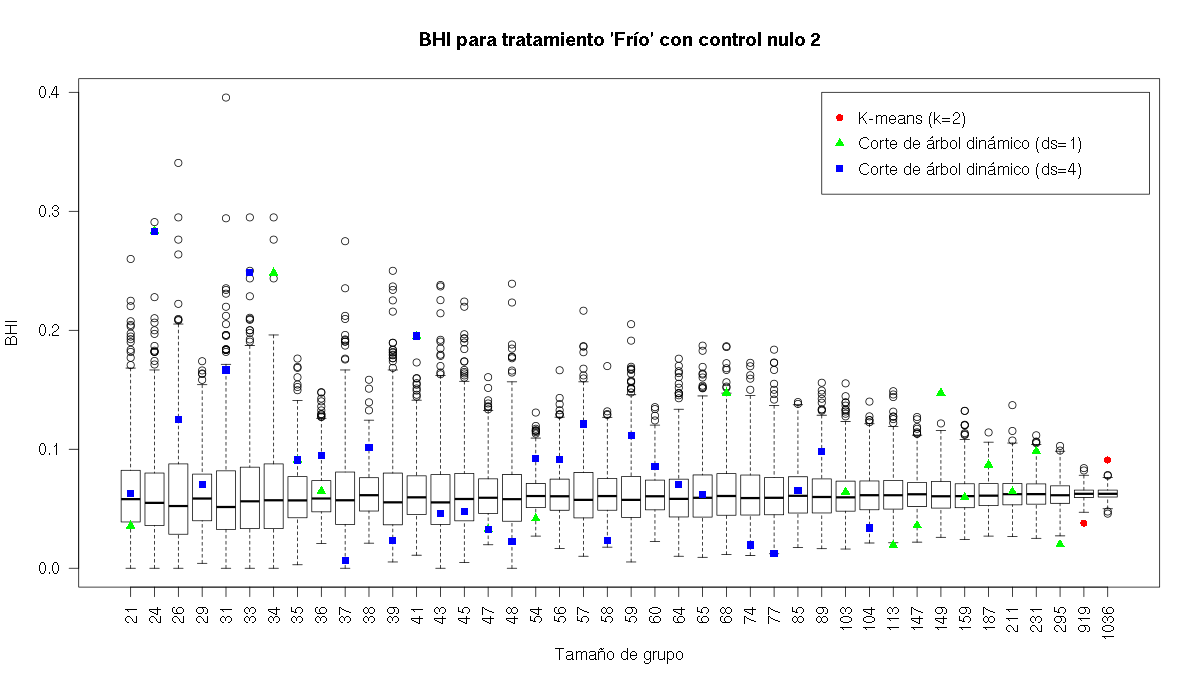
\includegraphics[width=1\textwidth]{bhi_km_ds1_ds4_control2}
    \caption{BHI para cada uno de los grupos del tratamiento 'Frío' obtenidos con kmeans, $ds1$ y $ds4$, y control nulo 2.}
    \label{fig:bhi_km_ds1_ds4_control2}
    \end{subfigure}
    \caption{Índice de Homogeneidad Biológica, BHI, para cada uno de los grupos del tratamiento 'Frío' obtenidos con kmeans, $ds1$ y $ds4$ y controles nulos.}
\end{figure*}

Finalmente, para la partición $ds4$, aproximadamente el 40\% de los grupos presenta un BHI por sobre una desviación estandar para el control nulo 1 y un 50\% presenta un BHI por sobre el tercer cuartil del control nulo 2.\\ 
Esta baja calidad en el índice BHI de las particiones se encontró de forma similar a lo largo de todos los tratamientos. Esto sugiere que si bien el aumentar la granularidad de la partición con el método corte de árbol dinámico resulta en un aumento de la consistencia biológica global de las estructuras observadas, esto no implica que las resoluciones utilizadas sean las óptimas, ya que por lo general el BHI no es superior al del control nulo.\\
A pesar de que en el análisis de estructura de los grupos obtenidos por medio de los métodos k-means, $ds1$ y $ds4$ encontramos que todos los métodos producen particiones altamente coherentes, el análisis de BHI indica que las particiones halladas no pueden ser fácilmente interpretadas a la luz del conocimiento biológico almacenado en GO.\\
En el próximo capítulo buscaremos cuantificar la coherencia entre los espacios de expresión genética y de conocimiento biológico desde una perspectiva diferente: desde la métrica en lugar de desde las agrupaciones.

\chapter{Coherencia entre la métrica transcripcional y otros espacios de conocimiento (GO)}
En los capítulos precedentes cuantificamos por medio de diversos índices la congruencia biológica de los grupos encontrados en el espacio de expresión génica. En este capítulo buscaremos cuantificar la coherencia entre los espacios de expresión génica y de conocimiento biológico desde una óptica diferente: desde la métrica en lugar de desde las agrupaciones.
\section{Alineamiento de núcleo-objetivo}
Una matriz de núcleo o matriz de Gram o matriz de kernel $K$ puede ser pensada informalmente como una matriz de similaridad de a pares entre puntos de un conjunto de datos. Para un conjunto de datos $\{x_1,...,x_m\}$ esta similaridad depende de una función $k$ llamada kernel tal que:
\begin{equation}
	K = (k(x_i, x_j))_{i,j=1}^m
\end{equation}
Una función $k(x, y)$ es un kernel si y solo si para cualquier conjunto finito de datos $C=\{x_1,...,x_m\}$ y para cualquier conjunto $\{a_1,...,a_m\} \in \mathbb{R}^m$ se tiene que:
\begin{equation}
	\sum_{i,j=1}^m a_ia_jk(x_i, x_j)\geq 0
\end{equation}
Se puede demostrar que esto implica que $K$ debe ser semidefinida positiva (SDP), es decir, $K=\sum_i \lambda _i v_i v_i'$, con $\lambda _i \geq 0$ los autovalores de la matríz $K$ y $v_i$ sus autovectores.\\
Intuitivamente, un kernel es una transformación que mapea los puntos en un espacio de alta dimensionalidad a sus posiciones relativas mediante el uso de un producto interno.\\
Existen multiplicidad de kernerls disponibles y para cada aplicación será necesario encontrar el adecuado.\\
Es de esperar que si es posible extraer información biológica del espacio de expresión genética, entonces dos puntos que son similares (en algún sentido a definir por el kernel elegido) en el espacio de expresión, también lo sean en el espacio GO (nuevamente, en algún sentido a definir por el kernel elegido). Para cada espacio habrá que definir un kernel adecuado.\\
Una forma de cuantificar la similaridad entre estos dos espacios es mediante una cantidad conocida como alineamiento núcleo-objetivo o KTA. El KTA de un kernel $k_1$ con respecto a un kernel $k_2$ del conjunto $C$ esta definido como:
\begin{equation}
	\hat{A}(S, k_1, k_2) = \frac{\langle K_1, K_2 \rangle _F}{\sqrt{\langle K_1, K_1 \rangle _F \langle K_2, K_2 \rangle _F}}
\end{equation}
Donde $\langle K_1, K_1 \rangle _F = \sum_{i,j=1}^m K1(x_i, x_j)K2(x_i, x_j)$ es el producto de interno de Frobenius entre matrices y $K_i$ son las matrices de kernels simétricas y semidefinida positivas de los espacios a comparar. Este índice tiene un rango entre $[0, 1]$.\cite{Cristianini2006}\\
Es posible extender este concepto a matrices simétricas indefinidas (no SDP) $S$ mediante diversas técnicas que consisten en transformar $S$ para obtener una $S'$ SDP. La que utilizaremos en este trabajo se conoce como \textit{corrimiento del espectro}. Si $S$ es simétrica entonces admite una descomposición en autovalores y autovectores tal que $S=U\Lambda U^T$ con $U$ una matriz ortogonal y $\Lambda$ una matriz diagonal de autovalores reales, es decir, $\Lambda = diag(\lambda _1,...,\lambda _m)$. Entonces, el corrimiento del espectro consiste en correr todo el espectro de $S$ por el mínimo necesario: 
\begin{equation}
	S_{corrida} = U(\Lambda + |\min{\lambda _{min}(S), 0}|I)U^T 
	\label{eq:matriz_corrida}
\end{equation}
Decidimos utilizar este método porque el mismo solo aumenta las autosimilaridades, sin modificar la similaridad entre dos puntos distintos, preservando la estructura de grupo al agrupar datos no necesariamente métricos.\cite{Chen22009}\\
Notar que esta medida es una medida global, ya que toma en cuenta todas las similaridades para calcular KTA.\\
\section{Espacio de expresión y GO}
Para cuantificar la coherencia métrica entre el espacio de expresión de cada tratamiento y las ontologías GOBPA, GOBPB y GOCC, utilizamos como kernel de espacio de expresión, $K_x$, la similaridad derivada de la correlación:
\begin{equation}
	K_x = (\frac{correlacion(g_i, g_j)+1}{2})_{ij}
	\label{eq:similaridad_de_correlacion}
\end{equation}
con $g_i$ y $g_j$ genes pertenecientes al tratamiento en cuestión. Se puede demostrar que una matriz de similaridad definida de esta manera es siempre SDP.\\
Para el kernel del espacio de ontologías, utilizamos la similaridad definida en la ecuación \ref{eq:sim_rcmax} y transformamos la matriz en SDP por medio de \ref{eq:matriz_corrida}. La matriz se construyó tomando en cuenta todos los genes del tratamiento. Si un gen del tratamiento no se encontraba anotado en la ontología, se lo anotaba al nodo raíz y por lo tanto su similaridad con el resto de los genes era cero. Se calculó entonces para cada tratamiento y cada ontología, el KTA y se construyó además un control nulo de tipo 2, realizando 1000 reordenamientos aleatorios de las etiquetas de la matriz $K_x$.\\
Las figuras \ref{fig:kta_global_cc}, \ref{fig:kta_global_bpa} y \ref{fig:kta_global_bpb} presentan un boxplot para cada tratamiento y cada ontología, con un punto rojo para el KTA de expresión y en negro, el KTA de control nulo. 
\begin{figure}[h!]
\centering
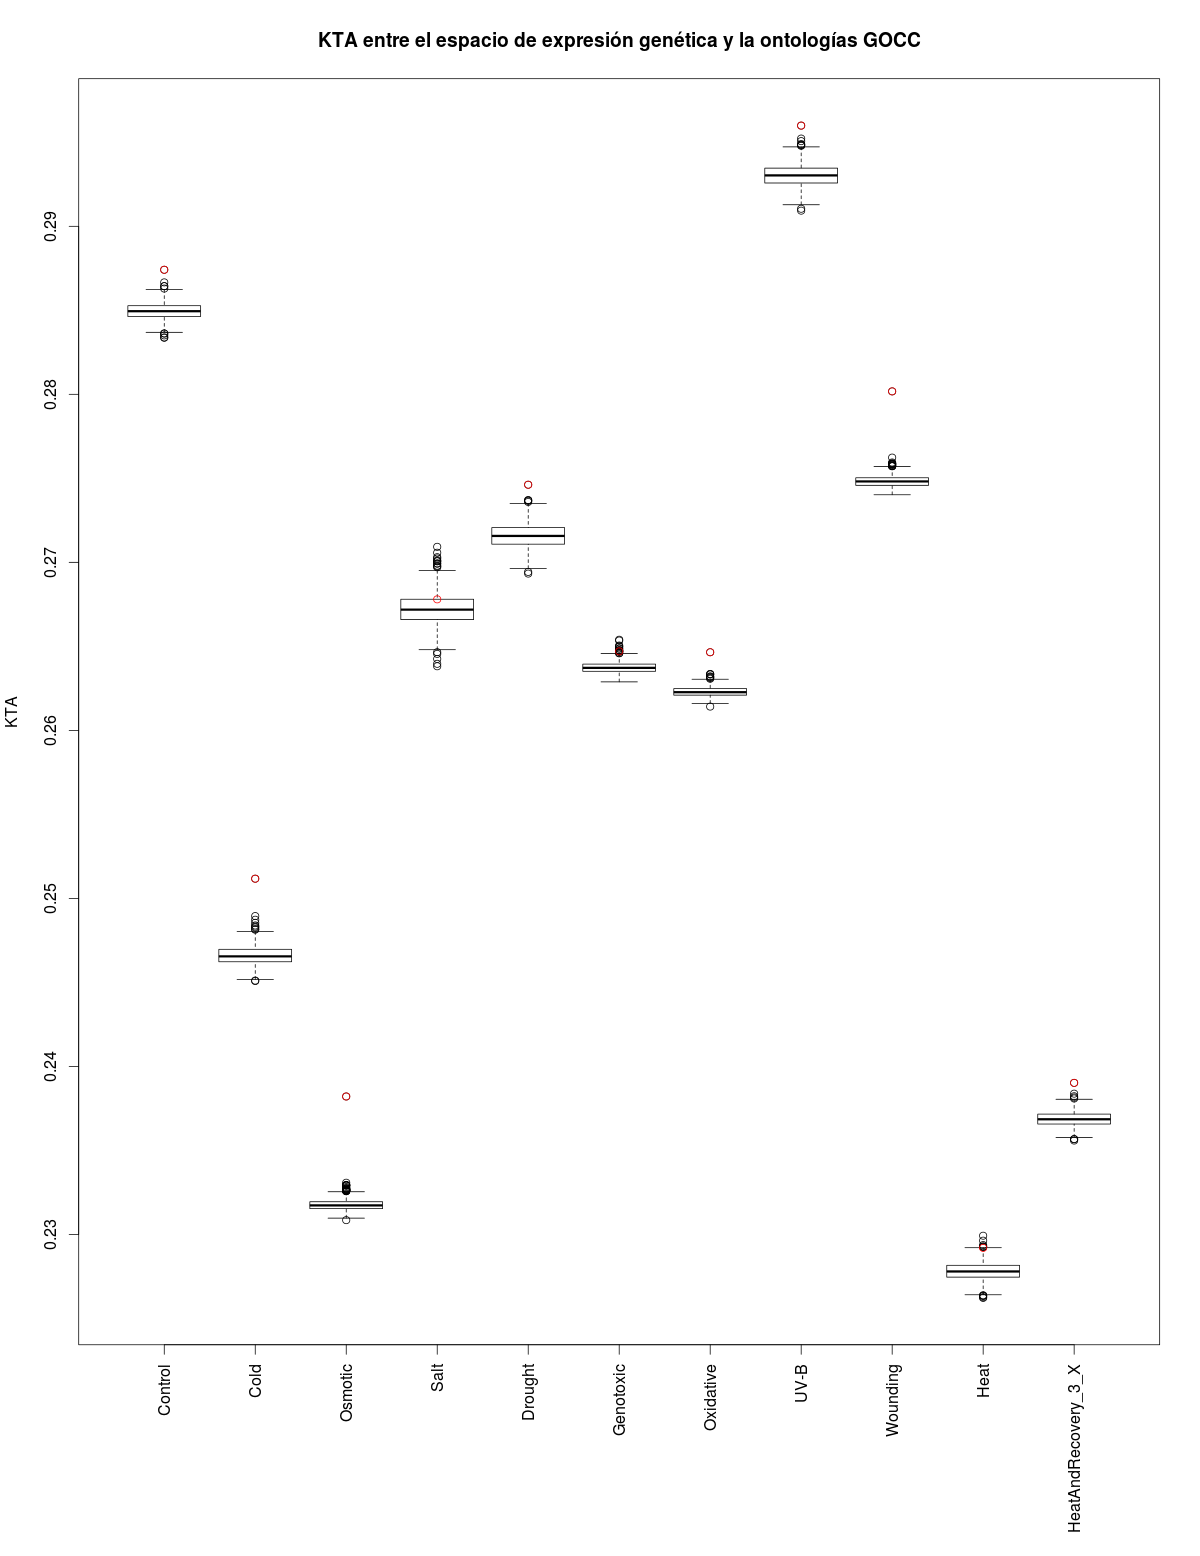
\includegraphics[height=0.4\textheight, width=0.7\textwidth]{kta_global_cc}
\caption{KTA para distintos tratamientos entre espacio de expresión y ontología CC.}
\label{fig:kta_global_cc}
\end{figure}
\begin{figure}[h!]
\centering
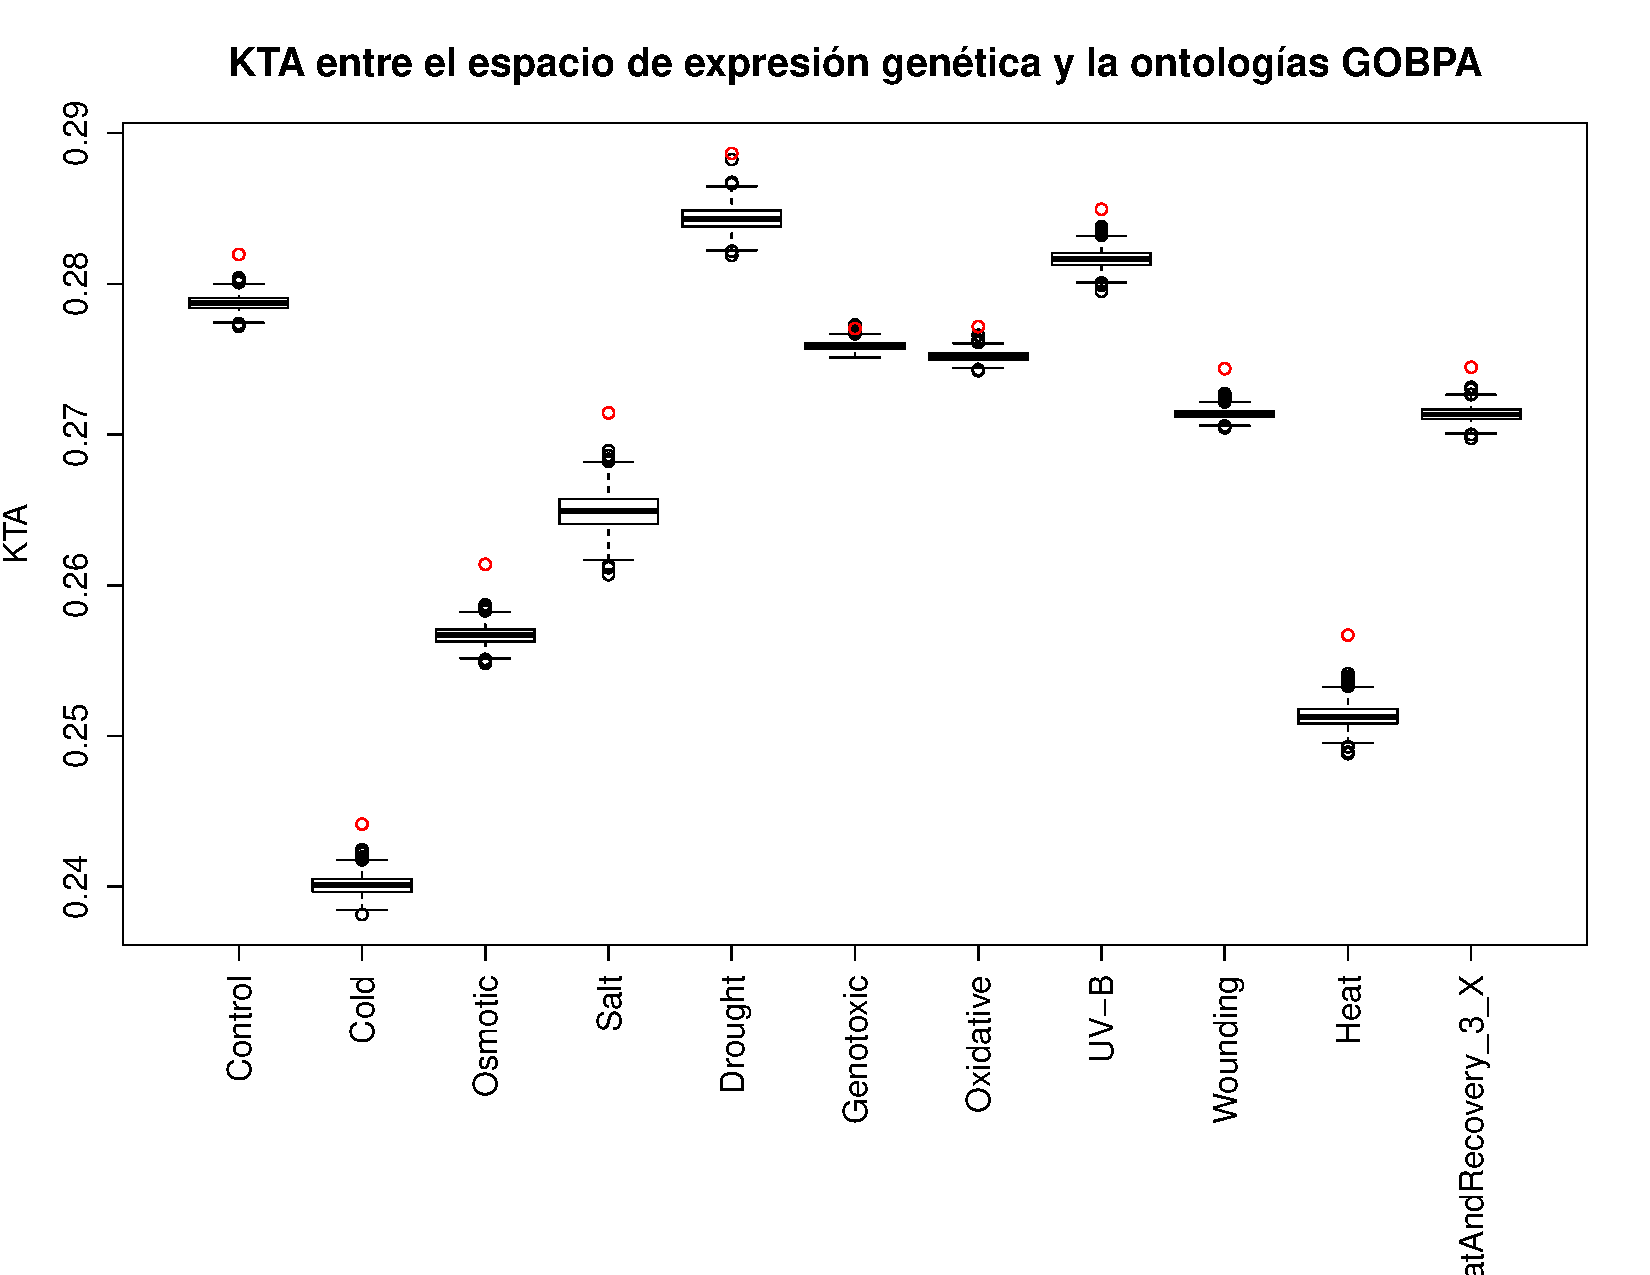
\includegraphics[height=0.4\textheight, width=0.7\textwidth]{kta_global_bpa}
\caption{KTA para distintos tratamientos entre espacio de expresión y ontología BPA.}
\label{fig:kta_global_bpa}
\end{figure}
\begin{figure}[h!]
\centering
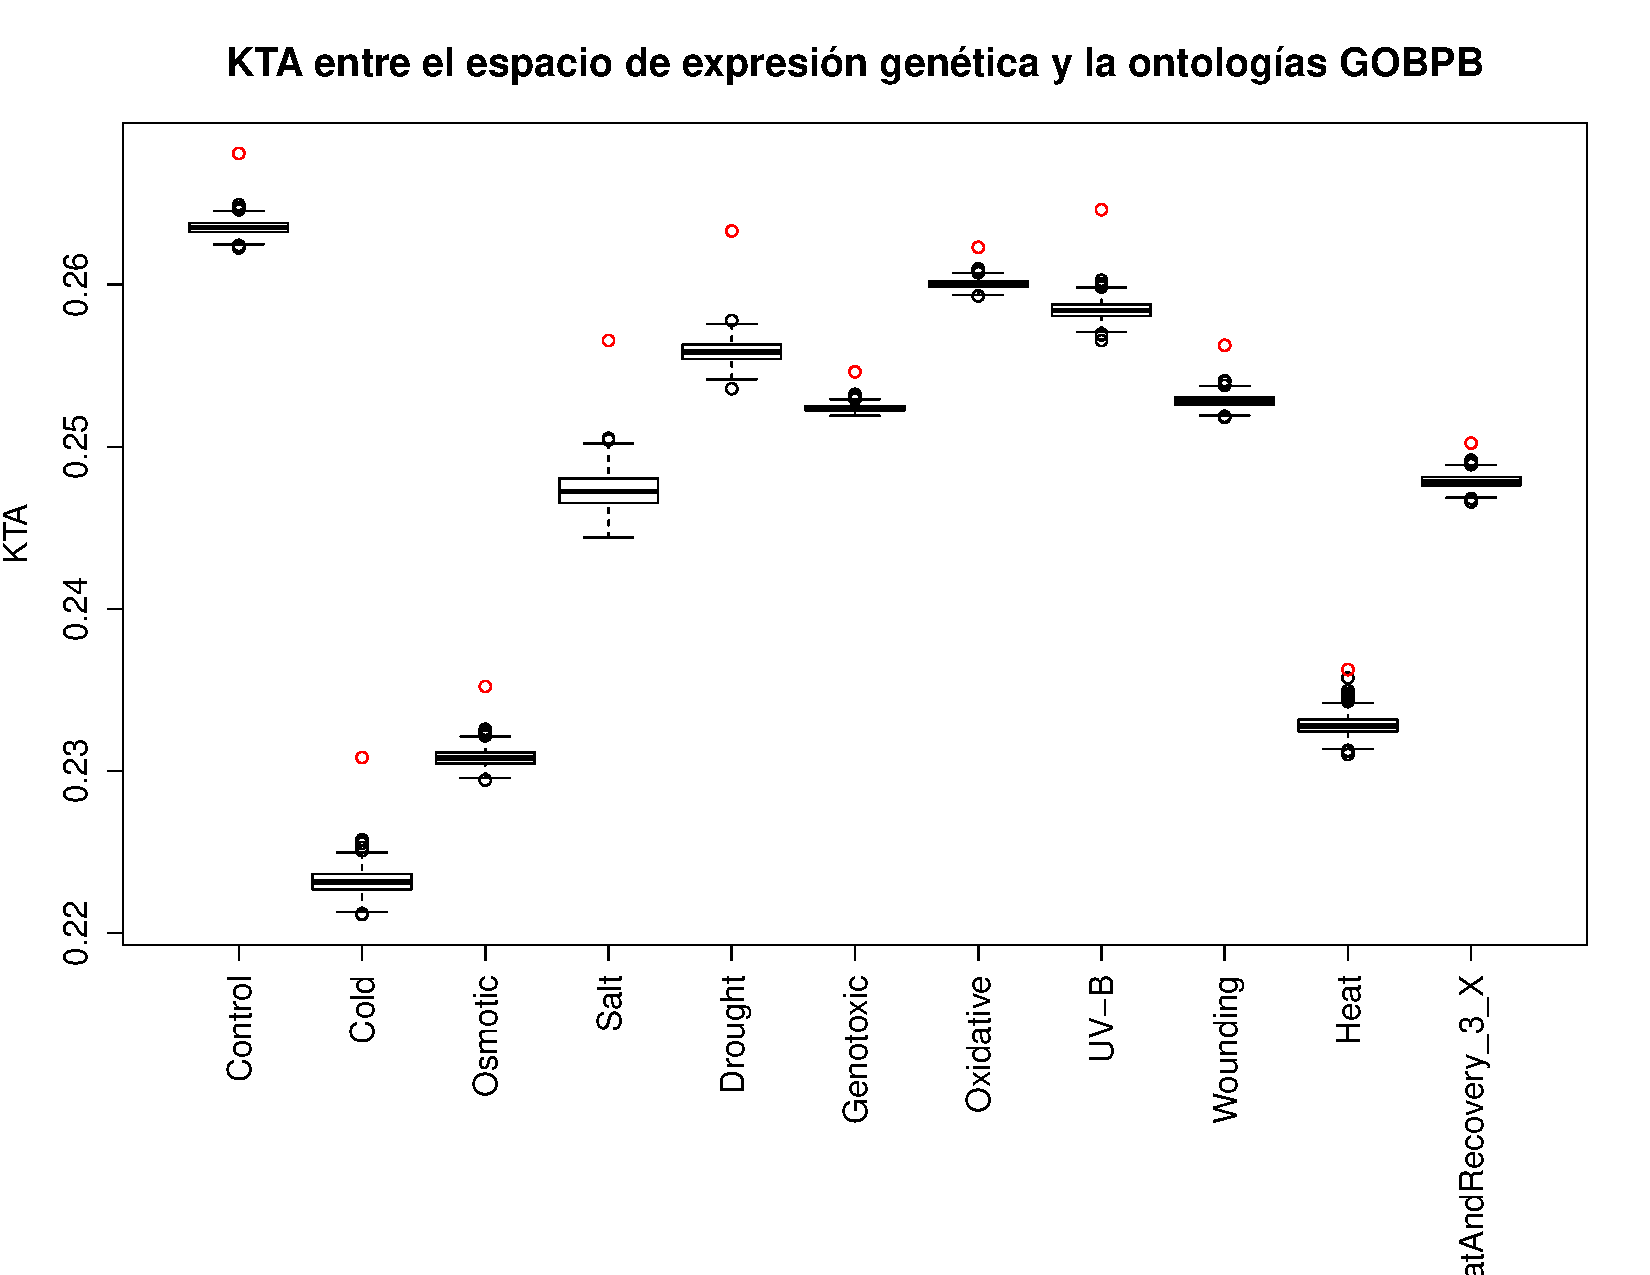
\includegraphics[height=0.4\textheight, width=0.7\textwidth]{kta_global_bpb}
\caption{KTA para distintos tratamientos entre espacio de expresión y ontología BPB.}
\label{fig:kta_global_bpb}
\end{figure}
En todos los casos encontramos que el KTA de expresión supera todos los valores del KTA de control nulo, lo que indica una coherencia entre la métrica de expresión transcripcional y la métrica del espacio GO.\\
Por otro lado, se calculó el índice KTA estandarizado definido como:
\begin{equation}
	zKTA = \frac{KTA-<KTA_r>}{s(KTA_r)}
\end{equation}
donde $<KTA_r>$ es el valor medio del conjunto de valores del KTA del grupo para un control nulo de 1000 reasignaciones de las etiquetas de la partición y $s(KTA_r)$ es la desviación estandar de la muestra para el mismo conjunto.\\
En la figura \ref{fig:zkta_global} se consignan \hl{completar esto, habia anotado esto pero pensandolo un poco no entiendo bien que poner, si no vamos a usar las redes. zKTA: por tratamiento Gx/GOBPa, Gx/GOBPb, Gx/GOCC, Gx/PIN, Gx/LCI, Gx/Kegg}\\
\hl{completar las conclusiones}
\section{Alineamiento de núcleo-objetivo local}
En la sección anterior presentamos una forma de cuantificar globalmente la coherencia entre la métrica transcripcional y el espacio GO mediante el índice KTA. Es posible redefinir este índice para obtener una medida de alineamiento de estos dos espacios pero de forma local, en las vecindades transcripcionales, para realizar un análisis de todos los genes que se expresaron o inhibieron en un tratamiento. Este índice nos será de gran utilidad en un análisis posterior para encontrar heterogeneidades en los grupos obtenidos.\hl{completar con algo mas que explique por que nos interesa hacer este analisis}.\\
Para ello, construimos tres redes de expresión, a partir de la similaridad de correlación definida en \ref{eq:similaridad_de_correlacion} entre los perfiles génicos, utilizando como topología una red pesada no dirigida con los k primeros vecinos mutuos, donde cada nodo es un gen y cada arista tiene un peso $w_{ij}$ entre $[0, 1]$ dado por la similaridad de correlación entre los dos genes $g_i$ y $g_j$ que son unidos por esa arista. Construimos redes para $k=\{5, 10, 30\}$ y estudiamos su topología.\\
\subsection{Caracterización de las redes}
Para caracterizar las redes haremos uso de dos observables topológicos, la distribución de grado y la intermediación central o betweenness centrality.\\
\subsection*{Distribución de grado}
El grado $k_i$ de un nodo de la red es la cantidad de primeros vecinos que tiene el nodo.\\
La distribución de grado $P(k)$ es entonces la probabilidad de un que nodo $i$ tomado al azar tenga grado $k$. La figura \ref{fig:distribucion_de_grado} muestran la distribución de grado para las tres redes construidas para el tratamiento 'Frío'. En rojo, la red de $k=5$, en azul, la de $k=10$ y en verde, $k=30$. \\
Se observa que el grado máximo que alcanzan estas distribuciones está relacionado directamente con el $k$ utilizado, ya que a lo sumo un nodo tendrá $k$ primeros vecinos ($k$ aristas).
\subsection*{Intermediación central o betweenness centrality}
La longitud de un camino entre dos nodos se define como la cantidad de aristas que se recorren para llegar de un nodo al otro. El camino (o caminos) más corto es aquél camino cuya longitud es la menor entre todos los caminos. La longitud de un camino más corto se conoce como distancia geodésica.\\
El betweenness centrality de un nodo $i$ es igual a la cantidad de caminos más cortos desde todos los nodos a todos los otros nodos que pasan por el nodo $i$. Es una medida de la influencia del nodo $i$ en la red, ya que un nodo con alto betweenness centrality recibirá una gran parte de la carga de la red, suponiendo que la carga se distribuye a través de los caminos más cortos.\\
Muchas redes reales presentan algunos nodos de alta conectividad, llamados hubs, por donde pasa la mayor parte de la carga de la red.\\
Las figuras \ref{fig:distribucion_de_betweenness} muestran la distribución de betweenness centrality en función del grado para las tres redes estudiadas para el tratamiento 'Frío'.\\
Se observa que las red de $k=5$ y $k=10$ presentan una gran dispersión en el betweenness de sus nodos, mientras que la red de $k=30$ tiene una dispersión menor y los nodos con mayor betweenness no son los más conectados, sino más bien los intermedios (alrededor de $k=15$).\\
\begin{figure}[h]
\centering
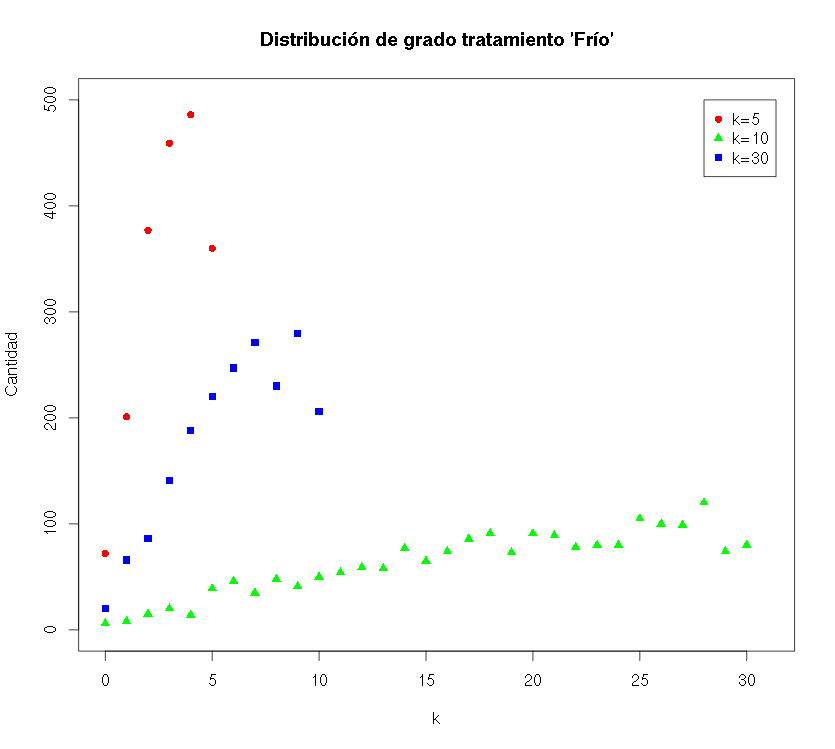
\includegraphics[width=0.8\textwidth]{distribucion_de_grado}
\caption{Distribución de grado para los nodos de las redes de k primeros vecinos mutuos, con $k=5$, $k=10$ y $k=30$ para el tratamiento 'Frío'.}
\label{fig:distribucion_de_grado}
\end{figure}
\begin{figure}[h]
\centering
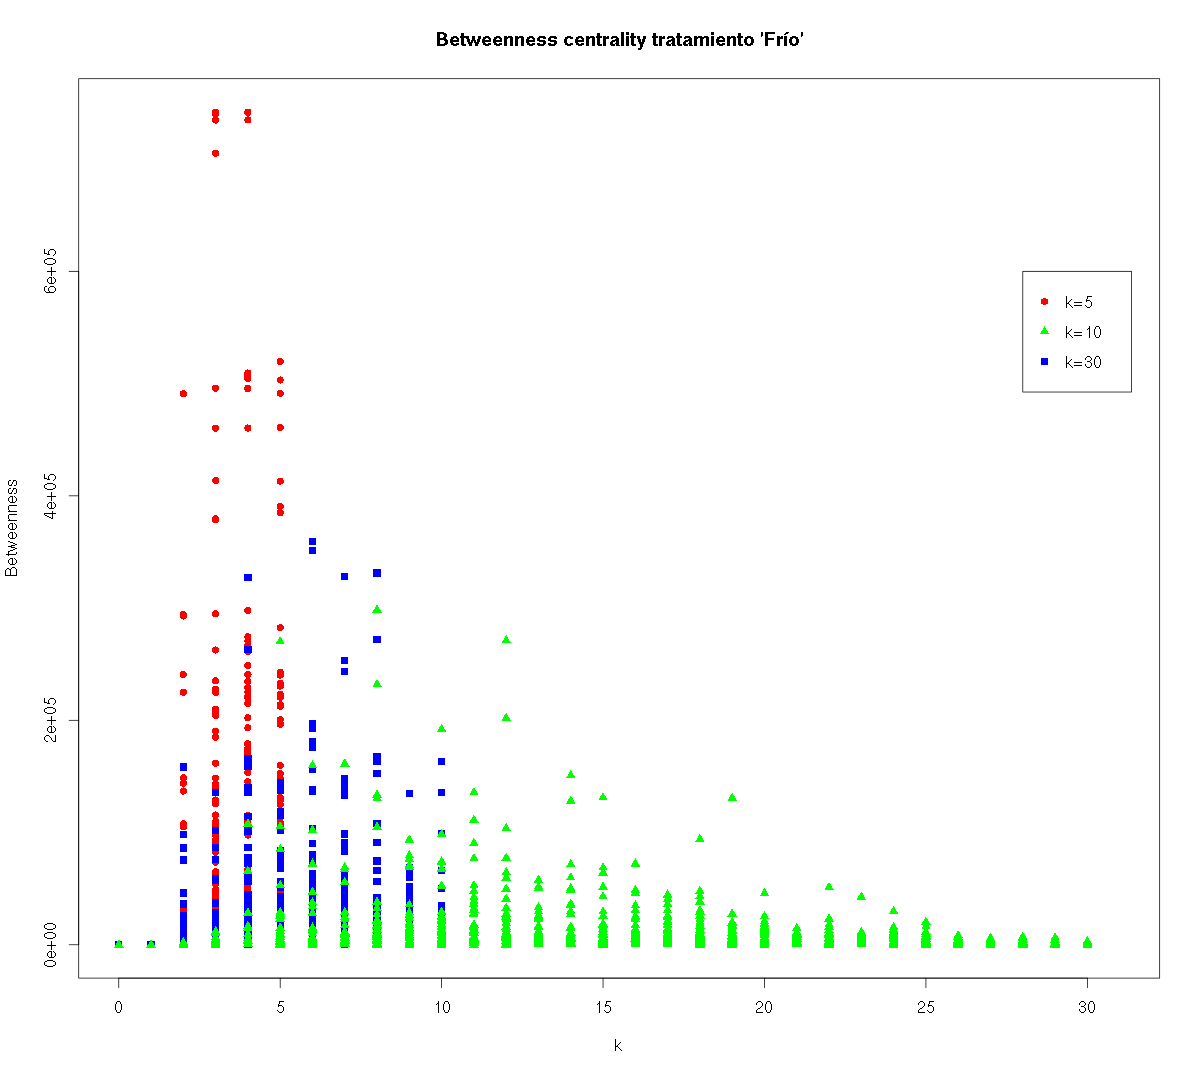
\includegraphics[width=0.8\textwidth]{distribucion_de_betweenness}
\caption{Distribución de betweenness centrality en función del grado de la red para los nodos de las redes de k primeros vecinos mutuos, con $k=5$, $k=10$ y $k=30$ para el tratamiento 'Frío'.}
\label{fig:distribucion_de_betweenness}
\end{figure}
Si bien ninguna de estas redes presenta evidencias de patrones de conectividad en su caracterización, decidimos utilizar la red de $k=30$, que llamaremos $k30$, por ser una red relativamente pequeña, en el sentido de que la cantidad de nodos y aristas (por ejemplo, 1951 nodos y 18436 aristas para el tratamiento ``Frío'') permiten realizar todos los cálculos de KTA local en un tiempo computacional razonable, pero es suficientemente grande como para poder extraer información de la misma.
\subsection{KTA local red de k=30}
Para cada arista de la red $k30$ de cada tratamiento, encontramos su vecindario local a primeros vecinos (los primeros vecinos de los nodos unidos por la arista) y construimos la matriz de similaridad de correlación reducida, consistente en la similaridad de correlación entre esos nodos y sus primeros vecinos. Generamos además la matriz de similaridad semántica reducida usando únicamente los genes anteriores, para cada una de las ontologías GOBPA, GOBPB y GOCC.\\
Aquellos genes que no estaban anotados en las ontologías, fueron anotados en la raíz de cada una respectivamente, por lo que los genes en la vecindad de un gen $i$ en el espacio de expresión no necesariamente son vecinos del mismo gen en el espacio de ontología. La figura \ref{fig:nx_vs_ny} consigna para la ontología GOBPA, la cantidad promedio de nodos vecinos anotados, $ny$, en la ontología en función de la cantidad de nodos vecinos en la red, $nx$, para todos los tratamientos. En rojo, un ajuste lineal por cuadrados mínimos. En todos los casos se observa una relación lineal entre la cantidad de vecinos en la red y de nodos en la ontología.\hl{discutir que significa esto}\\
\begin{figure}[h]
\centering
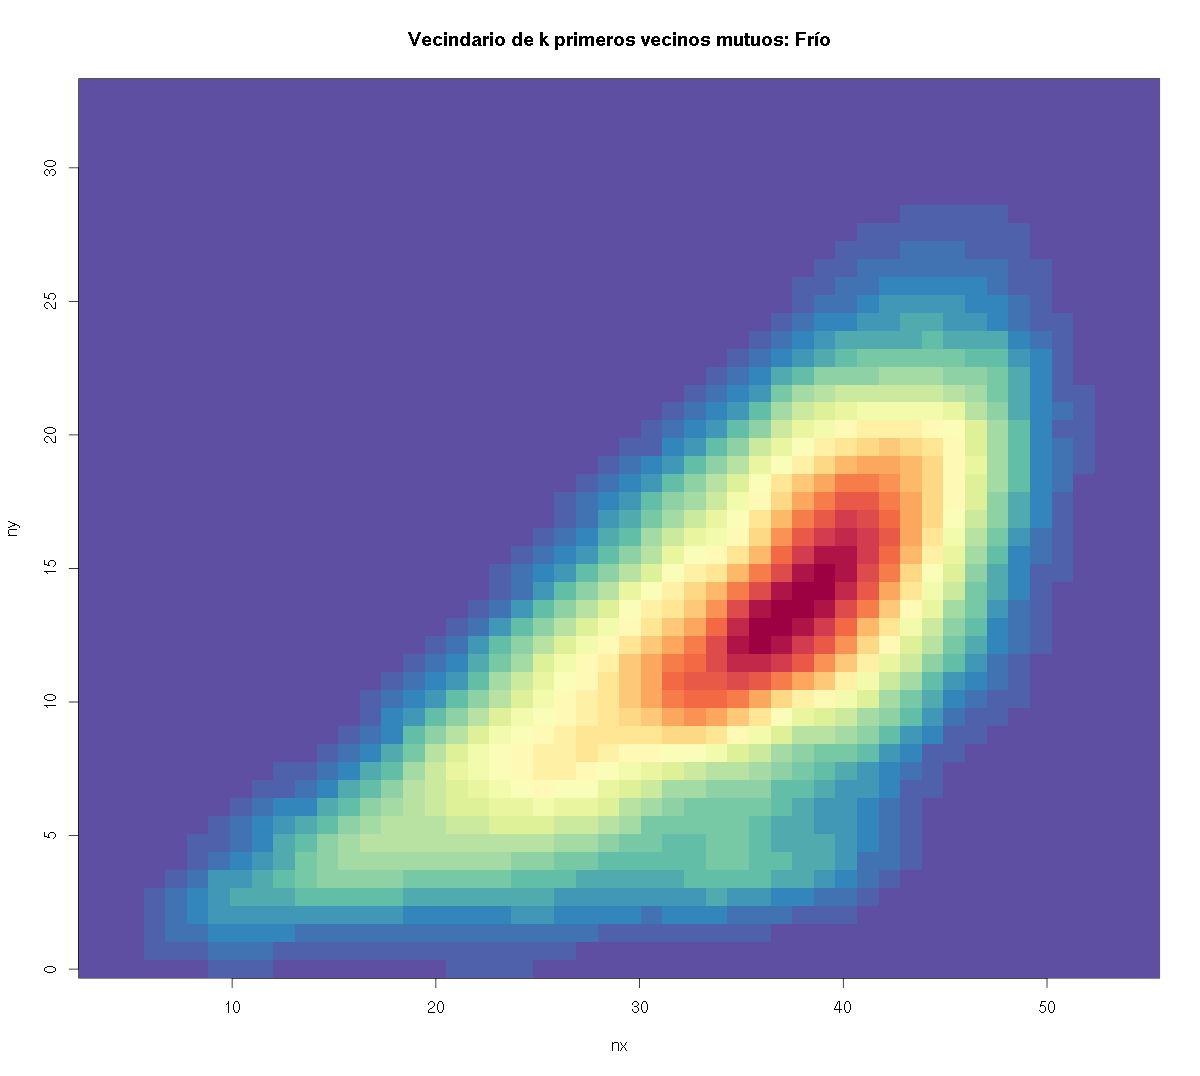
\includegraphics[width=0.8\textwidth]{nx_vs_ny}
\caption{Cantidad promedio de nodos vecinos anotados, $ny$, en la ontología en función de la cantidad de nodos vecinos en la red, $nx$, para todos los tratamientos. En rojo, un ajuste lineal por cuadrados mínimos.}
\label{fig:nx_vs_ny}
\end{figure}
Por otro lado, se calculó el valor medio de los pesos de los genes de una vecindad en el espacio de ontología, para todos los genes de la vecindad y únicamente para los anotados. La figura \ref{fig:wny_vs_wnyanotados} \hl{discutir que grafico aca y que significa lo que estoy viendo} \\
Finalmente, calculamos KTA entre la matriz reducida en el espacio de expresión y las matrices reducidas previamente transformadas en SDP de las ontologías.\\
Las figuras \ref{fig:lktaanotados_vs_wnyanotados} y \ref{fig:lktaanotados_vs_ny} muestran el KTA local solo de los genes anotados con respecto el promedio de pesos de genes anotados en una vecindad de la ontología y KTA local solo de los genes anotados y la cantidad de vecinos anotados en la ontología respectivamente. \hl{ver estos graficos e interpretar, porque no entiendo que son}






\chapter{Métrica mixta}
Como vimos en el capitulo 4 existen diferentes algoritmos de reconocimiento de agrupamientos que pueden ser utilizados para detectar, con diferente grado de granularidad, grupos de genes coexpresados.\\\\
Dichos algoritmos reportan conjuntos de genes que muestran un nivel de correlación transcripcional alto, pero pueden diferir notablemente en el grado de coherencia biológica que es posible asociar a dichas estructuras.\\\\
En este capítulo utilizaremos los resultados obtenidos en el capítulo 6 para desarrollar un procedimiento que integre la información contenida en el espacio de expresión con la información contenida en el espacio de conocimientos GO, para favorecer la búsqueda de estructuras biológicamente coherentes. La idea principal es la de montar sobre la heterogeneidad topológica embebida en la estructura de aristas de la red inferida a partir de información transcripcional, un desorden adicional modificando el valor de los pesos de dichas aristas en función de la coherencia biológica local hallada en cada caso. De esta manera, pretendemos obtener una métrica mixta que contenga información de ambos espacios.

\section{Hacia una métrica mixta}
Existen muchas formas de mezclar las métricas del espacio de expresión y del espacio GO. Una de las métricas mixtas investigadas previamente por el grupo \cite{Berenstein2010} fue la de mezcla convexa de distancias, donde se define una nueva distancia $d_{mix}$ a partir de las distancias de expresión y GO y un parámetro $\alpha$ que controla la contribución de cada métrica al algoritmo:
\begin{equation}
	d_{mix} = \sqrt{\alpha d_{x}^2 + (1-\alpha)\tilde{d}_{GO}^2}
\end{equation}
con $\tilde{d}_{GO} = \frac{\langle d_x \rangle}{\langle d_{GO} \rangle}d{_GO}$, de tal manera que coincidan los valores medios de ambas distribuciones de distancia.\\\\
Esta métrica busca el consenso a partir del parámetro global $\alpha$, que parametriza de manera continua una métrica en contraposición con la otra.\\\\
Para este trabajo, implementamos una métrica mixta que en lugar de buscar el consenso entre las métricas, penaliza las correlaciones no soportadas por las distintas ontologías e incentiva aquellas que si lo están.
\subsection{Modulación de heterogeneidades transcripcionales con información biológica}
Partiendo de la red de 30 primeros vecinos mutuos, $30kmnn$, con información transcripcional contenida en los patrones de conectividad de la red, buscamos incluir información biológica en el esquema de conexionado de la misma. Para ello, modificaremos los pesos de las aristas utilizando la información de coherencia biológica presente en KTA, tomando cada tratamiento y calculando el KTA promedio de toda la red y el KTA local de cada arista. Estas dos cantidades, el KTA promedio, que llamaremos $KTA_{fondo}$, y el KTA local de la arista entre dos nodos $i$ y $j$, que llamaremos $KTAl_{ij}$, se relacionan en una cantidad que llamaremos $stress$ y que utilizaremos como criterio para identificar si debemos penalizar o incentivar una correlación en el espacio de expresión. El $stress$ se define como:
\begin{equation}
	stress = \frac{KTA_{fondo}}{KTAl_{ij}}
	\label{eq:stress}
\end{equation}
Si $KTAl_{ij} > KTA_{fondo}$, se obtiene un $stress < 1$, mientras que si $KTAl_{ij} < KTA_{fondo}$, obtenemos que $stress > 1$. Por lo tanto, si realizamos la transformación no lineal de la similaridad de correlación:
\begin{equation}
	w_{ij} = simcor_{ij}^{stress}
	\label{eq:pesos_de_la_red}
\end{equation}
obtenemos unos nuevos pesos para la similaridad en donde aquellas relaciones que son similares en GO ($KTAl_{ij} > KTA_{fondo}$) serán incentivadas en el espacio de expresión y a la inversa, las que no son similares en GO serán penalizadas en el espacio de expresión. Los valores típicos del $stress$ oscilan entre ($0.8$ y $1.2$). Si graficamos la distribución de fuerza o \textit{strength} para los nodos de la red con los pesos modificados, definida como:
\begin{equation}
	S_i = \sum_j w_{ij}
	\label{eq:strength}
\end{equation}
obtenemos la que se observa en la figura \ref{fig:distribucion_strength_beta_1}. Esta distribución es muy similar a la distribución de grado, $P(k)$, y esto es razonable, ya que los pesos $w_{ij}$ son muy cercanos a 1 debido a la alta correlación entre vecinos de un nodo y los valores típicos de $stress$. Para poder maximizar efectivamente la heterogeneidad a nivel de pesos con información biológica, buscaremos un parámetro $\beta$ al cual elevar los pesos $w_{ij}$ tal que la distribución de \textit{strength} de la red siga una distribución de tipo ley de potencias, como propone Horvath, en \cite{Horvath2005}.\\\\
\begin{figure}[t!]
    \centering
    \begin{subfigure}[t]{0.45\textwidth}
    \centering
    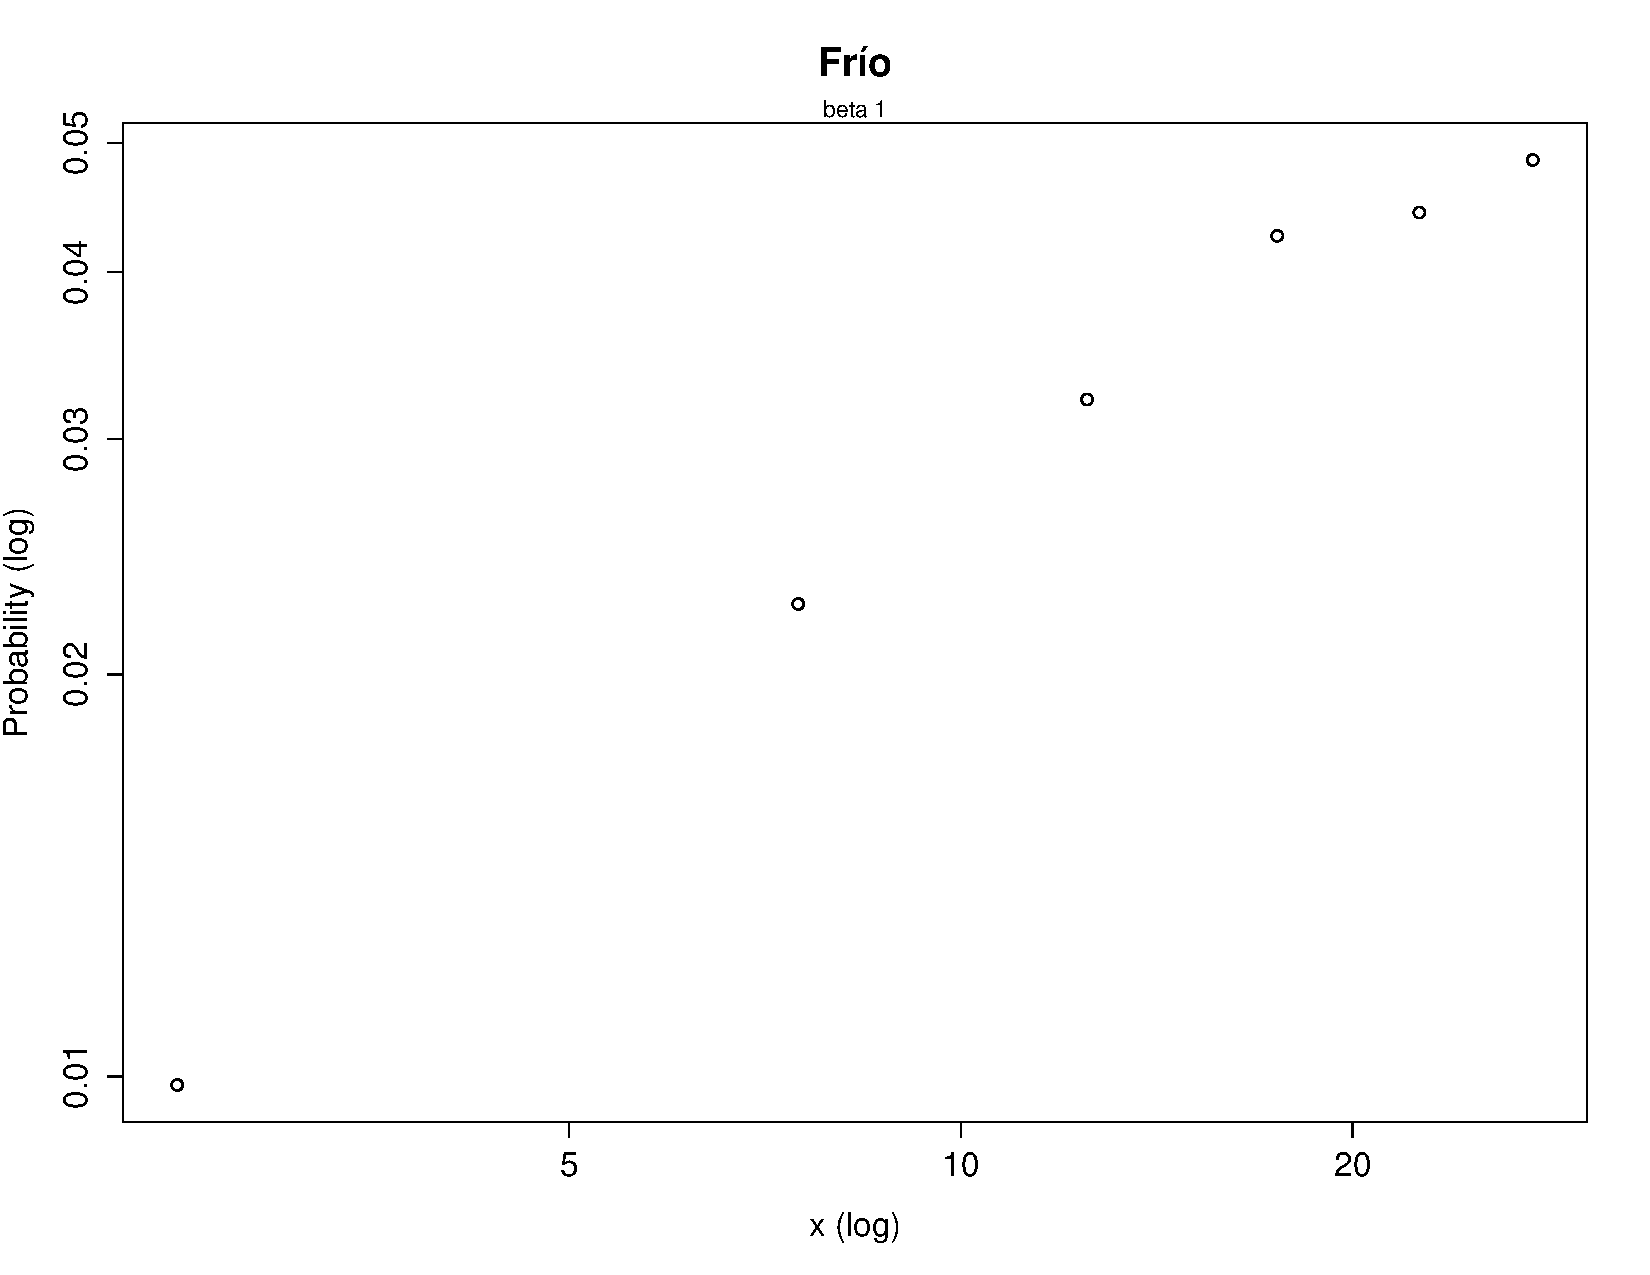
\includegraphics[width=1\textwidth]{distribucion_strength_beta_1.pdf}
    \caption{Logaritmo de la distribución de $strength$ para la red $30knmm$ con pesos $w_{ij}$ y $\beta=1$ del tratamiento 'Frío'.}
    \label{fig:distribucion_strength_beta_1}
    \end{subfigure}    
    \begin{subfigure}[t]{0.45\textwidth}
    \centering
    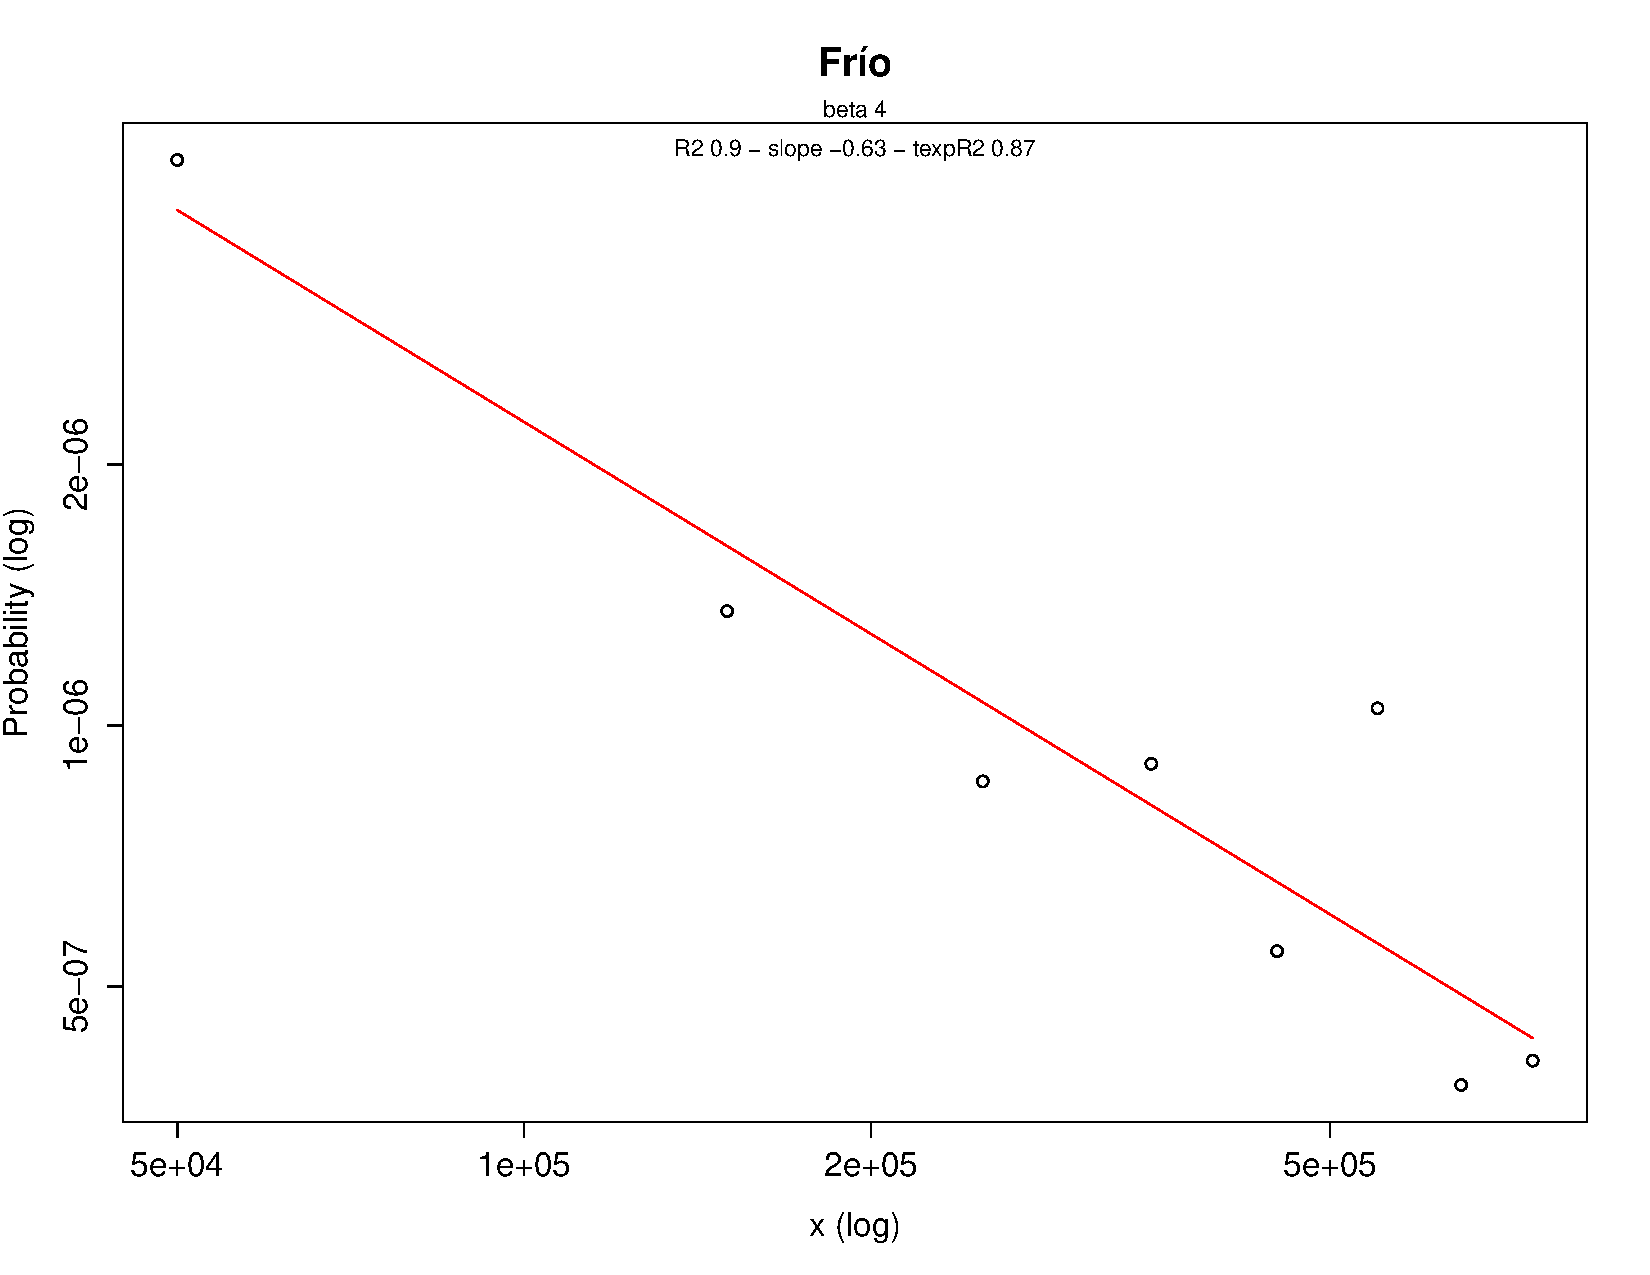
\includegraphics[width=1\textwidth]{distribucion_strength_beta_4.pdf}
    \caption{Logaritmo de la distribución de $strength$ para la red $30knmm$ con pesos $w_{ij}$ y $\beta=4$ del tratamiento 'Frío'. En rojo ajuste lineal (R cuadrado = 0.9).}
    \label{fig:distribucion_strength_beta_4}
    \end{subfigure}    
    \caption{Logaritmo de la distribución de $strength$ para la red $30knmm$ con pesos $w_{ij}$ y distintos $\beta$ del tratamiento 'Frío'.}
\end{figure}
Buscamos el parametro $\beta$ adecuado realizando un barrido para $\beta$ desde 1 hasta 4 con pasos de 1 y desde 15 hasta 65 con pasos de 5, transformando los pesos de la red como:
\begin{equation}
	w_{ij}^{'} = w_{ij}^{\beta}
	\label{eq:pesos_beta}
\end{equation}
y realizando luego un ajuste lineal para el logaritmo de la distribución de \textit{strength}. Tomamos el parámetro $\beta$ que mejor ajustaba cada tratamiento en el sentido de R cuadrado y lo utilizamos para modificar los pesos $w_{ij}$. Por ejemplo, para el tratamiento 'Frío', obtuvimos $\beta=4$ como muestra la figura \ref{fig:distribucion_strength_beta_4}.
\subsection{Heterogeneidades en escala de grupo}
La idea de nuestro enfoque es partir de los grupos detectados en el espacio transcripcional y estudiar como se comportan en términos de su coherencia biológica. Para ello pretendemos analizar heterogeneidades transcripcionales, en la escala interna al grupo, modificando la similaridad de correlación con la información obtenida mediante el índice KTA local en las redes de 30 primeros vecinos mutuos.\\\\
Para ello, tomamos cada grupo de cada tratamiento y calculamos el KTA de todo el grupo, además del KTA local de cada arista del grafo $30kmnn$ correspondiente al grupo. Con estas dos cantidades redefiniremos el $stress$ para que sea un $stress$ referido al grupo. La figura \ref{fig:distribucion_de_stress} presenta la distribución de $stress$ para el tratamiento 'Frío' en función del tamaño de grupo. Se observa que el $92\%$ de los valores de $stress$ se ubica entre $0.8$ y $1.2$, como habíamos mencionado previamente. 
\begin{center}
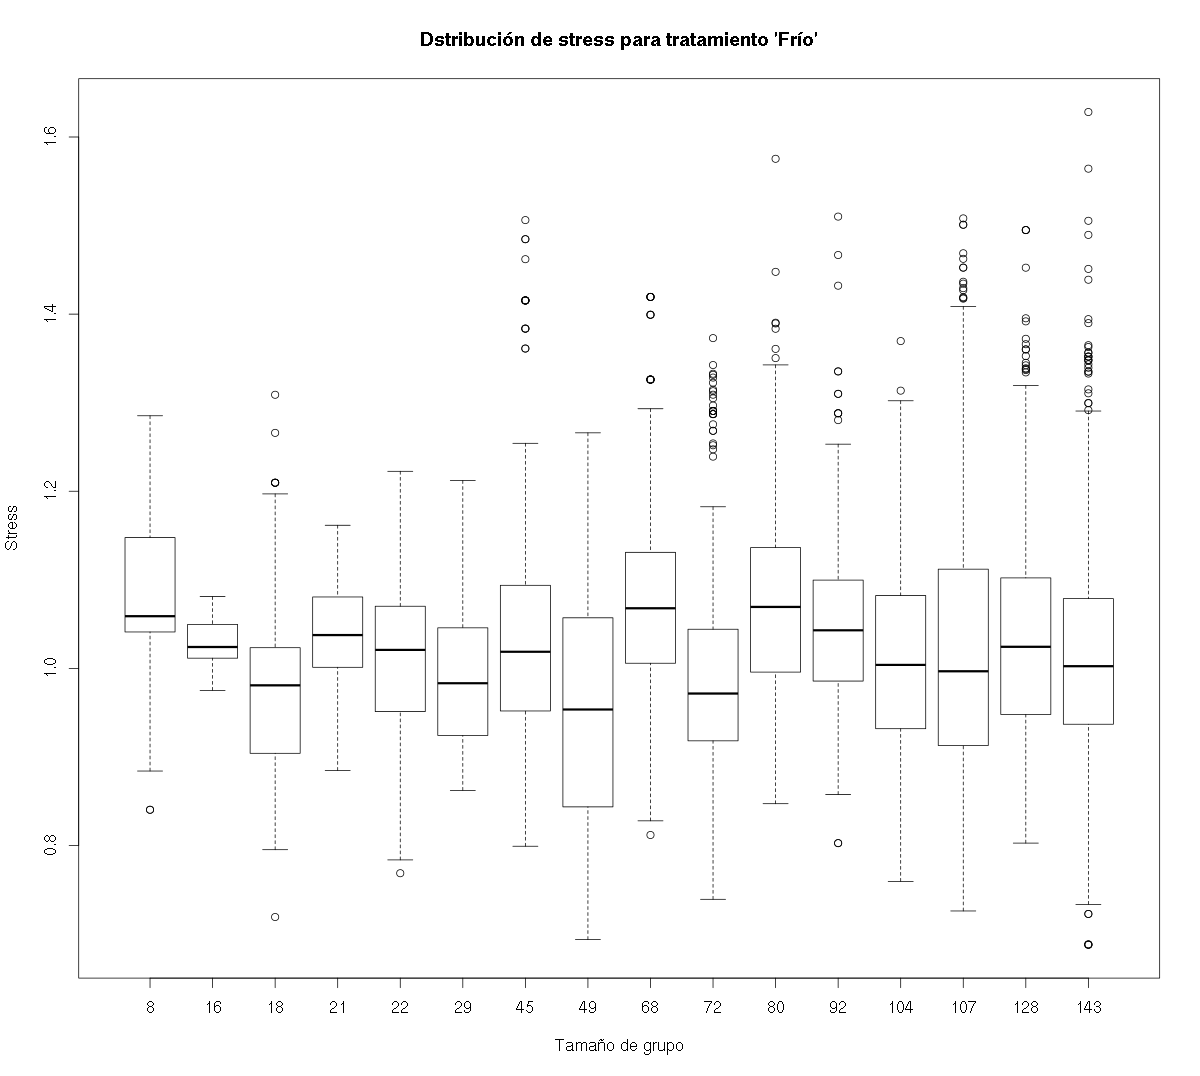
\includegraphics[width=0.8\textwidth]{distribucion_de_stress}
\captionof{figure}{Boxplot con la distribución de $stress$ para el tratamiento 'Frío' y ontología CC en función del tamaño de grupo.}
\label{fig:distribucion_de_stress}
\end{center}
Una vez obtenidos los parámetros para la métrica mixta, desarrollamos un método heurístico para poder aplicar esta nueva métrica mixta en el proceso de detección de agrupaciones de genes.

\section{Método heurístico}
El método heurístico desarrollado consiste en tomar cada grupo de una partición realizada previamente con corte de árbol dinámico e intentar encontrar subestructura dentro del mismo a partir de la métrica mixta arriba presentada de tres formas distintas.\\\\
La primera forma consiste en aplicar sobre cada grupo nuevamente un corte de árbol dinámico, utilizando la ahora métrica mixta en la confección del dendrograma, es decir: penalizando (incentivando) las conexiones más importantes, que son las que aparecen en la red de k primeros vecinos mutuas con alto (bajo) stress. A este método lo llamaremos \textit{lkta.dtc}. Por otro lado, la segunda y la tercera formas, que llamaremos \textit{lkta.infomap} y \textit{lkta.cnm}, consisten en obtener comunidades mediante infomap y cnm, respectivamente, en la red de los genes del grupo original, teniendo en cuenta los pesos modificados por la métrica mixta.\\\\
En todos los casos, una vez obtenida una partición del grupo, calculamos el índice BHI de los subgrupos obtenidos que no alcanzaron un nivel de significancia biológica suficiente y volvemos a unir aquellos subgrupos que se encuentren por debajo de una desviación estandar del control nulo 1 presentado en la sección \ref{subsec:control_nulo}. Esto lo hacemos mediante un algoritmo voraz o greedy, que en cada paso busca los dos subgrupos tales que el BHI de los dos juntos sea superior al BHI de cada uno por separado. Cuando el algoritmo no consigue unir dos subgrupos para mejorar el BHI, se detiene.\\\\ Finalmente, todos los subgrupos que todavía quedan por debajo de una desviación estandar del control nulo 1 son unidos entre sí en un único subgrupo.\\\\
Además de las 3 metodologías descriptas, utilizaremos un cuarto método, llamado \textit{insideX}, a modo de control. El mismo consiste en volver a particionar cada grupo usando corte de árbol dinámico con $deepsplit=4$, pero sin cambiar la métrica por la métrica mixta. Esto nos permitirá controlar la efectividad de la métrica mixta para encontrar mayor resolución en las particiones.\\\\
Para cuantificar el cambio en la información biológica que brinda la nueva partición, elegimos tomar el valor medio del BHI de los subgrupos, $\langle BHI \rangle$, y el valor medio del BHI de los subgrupos que superan el control nulo, $\langle BHI \rangle _{+}$. Esta ultima cantidad refleja la situación de aquellas subestructuras del grupo original que se ``beneficiaron'' desde el punto de vista del BHI, con la mayor granularidad de la nueva partición.\\\\
A modo de ejemplo, presentamos en las figuras \ref{fig:metodos_mixtos_grupo_2} y \ref{fig:metodos_mixtos_grupo_9} los resultados de esta heurística aplicada a los grupos 2 y 9 del tratamiento 'Frío'. En las mismas, la curva negra indica 1 $\sigma$, la roja 2 $\sigma$ y la verde 3 $\sigma$ de la distribución del BHI del control nulo 1. El punto lleno representa el grupo original y su BHI. En verde si su BHI supera el control nulo y en rojo si no. Los puntos vacíos en gris representan los subgrupos nuevos. En la leyenda, el primer número es $\langle BHI \rangle$ y el segundo, entre paréntesis, es $\langle BHI \rangle _{+}$.\\\\
\clearpage
\begin{sidewaysfigure}[H]
 \centering
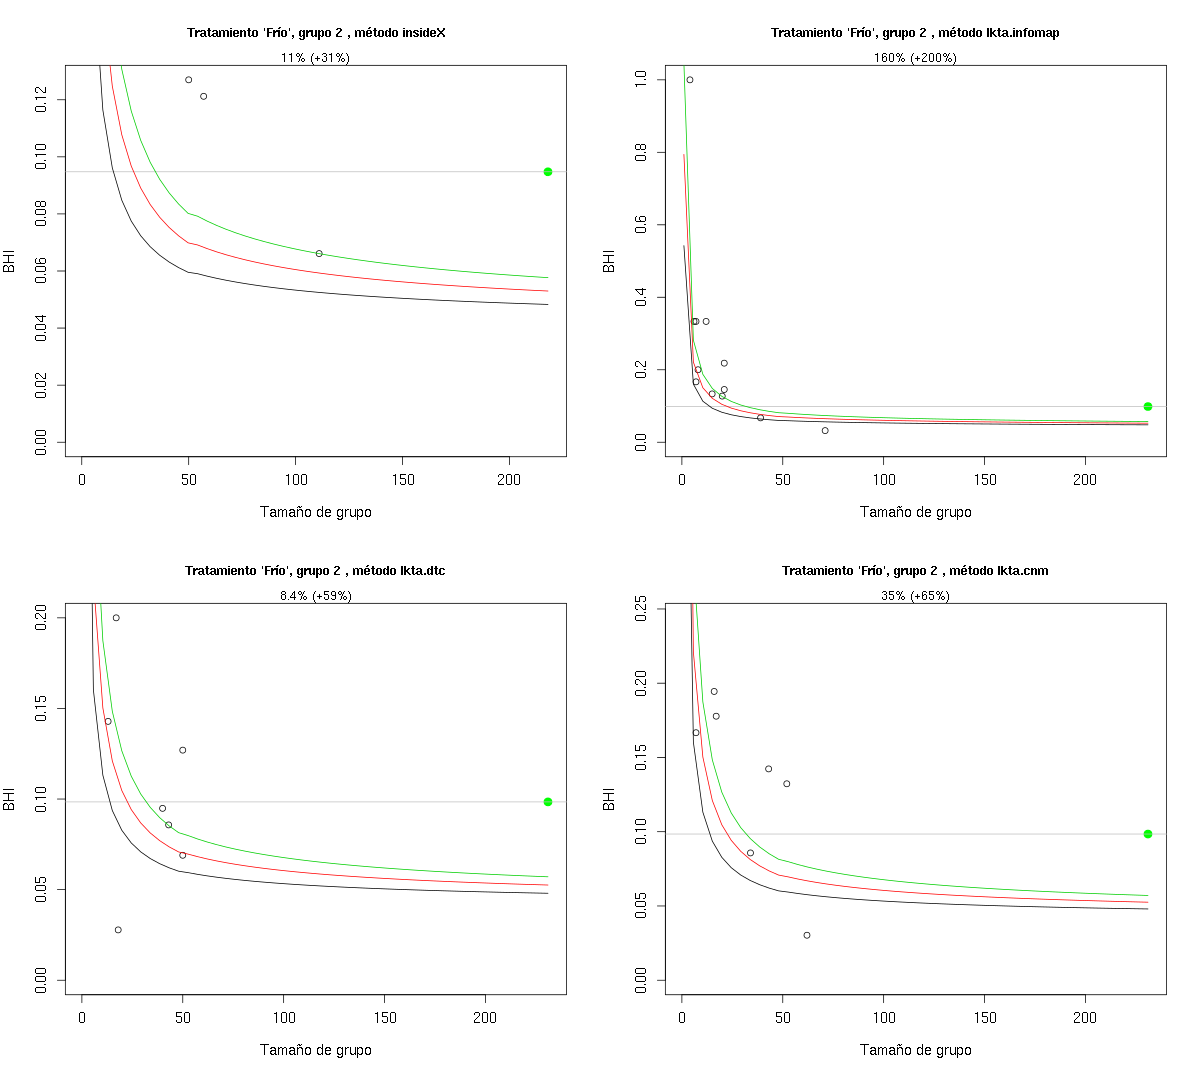
\includegraphics[width=0.7\textwidth]{metodos_mixtos_grupo_2}
\captionof{figure}{Métodos con métrica mixta y control para el grupo 2 del tratamiento 'Frío'. La curva negra indica 1 $\sigma$, la roja 2 $\sigma$ y la verde 3 $\sigma$ de la distribución del BHI del control nulo 1. El punto lleno representa el grupo original y su BHI. En verde si su BHI supera el control nulo y en rojo si no. Los puntos vacíos en gris representan los subgrupos nuevos. En la leyenda, el primer número es $\langle BHI \rangle$ y el segundo, entre paréntesis, es $\langle BHI \rangle _{+}$.}
\label{fig:metodos_mixtos_grupo_2}
\end{sidewaysfigure}

\begin{sidewaysfigure}[H]
 \centering
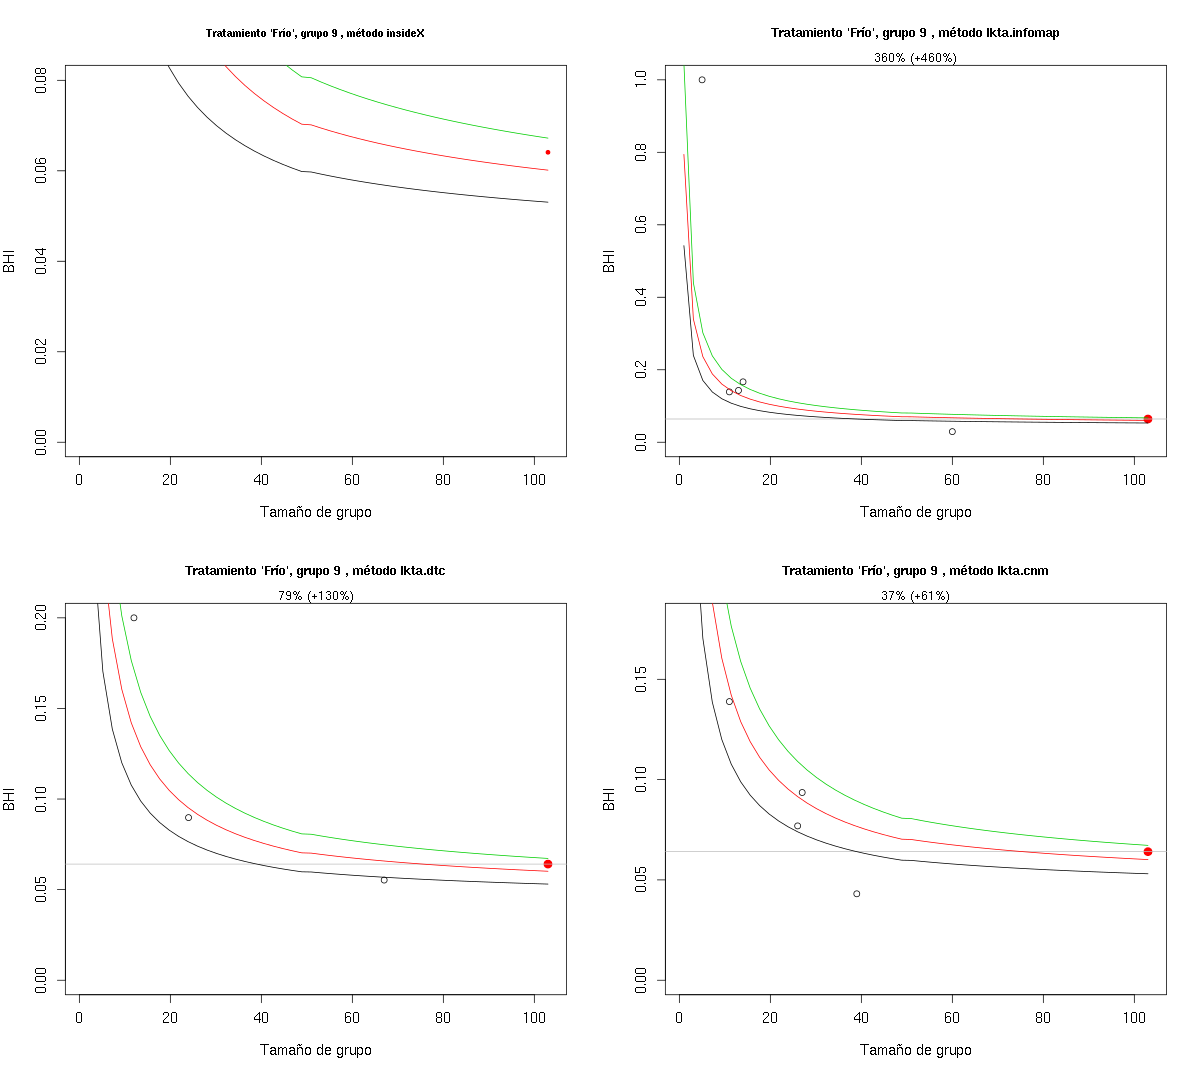
\includegraphics[width=0.7\textwidth]{metodos_mixtos_grupo_9}
\captionof{figure}{Métodos con métrica mixta y control para el grupo 9 del tratamiento 'Frío'. La curva negra indica 1 $\sigma$, la roja 2 $\sigma$ y la verde 3 $\sigma$ de la distribución del BHI del control nulo 1. El punto lleno representa el grupo original y su BHI. En verde si su BHI supera el control nulo y en rojo si no. Los puntos vacíos en gris representan los subgrupos nuevos. En la leyenda, el primer número es $\langle BHI \rangle$ y el segundo, entre paréntesis, es $\langle BHI \rangle _{+}$.}
\label{fig:metodos_mixtos_grupo_9}
\end{sidewaysfigure}

\clearpage
Se observa que para el grupo 2, un grupo con un BHI por sobre el control nulo y el segundo grupo más grande de la partición, el método \textit{insideX} logró encontrar heterogeneidades y partir el grupo, obteniendo tres subgrupos de más de 50 genes cada uno y una mejora del 11\% en $\langle BHI \rangle$, y una del 31\% para $\langle BHI \rangle _{+}$. Por otro lado, los tres métodos \textit{lkta} lograron superar la mejora obtenida por \textit{insideX} en $\langle BHI \rangle _{+}$, y tanto \textit{lkta.infomap} como \textit{lkta.cnm} lograron mejorar además el obtenido en $\langle BHI \rangle$, siendo \textit{lkta.infomap} el que mejores puntajes logró, llegando a obtener incluso un grupo con un BHI de $0.97$.\\\\
Para el grupo 9, un grupo con un BHI por debajo del control nulo y relativamente pequeño, el método \textit{insideX} no logró encontrar heterogeneidades dentro del grupo y por lo tanto no pudo particionarlo, sin lograr ningún tipo de mejora en el mismo. Sin embargo, todos los métodos \textit{lkta} lograron particionar el grupo y mejorar ambos índices, siendo nuevamente \textit{lkta.infomap} el que logró la mejora más significativa, con un 360\% de incremento en $\langle BHI \rangle$ y un 460\% de incremento en $\langle BHI \rangle _{+}$.\\\\
Finalmente, realizamos este análisis para todos los tratamientos y todos los grupos en cada tratamiento. Para cada método, graficamos el $\langle BHI \rangle$ de los subgrupos en función del BHI del grupo original en la figura \ref{fig:bhi_nuevo_vs_bhi_original}. En rojo, graficamos una recta de pendiente unitaria. Se observa que todos los métodos que utilizan la métrica mixta consiguieron grupos que no solo presentan altos valores de coherencia transcripcional sino que tienen BHI superiores a los que tenían originalmente. En particular, para lkta.infomap el 92\% de los grupos fue dividido en subgrupos que poseen un BHI promedio superior al de su grupo original, mientras que lo mismo sucede en un 91\% de los grupos para lkta.cnm y un 87\% para lkta.dtc. Finalmente, para el control insideX, solo el 10\% de los grupos mejoró su BHI promedio al ser particionado nuevamente.
\begin{center}
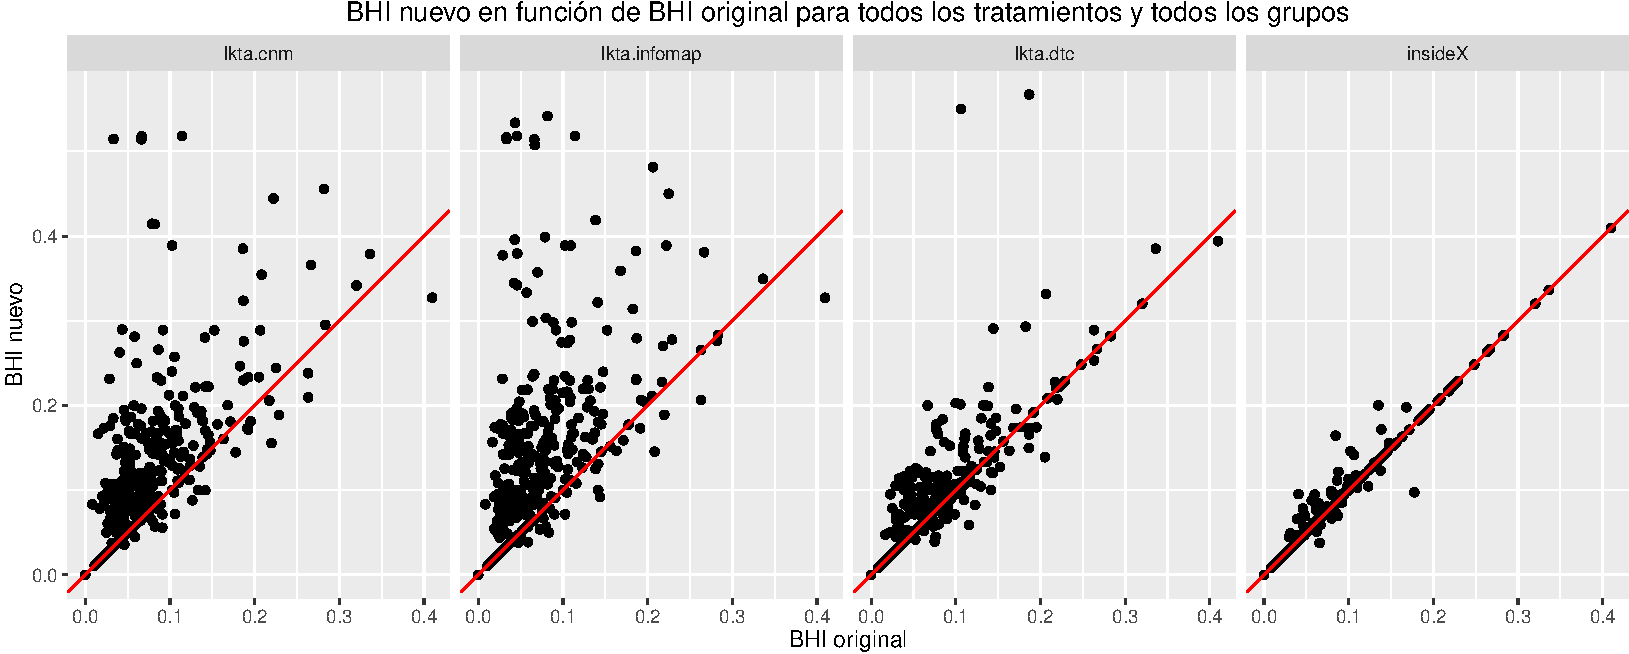
\includegraphics[width=0.8\textwidth]{bhi_nuevo_vs_bhi_original_p.pdf}
\captionof{figure}{BHI nuevo en función de BHI original para todos los tratamientos, todos los grupos y los cuatro métodos heurísticos. En rojo, una recta de pendiente unitaria.}
\label{fig:bhi_nuevo_vs_bhi_original}
\end{center}
\section{Interpretación biológica}
Una vez obtenidos los nuevos grupos mediante los distintos métodos, buscaremos ganar conocimiento sobre el significado biológico de cada grupo y en particular estudiaremos si los genes dentro de un mismo grupo participan de algún proceso biológico común. Para ello, recurriremos al análisis de sobreexpresión de conceptos GO dentro de un dado agrupamiento de genes.\\\\
El mismo consiste en considerar un grupo de genes y analizar si existen categorías de una ontología (BP u CC), sobrerepresentadas en el mismo, utilizando una prueba de Fisher exacta con un p-valor $<10e-4$.\\\\
Ilustraremos los resultados de esta tipo de análisis considerando los grupos 2, 6 y 13 del tratamiento 'Frío'. En la figura \ref{fig:metodos_mixtos_2_6_13} se observan los grupos originales y los subgrupos obtenidos por medio de cada método junto con el control nulo 1 y los correspondientes valores de BHI, mientras que en las figuras \ref{fig:fisher_grupo_2}, \ref{fig:fisher_grupo_6} y \ref{fig:fisher_grupo_13} se visualizan los resultados de la prueba exacta de Fisher para cada uno de estos grupos.
\clearpage
\begin{center}
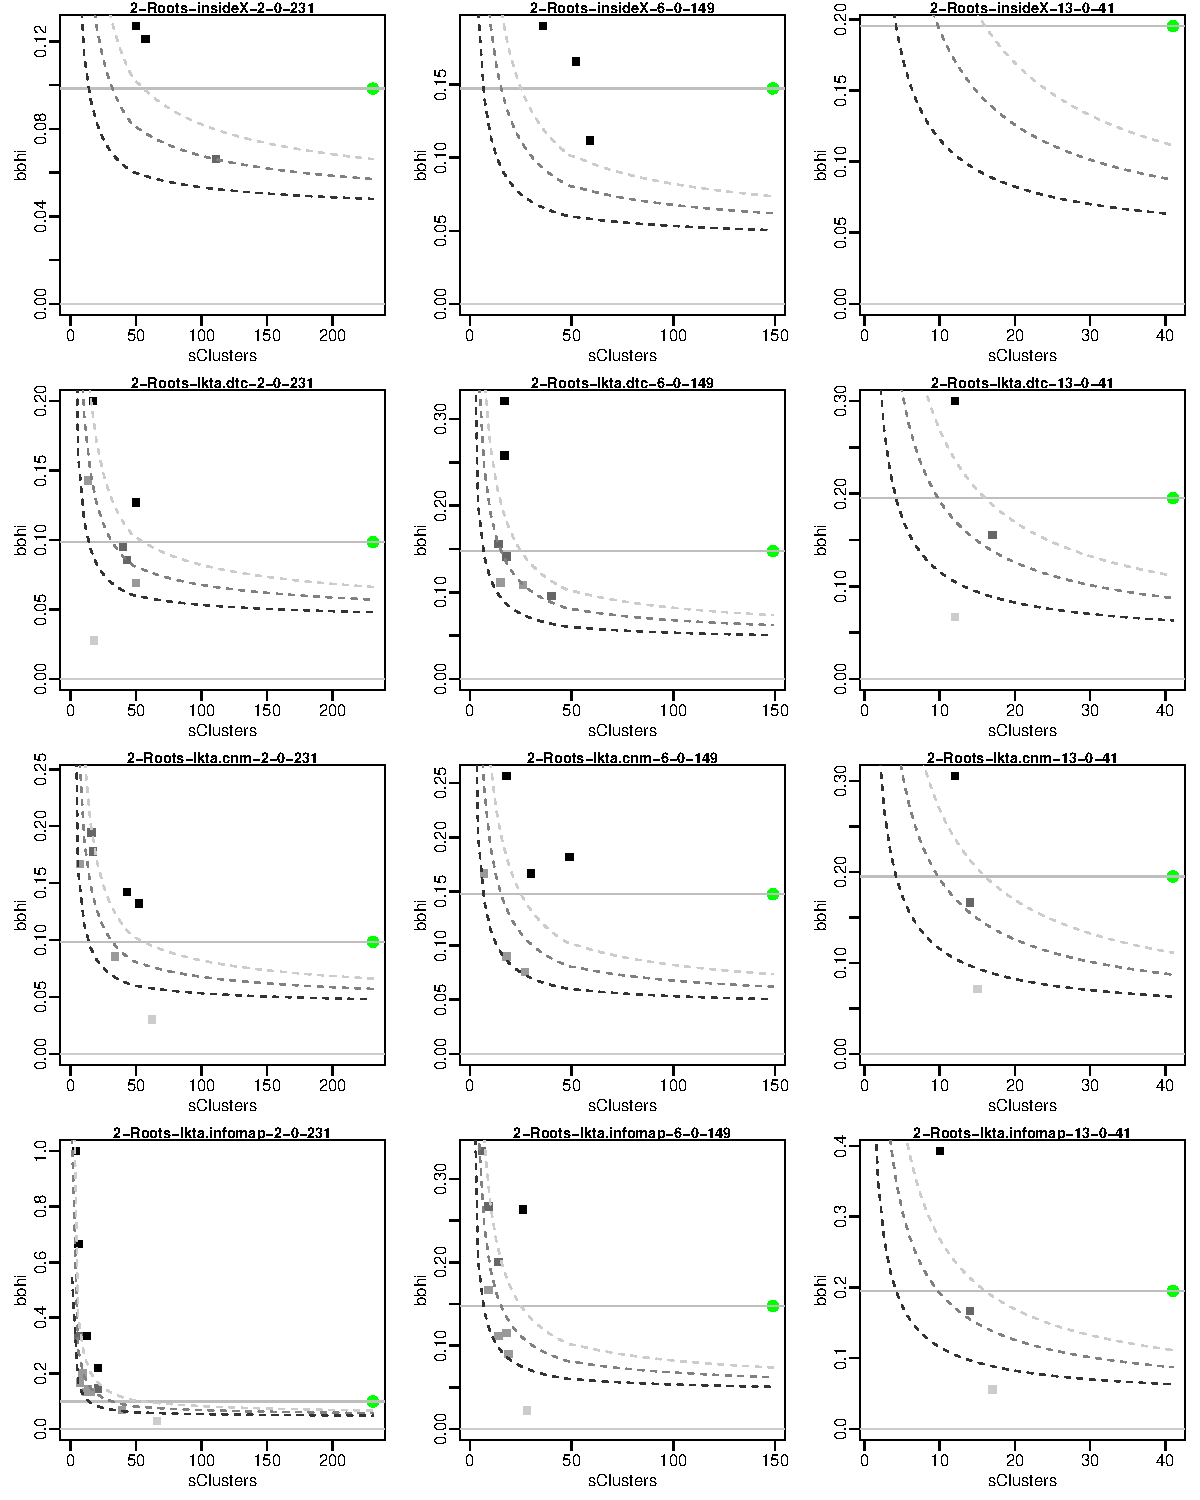
\includegraphics[width=0.8\textwidth]{metodos_mixtos_2_6_13}
\captionof{figure}{En la primera, segunda y tercera columna se consignan los resultados del análisis para grupos transcripcionales 2, 6 y 13 del tratamiento 'Frío' respectivamente. La primer, 2da y 3era fila muestran los métodos dtc, cnm e infomap. El círculo verde representa el grupo original. Los cuadrados son subgrupos, con el nivel de grisado dependiente del alejamiento de las curvas de control. Las curvas punteadas son 1 $\sigma$, 2 $\sigma$ y 3 $\sigma$ de la distribución del BHI del control nulo 1.}
\label{fig:metodos_mixtos_2_6_13}
\end{center}
En el Panel izquierdo: mapa de colores o \textit{heatmap} de p-valores donde las filas representan categorías de la ontología GOBP, y las columnas subgrupos del grupo transcripcional 2 detectados por la metodología insideX y las 3 variantes lkta.\\\\
El color corresponde al nivel de significancia obtenido en el test de sobrerepresentacion.\\\\ 
Para una mejor interpretabilidad se utilizaron los 50 conceptos GO relevantes (sobrerepresentados) mas específicos y se ordenaron según un dendrograma generado a partir de la similaridad semántica de los mismos.\\\\
Se incluye en el panel central detalle sobre el contenido de información, el nivel de profundidad en la jerarquía de la ontología y la descripción de los conceptos GO respectivos.\\\\
En el panel derecho: conceptos GO de menor especificidad para mejorar la interpretabilidad.

\begin{sidewaysfigure}[H]
 \centering
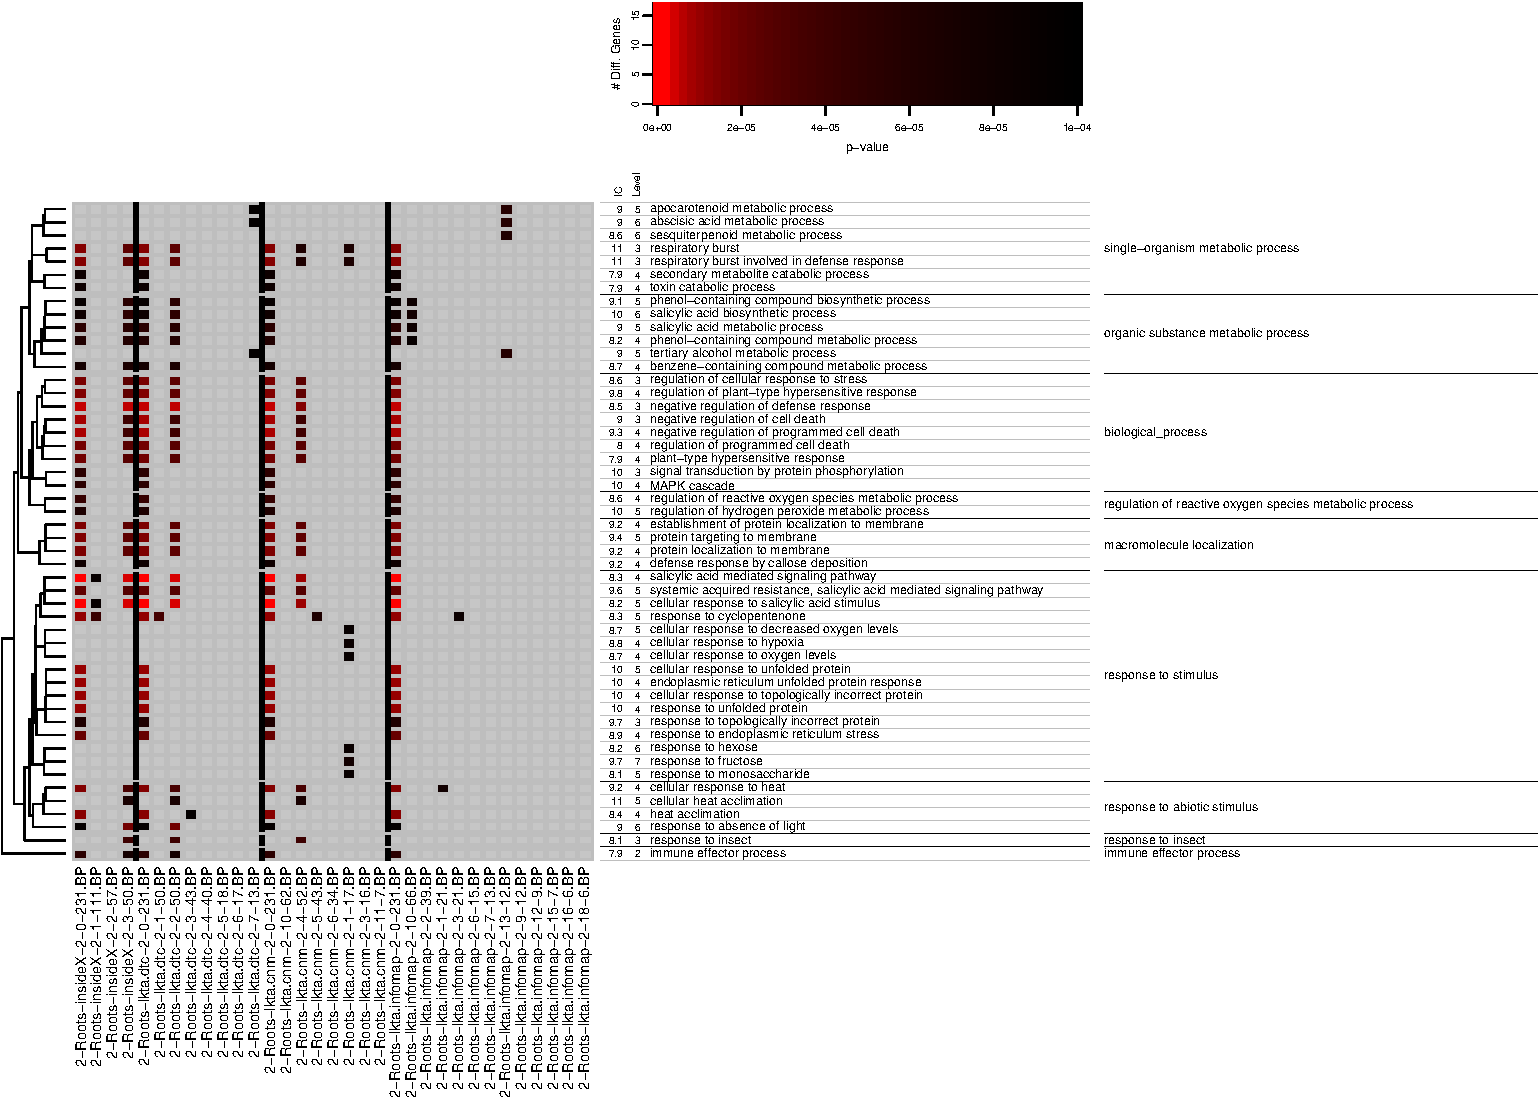
\includegraphics[width=0.9\textwidth]{fisher_grupo_2_p}
\captionof{figure}{Resultado del test de sobreexpresión de nodos GO para el grupo 2 del tratamiento 'Frío' para los métodos con métrica mixta y control.}
\label{fig:fisher_grupo_2}
\end{sidewaysfigure}

\begin{sidewaysfigure}[H]
 \centering
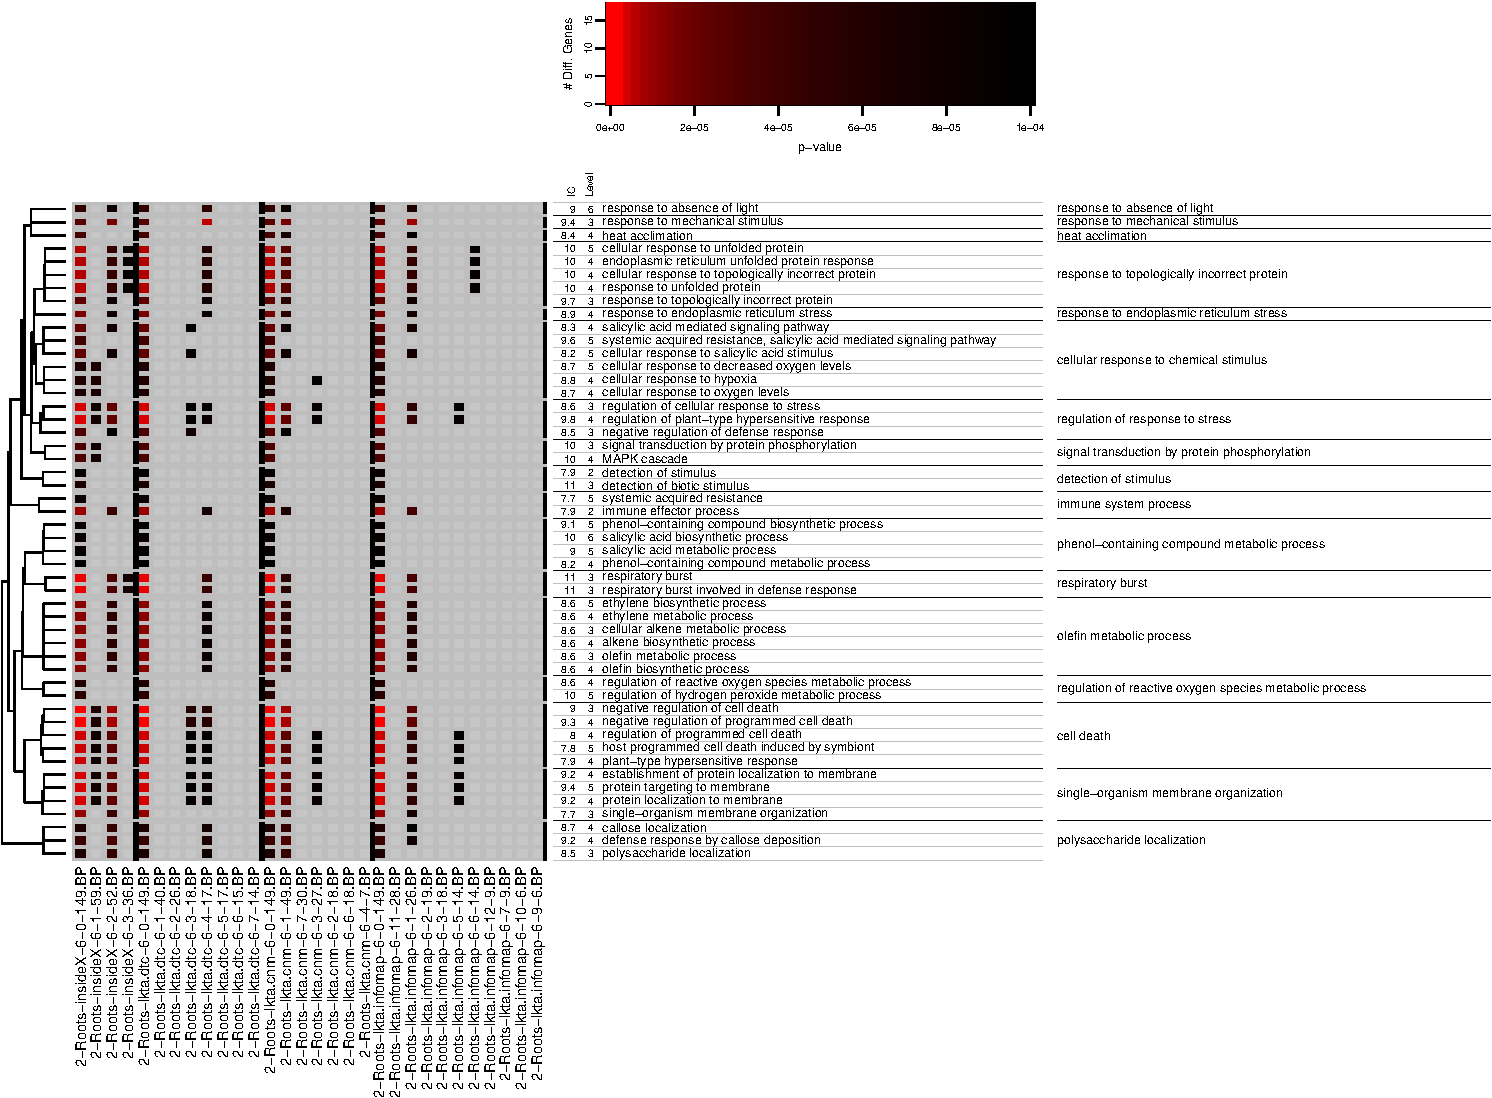
\includegraphics[width=0.9\textwidth]{fisher_grupo_6_p}
\captionof{figure}{Resultado del test de sobreexpresión de nodos GO para el grupo 6 del tratamiento 'Frío' para los métodos con métrica mixta y control.}
\label{fig:fisher_grupo_6}
\end{sidewaysfigure}

\begin{sidewaysfigure}[H]
 \centering
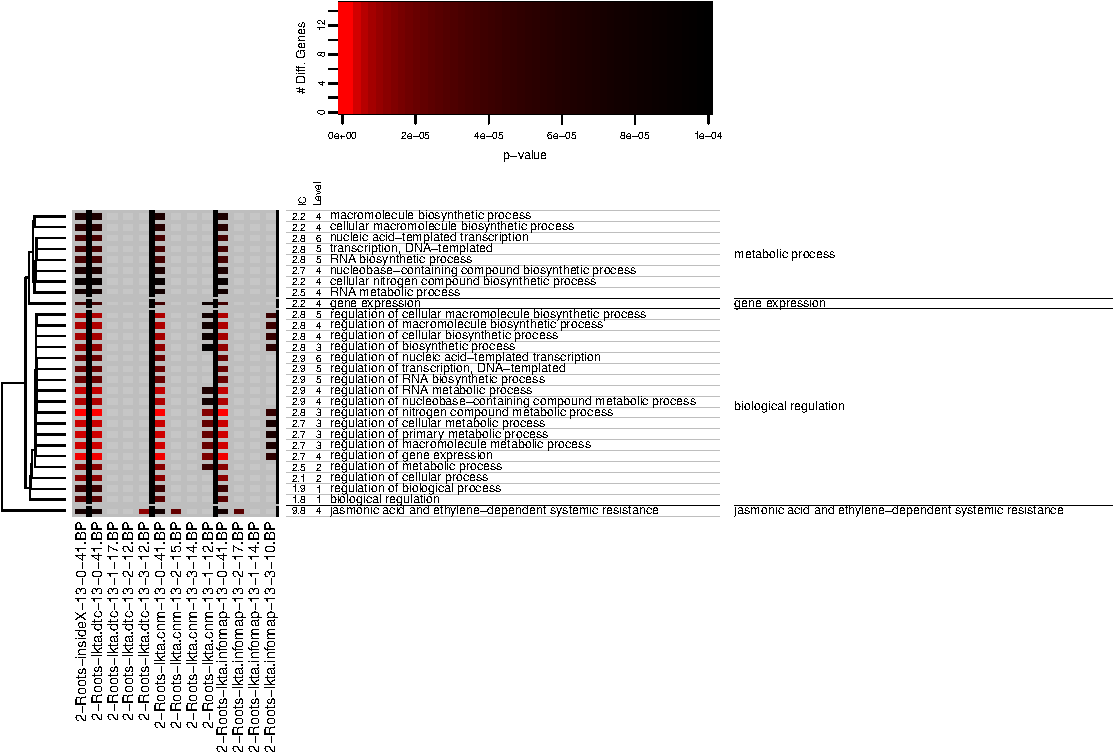
\includegraphics[width=0.9\textwidth]{fisher_grupo_13_p}
\captionof{figure}{Resultado del test de sobreexpresión de nodos GO para el grupo 13 del tratamiento 'Frío' para los métodos con métrica mixta y control.}
\label{fig:fisher_grupo_13}
\end{sidewaysfigure}

Para el grupo 2, el segundo grupo más grande de la partición, de 231 genes, y el método insideX, se observa que uno de los dos subgrupos con ganancia en BHI, el de 50 genes, explica casi en su totalidad los procesos biológicos del grupo original, mientras que no se encontró en el otro subgrupo con ganancia nodos sobreexpresados. Por otro lado, para lkta.dtc y lkta.cnmse se obtuvo un subgrupo de 50 genes con ganancia en BHI que explica los procesos del grupo original mientras que el resto de los subgrupos con ganancia no realiza aportes significativos al conocimiento biológico. Finalmente, para lkta.infomap, el de mayor ganancia en el índice BHI, ninguno de los subgrupos logra explicar los nodos sobreexpresados.\\\\
Pareciera que dentro del grupo transcripcional original (231 genes) un subgrupo de 50, detectado por 2 de las variantes lkta y la puramente transcripcional (insideX), es el responsable del enriquecimiento. El hecho de que insideX lo haya detectado sugiere que aun heterogeneidades puramente transcripcionales, puestas de manifiesto en la escala del grupo 2, correlacionan con la congruencia biológica del subgrupo.\\\\
Es interesante notar que en este caso la alta granularidad de la partición infomap parece excesiva en términos de intepretación biológica.\\\\
Para el grupo 6, un grupo de tamaño intermedio, con 149 genes, el método insideX consigue nuevamente dos subgrupos con ganancia en BHI, de 59 y 52 genes respectivamente, que explican en conjunto la mayor parte de los nodos sobreexpresados del grupo original. Para lkta.dtc se obtienen dos subgrupos informativos de tamaño pequeño, de 18 y 17 genes respectivamente. Para lkta.cnm y lkta.infomap se obtuvieron un subgrupo informativo de 49 y otro de 26 genes respectivamente.\\\\
En este caso los 3 métodos lkta detectan estructuras que se pueden asociar a los mismos conceptos biológicos.\\\\
La resolución de la partición insideX parece detectar estructuras mas grandes, pero aun permite identificar conceptos biológicos similares en relación a los subgrupos encontrados.\\\\
Finalmente, para el grupo 13, un grupo pequeño de 41 genes, el método insideX no logró producir subgrupos, mientras que solo para lkta.cnm y lkta.infomap se consiguieron grupos explicativos para un grupo de 12 y otro de 10 genes respectivamente.\\\\
En este caso, solo el uso de la metodología lkta pudo detectar subestructura relevante. Cabe notar que se trata de conjuntos muy chicos de genes, por lo que es de esperar una mayor divergencia entre la estimación de congruencia biológica dada a partir de significancia de test de sobrerepresentacion y la asociada al índice BHI (que solo exige coincidencia en un grupo, sin importar su especificidad).\\\\
En lineas generales, observamos que en varios casos una gran parte de los nodos sobreexpresados del grupo original podían ser explicados por uno o dos subgrupos de tamaño reducido, lo que implica que existen efectivamente heterogeneidades en los grupos originales que no podía detectar el método de agrupamiento inicial $ds1$. Por otro lado, las estructuras detectadas fueron de tamaños intermedios, de alrededor de 50 o 60 genes. Esto da un indicio de que esta podría ser la resolución o escala a la cual deberíamos trabajar con los métodos de agrupamiento. Finalmente, este análisis nos permite ver que si bien lkta.infomap genera las particiones de grupos con mayor ganancia en el índice BHI, los subgrupos obtenidos no necesariamente brindan información biológica. Esto podría deberse al tamaño tan reducido de los subgrupos, que no facilita su interpretación en términos de GO.





\chapter{Conclusiones y perspectivas}
La tecnología de micromatrices de ADN se constituyó como una herramienta indispensable para el monitoreo de niveles de expresión a lo largo de todo el genoma de un organismo. Las misma permiten estudiar los perfiles de expresión transcripcionales de miles de genes simultáneamente, estimando la concentración de ARNm que está siendo exportado desde el núcleo celular hacia el citoplasma para la síntesis de determinadas proteínas.\\
Mediante técnicas de agrupamiento no supervisado de datos es posible encontrar grupos de genes con perfiles de expresión correlacionados, y en particular, utilizando la distancia de correlación lineal considerada en \ref{}, es posible buscar estructuras linealmente correlacionadas. La importancia desde el punto de vista biológico de este tipo de análisis radica en que grupos de genes correlacionados   son un primer indicador de que dichos genes forman parte de un mismo proceso biológico.


Las t´
ecnicas de agrupamiento no supervisado aplicadas sobre este tipo de datos per-
miten encontrar grupos de genes cuyos perfiles de expresi´
on est´
en correlacionados. En particular,
la distancia de correlaci´
on lineal considerada (ec.2.1), compara las variaciones de expresi´
on relati-
vas a la media de cada gen, favoreciendo la b´
usqueda de estructuras correlacionadas linealmente.
Este tipo de an´
alisis es muy relevante desde el punto de vista biol´
ogico porque la detecci´
on de
grupos de genes correlacionados es el primer paso para inferir que dichos grupos participen en procesos biol´
ogicos similares.
La


%---------------HASTA ACA LOS COMENTARIOS---------------
\clearpage
\bibliographystyle{formato_bibliografia}
\bibliography{bibliografia}
\end{document}

